% Editorial policy: Use American English throughout this manuscript and in all future edits.
%%%% IJUC %%%%
\documentclass{ijuc}
% Adjust the geometry for a more common and comfortable text width
\usepackage[a4paper, margin=2.5cm]{geometry}
\usepackage[pdftex]{graphics}
\usepackage{amsmath}
\usepackage[backend=biber,style=numeric-comp,citestyle=numeric,sorting=none]{biblatex}
\usepackage{graphicx}
\usepackage{physics}
\usepackage{tikz}
\usetikzlibrary{shapes.geometric, arrows.meta, positioning}
\usepackage{epigraph}
\usepackage{amssymb}
\usepackage{algorithm}
\usepackage{algpseudocode}
\usepackage[table]{xcolor}
\usepackage{booktabs}
% ---- Color-combination table (newtab.tex) ----
\newcommand{\celliii}[9]{%
\begin{tabular}{@{}c@{}c@{}c@{}}
\scriptsize #1 & \scriptsize #2 & \scriptsize #3 \\[-2.5pt]
\scriptsize #4 & \scriptsize #5 & \scriptsize #6 \\[-2.5pt]
\scriptsize #7 & \scriptsize #8 & \scriptsize #9
\end{tabular}%
}
\newcommand{\C}[1]{\celliii{}{}{}{}{$#1$}{}{}{}{}}
\newcommand{\Cb}[1]{\cellcolor{cyan!40}\C{#1}}
\newcommand{\Cy}[1]{\cellcolor{yellow!50}\C{#1}}
\newcommand{\Csec}[2]{\celliii{}{}{$#1$}{}{}{}{$#2$}{}{}}
\newcommand{\hdr}[2]{%
\begin{tabular}{@{}c@{}}\textbf{#1}\\[-4pt]{\scriptsize #2}\end{tabular}%
}
%%%%%%%%%%%%%%%%%
\newtheorem{definition}{Definition}[section]
\addbibresource{manuscript.bib}
% Adjust tables row height
\renewcommand{\arraystretch}{1.5}
% Make COMMENT truly inline, no line break
\newcommand{\InlineComment}[1]{\quad\texttt{// #1}}
\emergencystretch=3em
\begin{document}
\title{It from bit: a concrete attempt}
\author{Alexandre Furtado Neto\inst{1}\email{alexandre.com@yahoo.com}
}
\institute{Independent Researcher}
\def\received{\today}
\maketitle
\begin{abstract}
\sloppy
We introduce a fully specified deterministic cellular automaton as a concrete test of Wheeler's ``it from bit'' idea. Space is a three-dimensional torus with periodic boundaries, plus a non-spatial internal dimension split into two sectors. Each cell stores a fixed-length binary word that evolves through local rules built from classical logic and elementary arithmetic. Wave propagation is limited to a finite speed by updating cells in discrete layers.
The model produces structures that resemble familiar physics. Waves obey a discrete wave equation with a tunable dispersion relation. Stable, self-reinforcing patterns behave like particles: they move, collide, exchange momentum, and can be created or destroyed in pairs, while conserving global counts. Interactions among these patterns show signs of attraction, repulsion, and orbit-like bound states. Probabilistic-looking behavior arises from deterministic rules because the finite state space can be coarse-grained in many equivalent ways. A built-in temporal direction comes from irreversible update steps and memory buffers. Charge-like quantum numbers appear as conservation laws tied to internal-sector symmetries; particle-antiparticle pairing arises from complementation rather than from any built-in asymmetry.
We carefully label each claim as a postulate defining the model, a measured result of simulations, or a conjecture still to be proved.  The quantitative core is a pre-registered falsification campaign: six candidate derivations of the fine-structure constant, fixed before the runs, all fail at accessible lattice sizes, and the superposed-seed aggregation hypothesis is refuted. We do not claim to recover known physics; we report a complete discrete toy universe, the tests it passes and fails, and the ideas proposed to close the remaining gaps.
\medskip{}
\end{abstract}
\vfill
\begin{center}
\textbf{PACS numbers: }12.10.Kt, 03.65.Ta, 04.60.Pp, 05.45.-a
\par\end{center}
\begin{center}
\textbf{Keywords}: cellular automaton, digital physics, maximum information speed, charge quantization, non-signaling, spherical wavefronts
\par\end{center}
\newpage
%%%%%%%% INTRODUCTION %%%%%%%%%%
\epigraph{``It always bothers me that, according to the laws as we understand them today, it takes a computing machine an infinite number of logical operations to figure out what goes on in no matter how tiny a region of space, and no matter how tiny a region of time. Why should it take an infinite amount of logic to figure out what one tiny piece of space-time is going to do? So I have often made the hypothesis that ultimately physics will not require a mathematical statement, that in the end the machinery will be revealed, and the laws will turn out to be simple, like the checkerboard with all its apparent complexities.''}{\textit{Richard Feynman}}
\section{Introduction}
John Archibald Wheeler's 'it from bit' thesis proposes that the physical world may emerge from discrete information, with bits as the bedrock of reality~\cite{wheeler}. Cellular automata (CA) --- discrete models of space, time, and local rules --- provide a natural setting for exploring this idea, since simple rules can produce complex, physics-like behavior~\cite{wolfram,zuse,fredkin}.

This work presents a deterministic cellular-automaton universe built from classical logic, elementary arithmetic, and a minimal 3-torus topology augmented by a non-spatial internal dimension. Each cell carries a fixed-size binary string whose ontological state evolves by local rules, producing spherical wavefronts, harmonic modes, and symmetry-breaking patterns. Wave propagation is confined to a spherical cavity inside the torus, suppressing corner artifacts while preserving periodic boundary conditions. We examine how these emergent structures reproduce features reminiscent of particles, interactions, and spacetime organization. The model is not offered as an interpretation of quantum mechanics, but as a primitive descriptive layer.

\emph{Claims and status.} To keep claims commensurate with evidence, every substantive statement below is graded as one of: (P) a postulate that defines the rule; (M) a measured result of the reference implementation on a small lattice; or (C) a candidate mechanism or conjecture that the current implementation does not yet establish.  The model-definition sections contain the postulates and the measurements; the particle taxonomy, the quantum-formalism mapping, and the prospects are explicitly labeled conjectural.  The paper does not claim that this automaton reproduces physics: it reports a fully specified discrete toy universe, the quantitative tests it fails or passes, and the candidate mechanisms proposed to close the gaps.  Chief among those tests is a pre-registered falsification campaign: six candidate derivations of the fine-structure constant, fixed before the runs, all fail at accessible lattice sizes (Sect.~\ref{subsec:scaling}), and the superposed-seed aggregation hypothesis is refuted (Sect.~\ref{subsec:island-candidates}); the negatives are reported as results, not hidden.

One interpretive choice governs the entire construction and should be stated from the outset. The constant velocity at which spherical wavefronts expand --- one lattice cell per tick --- is \emph{not} the speed of light. It is the maximum speed of information transmission, $v_{\max}$, a fundamental constant of the fabric. The speed of light $c$ is emergent: it is the value that an observer (Sect.~\ref{subsec:observers}) assigns to $v_{\max}$ under the round-trip measurement convention of Sect.~\ref{subsec:special-relativity}. Thus $c$ is a property of the measuring structure, not of the transition rule. Conversely, some operations of the model --- encounter and the other globally coordinated updates --- are superluminal in coordinate terms, yet they carry no capacity to transmit information and cannot be manipulated by any observer. In the idealised local rule, causality is thereby protected by construction: every influence that can be emitted, read, or steered propagates at or below $v_{\max}$.  For the host-side scheduler of the present implementation this remains to be established; the caveat is restated where non-local coordination is introduced (Sect.~\ref{sec:light-frame}) and in the formal discussion of Sect.~\ref{subsec:nosignaling-formal}.

Our construction extends foundational work in digital physics: Zuse's discrete universe~\cite{zuse}, Fredkin's reversible computation~\cite{fredkin}, and Wolfram's complex behavior from simple rules~\cite{wolfram}. The proposal is a layered 3-torus with explicit interaction rules; whether those rules reproduce quantum-like or relativistic effects is the question this paper tests, not an assumption.

The paper is organized as follows. Section~\ref{sec:related-work} reviews previous work. Section~\ref{sec:space-and-time} defines the universal fabric, and Section~\ref{initial-state} builds the initial state. The phase step and the emergent wave fields are described in Section~\ref{sec:phase-step}; the light frame in Section~\ref{sec:light-frame}. Section~\ref{sec:Interactions} details bubble interactions; the composite-particle taxonomy is deferred to Appendix~\ref{sec:Particles}. Section~\ref{sec:dynamic-charge-quantization} addresses the dynamic organization of $W$-islands, and Section~\ref{sec:Results} reports the key results; the charge-combination census is deferred to Appendix~\ref{sec:charge-census-appendix}. The speculative bridge to the quantum-mechanics formalism is likewise confined to Appendix~\ref{sec:bridge}. Section~\ref{sec:Prospects-and-conjectures} collects the remaining conjectures (the only conjectural chapter apart from the appendices), and Section~\ref{sec:Discussion} closes with a synthetic interpretation.

\subsection*{Glossary of proprietary terms}
For readability, the following model-specific terms are collected here with one-line definitions; the section in brackets is where each is first defined or used.
\begin{center}
\begin{tabular}{|l|p{0.62\linewidth}|c|}
\hline
\textbf{Term} & \textbf{Meaning} & \textbf{Sect.}\\
\hline
Orbis / Umbra & the two sectors of the internal dimension, indexed by the weak bit $w_1$ (Sect.~\ref{subsec:The-cell-structure}); each cell's charge word carries one sector bit & \ref{subsec:The-cell-structure}\\
\hline
bubble & a spherical wavefront emitted by one source center in one layer $w$; the elementary extended object of the model & \ref{subsec:pairs}\\
\hline
era & one complete wavefront expansion-and-contraction cycle; distinct from a light frame and from a housekeeping tick $k$ & \ref{sec:light-frame}\\
\hline
chief (K) & the leading source of a $W$-island; delegates (D) are attached to it, singletons (S) are free sources, and a pair (P) is a charge-complementary bonded pair of sources & \ref{subsec:pairs}\\
\hline
drive pair & an affinity-bound photon-type pair carrying $\boldsymbol{m}\ne\mathbf{0}$; its $P\times K$ and $P\times D$ contacts sustain island motion; it cannot join a cluster & \ref{subsubsec:drive pair}\\
\hline
cluster & a group of superposed equal-status pairs with the gluon/photon charge geometry $R2$ & \ref{subsec:pairs}\\
\hline
homing & the $homB$ flag stage of the light frame that drives the relocation vector $c$ toward a target & \ref{subsec:algorithm}\\
\hline
$s2B$ sieve & the electroweak gate $((u\cdot t)\bmod S)<u$ that admits a fraction of the overlapping active cells to the interaction branch & \ref{sec:phase-step}\\
\hline
Hofer effect & the conjectured radial alignment of the spins of a localized particle (Sect.~\ref{subsec:hofer}) & \ref{subsec:hofer}\\
\hline
\end{tabular}
\end{center}
\section{Related work}
\label{sec:related-work}

The hypothesis that the physical universe may be fundamentally discrete and computational has a long history in theoretical physics. Our construction builds upon several foundational programs in digital physics, extending them with a specific layered topology and interaction ruleset.

\subsection*{Early digital physics and reversible computation}
The notion of a computing universe traces back to Zuse~\cite{zuse}, who proposed in \emph{Rechnender Raum} that space and time are discrete and that physical processes arise from local, rule-based state transitions on a grid of finite-state machines. Zuse introduced ``digital particles'' as localized, self-reproducing lattice patterns and explored how continuum physics might emerge from discrete dynamics. This vision was formalized by Fredkin~\cite{fredkin} through the \emph{Finite Nature Hypothesis}, which posits that the universe is a cellular automaton (CA) whose evolution strictly preserves information. 

Because standard CA updates are often dissipative, Fredkin and Margolus~\cite{margolus} developed reversible computation frameworks. Margolus introduced block cellular automata (the Margolus neighborhood), demonstrating that permutations on shifting blocks can conserve mass, energy, and momentum directly from bit-level dynamics. These lattice-gas models proved that discrete, local, invertible rules can reproduce continuum equations at coarse-grained scales, establishing that CA-based frameworks are capable of capturing key symmetries of physical law.

\subsection*{Modern interpretations and hypergraph models}
More recently, the discrete hypothesis has been invoked to address foundational issues in quantum mechanics and spacetime. 't~Hooft~\cite{thooft} proposed a deterministic CA interpretation of quantum mechanics.  In that interpretation, quantum states are coarse-grained equivalence classes of deterministic ontological CA states, and the Hilbert-space formalism is reconstructed from classical CA dynamics via information loss at the Planck scale. 

Concurrently, Wolfram~\cite{wolfram,wolfram2020physics} has championed the computational universe hypothesis, arguing that simple CA rules (such as Rule~110) can generate the complexity required for universal computation. His recent Wolfram Physics Project generalizes CA from grid cells to hypergraph nodes updated by rewrite rules, aiming to derive spacetime and relativistic invariance from pure graph rewriting. 

\subsection*{Lattice-gas and lattice-Boltzmann automata}
A distinct tradition uses reversible block cellular automata as lattice gases that reproduce continuum hydrodynamics from purely local integer rules.  Hardy, Pomeau and Pazzis introduced the HPP lattice gas \cite{hardy1976}; Frisch, Hasslacher and Pomeau showed that a hexagonal lattice removes the spurious anisotropy of the square HPP model and yields the Navier--Stokes equation in the macroscopic limit \cite{frisch1986}.  The FHP model is the paradigmatic example of a deterministic, local, integer rule whose coarse-grained dynamics are those of a continuous field theory.  The present work shares that philosophy---a strictly local, integer-only rule with emergent continuous behavior---but differs in the target and in the ontological status of the continuum.  A lattice gas is a discretization of a pre-existing field: the hydrodynamic limit is a theorem, and the discrete objects are computational devices, not the particles themselves.  Here, by contrast, particle-like objects (pairs of bubbles riding spherical wavefronts) are meant to emerge directly from the microscopic rule, without an intermediate continuum.  The price of that ambition is that our continuum limit (Sect.~\ref{sec:Prospects-and-conjectures}) remains a labeled conjecture rather than a proven limit.  The gain claimed is precisely the ``strict deterministic ontology without coarse-graining'' of Sect.~\ref{subsec:purity}.  Nothing in the rule refers to a fluid, a field, or a metric, and the emergent $c$ is a reading of the fabric by an observer (Sect.~\ref{subsec:special-relativity}) rather than a parameter of a coarse-grained equation.

\subsection*{Positioning of the present work}
While these foundational works establish the plausibility of a computational substrate, they often leave the explicit mapping between bit-level rules and emergent particle phenomenology as an open program. Our work differs by proposing a concrete, strictly local, integer-arithmetic rule set on a 3-torus augmented by an internal dimension $W$. Unlike 't~Hooft's equivalence classes or Wolfram's hypergraphs, we maintain a strict deterministic ontology without coarse-graining, attempting to derive spherical wavefronts, polarization, and interaction gates (such as the electroweak sieve) directly from the microscopic transition rules.

\section{The universal fabric}
\label{sec:space-and-time}

Let $L$ be a large odd integer divisible by 3. The fundamental fabric of the model is a discrete lattice of cells arranged in a 3-torus ($\mathbb{T}^3$) topology. This finite, closed space is periodic: each boundary wraps around to its opposite edge, ensuring global continuity without physical boundaries.

Beyond the three spatial dimensions, the framework includes a compact internal dimension of $W$ discrete positions (referred to as \emph{layers}). Positions in $W$ do not represent additional spatial directions; rather, they serve as internal addresses that group bubbles by shared charge bits (Sect.~\ref{subsec:w-islands}). The internal organization in $W$ is essential for the continuous dissociation and reconstruction of collective structures. Stable three-dimensional particles emerge as coherent islands whose constituent bubbles remain correlated in physical space. During scattering or annihilation events, these islands may dissolve into individual bubbles, which subsequently reorganize through new pairing processes, allowing new collective structures to emerge while conserving the total bubble population.

The size of the internal dimension is defined as
\begin{equation}
W = 3L^2.
\end{equation}
Its quadratic scaling naturally matches the characteristic cross-sectional scaling of the discrete three-torus and provides sufficient internal degrees of freedom for the continual pairing, dissociation, and reorganization of bubbles. A dynamical motivation for this scaling, together with the internal population $W=3L^2$ and its $9L$ seed charge families, is given in Section~\ref{sec:dynamic-charge-quantization}.

\subsection{The cell structure}
\label{subsec:The-cell-structure}

Each cell carries the same fixed-size bit string, formatted as shown in Table~\ref{tab:Cell-structure}. Evolution progresses in uniform steps, with the input and output ports of each cell conceptually linked through a Finite State Machine (FSM). The cell state is partitioned into physical properties, wavefront shaping variables, and operational variables.

\medskip\noindent\textbf{Physical properties.} The physical role of the cell state is summarized in Table~\ref{tab:Cell-structure}.
\begin{itemize}
\item \textbf{Charge ($ch$)}: A six-bit word encoding discrete properties that govern interactions and force emergence (detailed in Sect.~\ref{subsec:charges}).
\item \textbf{pBit ($pB$)}: Marks the local in-phase sign of the emergent polarization pair $(\mathrm{pol}_u, \mathrm{pol}_v)$ reconstructed from the broadcasted arrival stamp $b(x)$. It is true when the in-phase component $\mathrm{pol}_u$ is positive ($pB = (\mathrm{pol}_u > 0)$), triggering the electric interaction channel.
\item \textbf{sBit ($sB$)}: Signals the emergent transverse polarization of the cell. It is true when the reconstructed transverse component $\mathrm{pol}_v$ is positive ($sB = (\mathrm{pol}_v > 0)$).
\item \textbf{Affinity ($a$)}: An integer variable that groups layers into particles, facilitating the aggregation of smaller units into complex entities. It is the substrate for the emergent phenomenon of entanglement and characterizes the track left by particles in self-interference.
\end{itemize}

\medskip\noindent\textbf{Wavefront shaping.}
These variables form the mechanism for nearly perfect spherical wave propagation under discrete constraints.
\begin{itemize}
\item \textbf{Dynamic squared radius ($r^2$)}: The squared Euclidean distance from the current wave source, updated locally by an incremental rule through the 6-neighborhood. It is $\mathrm{INF}$ before the wavefront reaches the cell.
\item \textbf{Dynamic radius ($r$)}: The integer radius propagated alongside $r^2$ and corrected by local square-boundary tests; it is used in the wave equation, shell forcing, and boundary absorption.
\item \textbf{Wavefront active ($\mathit{active}$)}: A boolean flag true when the cell currently lies on the pulsating spherical wavefront. It is computed by comparing the cell's propagated integer radius $r$ with the local frame radius $\mathrm{effective\_t}(t)$, which advances one cell per frame at the maximum information speed $v_{\max}$.
\item \textbf{Wave phase ($f$)}: The triangular breathing phase of the wavefront, $f = \mathrm{effective\_t}(t)$. It rises one cell per frame from $0$ to $L/2$ on the expansion branch of an era and falls back to $0$ on its contraction branch (Sect.~\ref{sec:light-frame}).
\item \textbf{Wavefront tick ($t$)}: A local physical clock providing a step counter for the maximum speed of information transmission $v_{\max}$.
\end{itemize}

\medskip\noindent\textbf{Operational variables.}
The model performs operations---translation, encounter, and wavefront propagation---that must be coordinated across the lattice. Such coordination is supported by the distinction between two clocks. The housekeeping tick $k$ is incremented synchronously in every cell and acts as an atemporal, global phase clock for the FSM. The wavefront tick $t$, on the other hand, is a local physical clock: it is reset at each source and may differ across layers and regions. The interplay between the common $k$ and the local $t$ allows the framework to schedule essentially non-local processes (encounter and coordinated updates) without endowing them with any capacity to transmit information: such processes are superluminal in coordinate speed and are intended to be strictly non-signaling, protecting causality.  For the host-side scheduler used by the current implementation, this non-signalling property is a design goal rather than an established fact (see the discussion in Sect.~\ref{subsec:nosignaling-formal}).

\begin{itemize}
\item \textbf{Translation offset ($\mathbf{c}$)}: An integer vector determining the reissue address, guiding the position where an element is reallocated within the system. The displacements follow the general rule $d_i = (t_i - c_i + L) \bmod L$, where $c_i = (L-1)/2$ for an odd $L$.
\item \textbf{Housekeeping tick ($k$)}: An atemporal clocking mechanism used for maintaining internal processes.
\item \textbf{Sieve test result ($s2B$)}: A Boolean bit seeded at each wave step from the local wave displacement $u$ and the step counter $t$. For $u > 0$ on an active cell, the deterministic test $((u \cdot t) \bmod \mathrm{SHELL\_TARGET}) < u$ produces a trigger, where $\mathrm{SHELL\_TARGET} = 16384$. The stored value is gated by the active flag, $s2B = \mathit{active} \land \mathit{trigger}$. Electroweak interaction occurs only when this bit is true.
\item \textbf{Collapse flag ($kB$)}: Indicates the occurrence of collapse in the interaction, warning the components of a particle.
\item \textbf{cluster flag ($bB$)}: Indicates whether the pair can participate in a cluster (a group of superposed pairs with the same affinity, same $bB$ bits, and the same active $pB$).
\end{itemize}

\begin{table}[htbp]
\centering
\caption{Cell state structure. Types: N (integer), DN (double integer), V (3D integer vector), B (boolean), B6 (six-bit word). The charge word $ch$ is ordered $w_1 w_0 q c_2 c_1 c_0$ (most significant bit first), matching the implementation of Ref.~\cite{af_neto}. Bit values: $q \in \{+, -\}$; $w_1 \in \{O \text{ (Orbis)}, U \text{ (Umbra)}\}$; $w_0 \in \{R \text{ (Right)}, L \text{ (Left)}\}$; $c_2 c_1 c_0 \in \{N, R, G, \bar{B}, B, \bar{G}, \bar{R}, \bar{N}\}$.}
\label{tab:Cell-structure}
\renewcommand{\arraystretch}{1.2}
\begin{tabular}{|l|c|c|l|}
\hline
\textbf{Name} & \textbf{Type} & \textbf{Symbol} & \textbf{Observations} \\
\hline
\textbf{Physical properties} & & & \\
\hline
charge & B6 & $ch$ & bits $w_1, w_0, q, c_2, c_1, c_0$ \\
pBit & B & $pB$ & local in-phase sign, $pB = (\mathrm{pol}_u > 0)$ \\
sBit & B & $sB$ & emergent transverse polarization, $sB = (\mathrm{pol}_v > 0)$ \\
affinity & N & $a$ & groups bubbles into particles \\
position & V & $\boldsymbol{x}$ & spatial coordinates \\
\hline
\textbf{Wavefront} & & & \\
\hline
dynamic squared radius & DN & $r^2$ & squared distance from the wave source \\
dynamic radius & DN & $r$ & integer Euclidean radius from the source \\
wavefront active & B & $\mathit{active}$ & true when $r = \mathrm{effective\_t}(t)$ \\
wavefront tick & DN & $t$ & clocking of the maximum information speed \\
wave phase & DN & $f$ & triangular breathing phase $f = \mathrm{effective\_t}(t)$ \\
broadcast stamp & DN & $b(x)$ & arrival tick of the elected-momentum news \\
polarization $u$ & N & $\mathrm{pol}_u$ & in-phase reconstructed polarization component \\
polarization $v$ & N & $\mathrm{pol}_v$ & transverse reconstructed polarization component \\
\hline
\textbf{Operational variables} & & & \\
\hline
translation offset & V & $\mathbf{c}$ & determines reissue address \\
momentum vector & V & $\boldsymbol{m}$ & integer momentum, typically $\lvert\boldsymbol{m}\rvert=L/2$; immutable under inertia \\
translation impulse & V & $\mathit{reloc}$ & consumable signed displacement; filled by encounter, applied by \texttt{applyMomentum} \\
housekeeping tick & DN & $k$ & timeless clocking \\
sieve test result & B & $s2B$ & seeded from $u$ and $t$, gated by $\mathit{active}$ \\
sB homing & B & $homB$ & flag to find the sB bit \\
contraction flag & B & $cB$ & marks a bubble in the contraction phase \\
collapse flag & B & $kB$ & hints collapse \\
cluster flag & B & $bB$ & marks pairs eligible for cluster formation \\
\hline
\textbf{Source model} & & & \\
\hline
source kind & N & $\mathrm{kind}$ & $K$ (chief), $S$ (singleton), $D$ (delegate), $P$ (pair) \\
pair index & DN & $\mathrm{pair\_idx}$ & partner layer of a $P$ source \\
pair count & N & $\mathrm{pair\_count}$ & superposed pairs of a $P$ source \\
\hline
\end{tabular}
\end{table}

\paragraph{The host lattices.}\label{subsec:The-host-lattice}

The spatial fabric is implemented using three coexisting 3D lattices of $L^3$ cells each, replicated across the $W$ layers (totaling $3L^3W$ cells). All cells within a layer evolve synchronously, exchanging information with their seven neighbors (six spatial, one along $W$). This exchange occurs in alternating passes, recovering time homogeneity every two clock ticks and configuring the system as a cellular automaton. The three lattices are referred to as \emph{main}, \emph{draft}, and \emph{partner}. The main lattice is the current state used in interactions; the draft lattice holds the modified data for the current tick; and the partner lattice is a snapshot used for comparisons across different $W$ addresses during the encounter stage. A cell can modify its own draft cell, but not its main cell directly.

\subsection{Purity constraints}
\label{subsec:purity}

The rules of this universe are deliberately constrained so that the model remains a \emph{pure} cellular automaton. These constraints shape the physics that the automaton can produce and are recorded here as design criteria.

\begin{description}
\item[Locality.] A cell's next state is computed only from its own current state and from the states of a fixed, finite neighborhood of adjacent cells. No cell reads global counters, hidden pointers, queues, frontier lists, or pre-computed tables that depend on the whole lattice.
\item[Synchronicity and parallelizability.] Every cell updates simultaneously from the current lattice into a second, identical lattice (\texttt{grid} and \texttt{grid\_next}). The two buffers are the only shared memory; after the tick, the roles are swapped. This makes the rule directly parallelizable.
\item[Integer-only runtime.] Inside the transition rule, all calculations use only addition, subtraction, bit shifts, and comparisons. Multiplication, division, floating-point arithmetic, square roots, trigonometric functions, and any other continuous operation of \emph{dynamic} operands are forbidden in the runtime loop. Fixed topological constants (e.g., $2R$, $L/2$, $9L$) are evaluated once at initialization and stored in read-only integer globals. Multiplication by such a constant is a fixed-strength operation, not the data-dependent multiplication the constraint excludes.
\item[No tables.] No pre-computed lookup tables encode the dynamics. Distances, phases, and interaction weights must propagate through local rules from the initial seed.
\item[Finite-state and deterministic.] Each cell contains a fixed-size bit string. The transition rule is a finite function of this string and its neighborhood, with no Turing-complete constructs, no unbounded iteration, and no randomness.
\item[Occam's razor.] The cell state is kept minimal. Auxiliary global variables, linked lists, or index arrays that point into the lattice are rejected because they would make the automaton's state depend on the order of evaluation rather than on the cell contents alone.
\item[Simple initialization.] The initial state is set by fiat only at $t=0$: a small seed is planted in an otherwise blank lattice. All subsequent structure emerges from the local rule.
\end{description}

These are target constraints, not properties already verified for the executable. In particular, the current inertial transport reference uses source snapshots, contact lists, a frame counter and periodic layer translations (Sect.~\ref{subsec:translation}); polarization preparation also uses host arithmetic. A local finite-state realization of this coordination remains open. The theoretical topology is parameterized by $L$ and $W=3L^2$, while the prepared-island experiments may allocate a reduced number of layers.

\subsection{Charges}
\label{subsec:charges}

Charges are constant-valued bits ($ch$ in Table~\ref{tab:Cell-structure}) that govern particle interactions. Inspired by the Standard Model, the six-bit charge word is partitioned into electric, weak, and color sectors. All cells in a given $W$-layer share the same charge value.

The electric charge $q$ is associated with attraction and repulsion, while the weak charge, composed of two bits $w_1$ and $w_0$ (chirality), is associated with congruence. The sector with $w_1 = 0$ is called \emph{Orbis}, while the sector with $w_1 = 1$ is called \emph{Umbra}. The three color charges $c_2, c_1, c_0$ enforce the strong force structure. Color codes are $N:000$, $R:001$, $G:010$, $\bar{B}:011$, $B:100$, $\bar{G}:101$, $\bar{R}:110$, $\bar{N}:111$ for \emph{neutral}, \emph{red}, \emph{green}, \emph{antiblue}, \emph{blue}, \emph{antigreen}, \emph{antired}, and \emph{anti-neutral}, respectively.

Let the signature be $sig = c_2 + c_1 + c_0$. A bubble is matter $M$ if $sig < 2$, or antimatter $\overline{M}$ otherwise. It is neutral $N$ if $sig = 0$, or anti-neutral $\overline{N}$ if $sig = 3$. The pBit $pB$ marks the positive in-phase half-cycle of the polarization pair, while the sBit $sB$ records the transverse sign derived from the reconstructed $(\mathrm{pol}_u, \mathrm{pol}_v)$ pair. Both emerge from the cellular dynamics rather than being precomputed path patterns.

%%%%%%%% INITIAL STATE %%%%%%%%%%
\section{Initial state}\label{initial-state}
The initial state is the only information set by fiat.  It fixes the static, non-dynamical configuration of every cell at $t=0$ and is copied to the draft lattice as well.  All dynamic quantities---the wavefront radius, the wave cloud, the polarization pair $(\mathrm{pol}_u,\mathrm{pol}_v)$, and the interactions---are generated from this seed by the same local transition rule.
\subsection{Internal addressing and $W$-islands}\label{subsec:w-islands}
The internal non-spatial dimension has size
\begin{equation}
W=3L^{2},
\end{equation}
where $L$ is a large odd integer divisible by $3$.
During the Platonic Initialization, $W$ is partitioned axiomatically into
\begin{equation}
N_{I}=9L
\end{equation}
identical \emph{$W$-islands}, each containing
\begin{equation}
\ell=\frac{W}{N_{I}}=\frac{L}{3}
\end{equation}
positions.
A $W$-island is an internal charge family: its $\ell$ copies are $\ell$ distinct $W$-addresses that share the same six charge bits but have distinct $pB$/$sB$ patterns.  Each such address maps to a distinct spatial position in the 3-torus---i.e., each copy is one bubble at one lattice site---so that the $W$-island is an abstract grouping, not a spatial substructure.
The distinct polarizations provide the internal angular diversity needed for the Hofer effect (Sect.~\ref{subsec:hofer}).
The detailed dynamics of how these copies aggregate into $1K+nD$ islands, and how the island population stabilizes, is treated in Section~\ref{sec:dynamic-charge-quantization}.
\subsection{The Platonic seed}
Among the many possible choices, we select the following deterministic Platonic seed:
\begin{itemize}
\item The spatial address $\boldsymbol{x}$ is set to the appropriate Cartesian positive coordinates ($0\ldots L-1$).  Every source center is placed at the single lattice center $\mathbf{c}=((L-1)/2,(L-1)/2,(L-1)/2)$, so that all bubbles are born superposed at one point with zero radius---deterministically and without random numbers.
\item The internal address $w$ is immutable; charge bits are derived from its charge-family index $\nu=\lfloor w/\ell\rfloor$, so copies of a family have equal charges. In the seed used for the numerical experiments, $w_0=\nu\bmod2$, $w_1=\lfloor\nu/2\rfloor\bmod2$, $q=w_1\oplus w_0$ and color $=\nu\bmod8$.
\item The affinity $a$ and the auxiliary leader identity $\mathit{leader\_w}$ are initialized to the island index of the $W$-island to which $w$ belongs (Sect.~\ref{subsec:w-islands}).  A true chief ($K$) emerges later through encounter, as described in Section~\ref{sec:dynamic-charge-quantization}.
\item The housekeeping counter $k$ and the wavefront counter $t$ are set to zero; the contraction/phase vectors $\mathbf{c}$ are zero and $s2B$ is reset.
\item The momentum vector $\boldsymbol{m}$ is initialized to $\boldsymbol{0}$. The dynamic election path may install a direction at an expansion limit, once on the frame edge. Once a pair is an affinity-bound drive pair with nonzero $\boldsymbol{m}$, its transport direction is preserved rather than replaced at every era. Prepared-island probes explicitly seed that direction to isolate the inertial mechanism.
\item The consumable translation impulse $\mathit{reloc}$ is zero.
\item The wavefront data are seeded only at the source centers: $u=v=0$ and $r^{2}=0$, with a fixed amplitude $U_{0}$; all other cells have $r^{2}=\mathrm{INF}$ and $u=v=0$.
\end{itemize}
Real numbers and high-level functions are used only as intermediaries to compute these integer parameters; they are not stored in the lattice.  The dynamics is therefore strictly integer-based.
\paragraph{What the seed does not contain.}
The seed contains no precomputed radius, no wave cloud, no $(\mathrm{pol}_u,\mathrm{pol}_v)$ pair, no $pB$/$sB$/$s2B$ pattern, no non-zero momentum $\boldsymbol{m}$, no interactions, and no randomized data.  Those are the first emergent consequences of the seed and are described in Sect.~\ref{sec:phase-step}.
\subsection{The initial thermal bath}
Dynamic initialization and evolution proceed concurrently under the same transition rules, with no global barrier between them. Their dependencies are local: one region may already sustain organized aggregates while another remains in a transient regime, and subsequent interactions may disturb previously stabilized variables.

Before the distance, polarization and island patterns settle into their operating regime, the system undergoes a preparation transient. Its proposed mixing role is a deterministic ``thermal bath''; homogeneity and loss of dependence on the seed must be measured, not inferred from irregular motion alone. Statistics intended to characterize inertia must exclude an explicitly reported preparation window and compare successive measurement windows. A discarded prefix alone is not evidence of equilibration.
%%%%%%%% PHASE STEP %%%%%%%%%%
\section{Phase step and emergent wave fields}\label{sec:phase-step}
Once the Platonic seed is fixed, the first CA ticks generate the wavefront geometry that feeds the frame FSM of Sect.~\ref{sec:light-frame}.  The subsections below describe those emergent fields.
\subsection{Dynamic radius and the Euclidean metric}\label{subsec:wavefront-metric}
The wave field is seeded at the source centers, all of which are born superposed at the lattice center.  From its source, each wavefront expands as a sphere in the cubic lattice, so we need a local, integer-valued approximation of the Euclidean distance from every cell to its source.
\paragraph{Squared-distance update.}
Let the source have integer coordinates $(c_{x},c_{y},c_{z})$ and let $(x,y,z)$ be the cell coordinates, all taken modulo $L$ along each axis of the 3-torus.  The exact squared Euclidean distance is
\[
r^{2}=(x-c_{x})^{2}+(y-c_{y})^{2}+(z-c_{z})^{2}.
\]
In the 6-neighborhood (axis-aligned moves only), an outward step along the axis with absolute offset $a$ from the source changes $r^{2}$ by
\[
\Delta r^{2}=(a+1)^{2}-a^{2}=2a+1.
\]
Therefore the local update is purely additive:
\[
r^{2}_{\text{new}}=r^{2}_{\text{old}}+2a+1,
\]
where $a$ is the cell's own absolute coordinate along the moved axis.  Each cell needs only its stored $r^{2}$ and its absolute offset from the source, both integers.  The update is performed synchronously over the whole lattice at every tick: each cell writes its new value into a second, identical lattice ($\texttt{grid}$ and $\texttt{grid\_next}$), so the rule is a local double-buffer CA transition.  In one tick a cell can only learn from its six immediate neighbors, so the reachable region grows by one lattice layer per tick, exactly as the information cone should---the cone of the maximum speed of information transmission $v_{\max}$; before the wavefront reaches a cell, $r^{2}=\mathrm{INF}$.  Because the edge weights are non-negative, repeated synchronous sweeps converge to the same minima a Dijkstra/BFS relaxation would produce, but without any global queue or frontier list.
\paragraph{Radius correction method}
Several physical formulas require the ordinary radius $r$ rather than its square:
the wave envelope $\sin(r)/r$
and the radial shell count used for the $r\cdot\sin(r)$ density use $r$ directly,
while the wave phase $f=\mathrm{effective\_t}(t)$ is the triangular breathing phase of the local tick $t$ (Sect.~\ref{sec:light-frame})---it rises one cell per frame from $0$ to $L/2$ and falls back to $0$, so over one era it selects the cloud point density over exactly the first lobe, from $0$ to $\pi$ and back.
The topological constants $2R$ and $\mathrm{phase\_full}$ remain in use for the polarization reconstruction of Sect.~\ref{subsec:polarization-pair}.
The lattice is integer-valued, so $r$ is the largest integer not exceeding the true Euclidean distance,
$r=\lfloor\sqrt{r^{2}}\rfloor$.
We propagate $r$ alongside $r^{2}$.
When a cell with radius $r$ passes the wavefront to a 6-neighbor,
the neighbor's squared distance increases by $2a+1$,
which changes the true radius by $0$ or $1$.
Hence the neighbor's integer radius is either $r$ or $r+1$,
and the correct choice is the one that satisfies
\[
(r')^{2}\le r^{2}_{\text{new}}<((r')+1)^{2}.
\]
This test uses only integer additions and comparisons.
A one-step source-center motion changes any cell's radius by at most one,
so a tiny correction loop around the previous $r$ is enough to keep the value exact after the source moves.
The discretization error is at most one lattice unit and does not accumulate,
because $r^{2}$ is re-anchored by the source center each sweep
and the radius is re-corrected from the exact $r^{2}$.
\paragraph{Efficiency of the method}
Extracting $r$ once per cell per tick would require a bounded loop of bit operations.
By propagating $r$ together with $r^{2}$ we replace that generic root extraction
by a single local square-boundary test: the parent cell already knows its own radius,
and the child radius is either the same or one larger.
The source center re-anchors $r=0$ each sweep, so errors cannot drift.
This keeps the FSM transition small and avoids carrying a full integer square-root routine in the inner loop.
\paragraph{Why the 6-neighborhood?}
The 6-neighborhood corresponds to the three Cartesian axes and is the minimal set of edges compatible with the discrete rotation/reflection symmetries of the cubic lattice.  Edge weights $(2a+1)$ then give the correct squared Euclidean increments for those edges.  Moves along face diagonals or body diagonals would require larger neighborhoods and non-integer corrections; the 6-neighborhood together with the squared-distance update already captures the Euclidean metric without adding extra edges.
\paragraph{Boundary behavior.}
Because the lattice is a 3-torus, the distance field wraps through the periodic boundaries.  The update remains local: a step that crosses a face of the cube uses the periodic coordinate and the same $2a+1$ increment.  As long as the source center is taken modulo $L$ in each axis, the resulting $r^{2}$ is the squared distance on the torus.  Multiple source centers are handled independently, one per $W$-layer, and the local relaxation within each layer does not mix their fields.
\subsection{The wave cloud}\label{subsec:Sine}
The wave cloud is not a precomputed mask. It emerges from a discrete wave field that propagates outward from each bubble. Each cell carries a wave amplitude that evolves according to an integer-only wave equation, while a pulsating spherical wavefront marks the cells whose propagated integer radius $r$ equals the local frame radius $\mathrm{effective\_t}(t)$ (which advances one cell per frame at the maximum information speed $v_{\max}$) as \emph{active}. The sieve bit $s2B$ is computed directly from the local displacement $u$: for $u>0$,
\[
\bigl((u \cdot t) \bmod \mathrm{SHELL\_TARGET}\bigr) < u,
\qquad \mathrm{SHELL\_TARGET}=16384,
\]
sets a trigger, and the result stored in the cell is $s2B = \mathit{active} \land \mathit{trigger}$. During interactions the bit is propagated as $s2B' = s2B \land \mathit{active}$. The coincidence of \emph{active} cells whose $s2B$ bit is true forms the sieve.
Because the number of cells at radius $r$ on a cubic lattice scales approximately as $r^{2}$, the radial density of active cells with $s2B$ true follows $r\cdot\sin(r)$, which is the electromagnetic coupling density (see Figure \ref{fig:wave-cloud}). The underlying wave amplitude per cell is $\sin(r)/r$, so the $r\cdot\sin(r)$ density is a geometric consequence of binning active $s2B$ cells over spherical shells. The $s2B$ bit propagates this test between bubbles.
The cloud is generated on the fly inside each light frame.  At $t=0$ the wave field is zero except for the excitations of fixed amplitude $U_{0}$ with $r^{2}=0$ at the source centers; all other cells have $r^{2}=\mathrm{INF}$ and $u=0$.  The constant $U_{0}$ is chosen independently of $L$ (for example, $U_{0}=2048$ in the reference implementation), so the same seed remains valid as the lattice grows; in the $L\to\infty$ limit it becomes a point excitation on an unbounded lattice.  As the wavefront radius expands and contracts over an era, one cell per frame (at the maximum information speed $v_{\max}$), the normalized wave amplitude yields the $\sin(r)/r$ envelope per cell, and the active-triggered cells form the $r\cdot\sin(r)$ density.  The wave phase $f$, the Bresenham accumulator, and the active flag are therefore dynamical, not imprinted by fiat.
The constants $U_{0}=2048$ and the sieve modulus $S=16384$ are \emph{free} parameters: nothing in the model fixes them; they are scale choices of the reference implementation.  Their role is now quantified: $U_{0}$ sets the amplitude scale $u$ on the active shell, and the electroweak channel opens or closes with the ratio $u/S$ (Sect.~\ref{subsec:s2b-sweep}).  The reference values were chosen so that the sieve is nearly dormant ($u/S\lesssim1\%$), i.e.\ so that the \emph{weak} channel is genuinely rare at the reference configuration; the choice $S=2^{14}$, $U_{0}=2^{11}$ also keeps the modulo arithmetic in the cheap integer range.  A principled derivation of both constants from the model is an open problem (Sect.~\ref{sec:Discussion}).
\begin{figure}
\begin{center}
\scalebox{0.8}{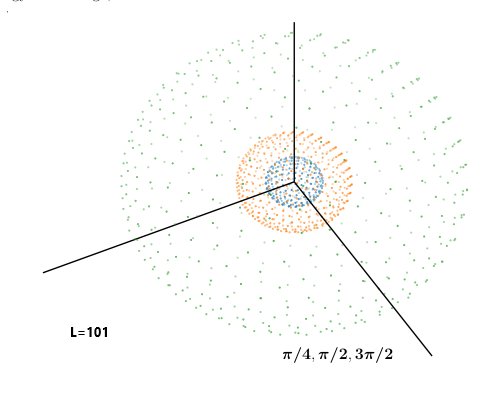
\includegraphics{fig1}}
\end{center}
\caption{The emergent $r\cdot\sin(r)$ wave cloud. \label{fig:wave-cloud} The radial interaction density of the active $s2B$ cells plotted against the radial distance $r$ from the source center (horizontal axis: integer shell radius $r=1,2,\dots$ in cells; vertical axis: normalized density of active cells on the shell).  The cell-by-cell wave amplitude follows $\sin(r)/r$, while the number of cells per spherical shell scales as $r^{2}$; their product gives the radial interaction density $r\cdot\sin(r)$ used for electromagnetic coupling.  The curve is the analytical envelope $r\sin(r)$ (arbitrary vertical scale) overlaid on the simulated shell counts; the measured match is quantified in Sect.~\ref{subsec:scaling}.}
\end{figure}


\subsection{Emergent polarization pair $(\mathrm{pol}_u,\mathrm{pol}_v)$}\label{subsec:polarization-pair}

Each active cell carries an integer pair $(u,v)$, stored as $\mathrm{pol}_u$ and $\mathrm{pol}_v$, that represents the transverse polarization in the plane tangent to the spherical wavefront.  The pair is not a geometric function of the local radius; it is derived from the \emph{broadcasted arrival stamp $b(x)$ of an elected momentum vector}.  At every turn-around of the breathing wavefront the automaton elects one direction out of its own state, a helical walker broadcasts the news of that election across the layer, and every cell converts its private arrival stamp into a polarization phase.  The mechanism has three stages---election, broadcast, and reconstruction---and uses only addition, subtraction, shift, and comparison.

\paragraph{Overview.}  The goal is to assign to each cell a direction in the plane perpendicular to an elected axis $\boldsymbol{m}$, using only integer arithmetic.  The direction is encoded as a pair $(u,v)$ lying on a circle of radius $R^2$, where $R$ is the emergent bubble radius.  The angle $\theta = \operatorname{atan2}(v,u)$ advances from $0$ to $2\pi$ as the broadcasted arrival time grows, winding a polarization helix around $\boldsymbol{m}$.  The automaton never computes $\theta$ explicitly; it computes $(u,v)$ directly from the arrival stamp using integer square roots.

\paragraph{Stage 1: Election.}  Every cell owns a predefined value $\nu\in[\,0,\,9L-1\,]$---its $W$-island index, fixed once by the internal address.  At the expansion limit of the pulse (the exact tick where the wave turns from ascending to descending), every active shell cell is seeded with a \emph{payload} that combines a score (derived from $\nu$ and a global seed $s$) with the cell's linear index.  Because the index occupies the low bits, the payload order is a strict total order: ties are impossible, so the winner is unique and independent of any scan order.

Each pass lets every cell adopt the greatest payload among its six face neighbors:
\[
\mathrm{payload}(x)\;\leftarrow\;\max\bigl(\mathrm{payload}(x),\;\mathrm{payload}(x\pm e_i)\bigr),
\]
with alternating sweep directions; $2R+8$ passes guarantee full coverage of the lattice.  The true winner---the \emph{seeded} cell holding the greatest payload---is identified once, at sowing time, while the payloads are still unique; the diffusion flood merely transports the news and never redefines the winner.  The displacement from the lattice center to the winning cell becomes the momentum vector $\boldsymbol{m}$: it is rescaled to $\lvert\boldsymbol{m}\rvert=L/2$ and written onto the source-center cell of the layer.  That write is the sole dynamic initialization of $\boldsymbol{m}$; thereafter the inertia path (Sect.~\ref{subsubsec:drive pair}) treats $\boldsymbol{m}$ as immutable and only reads it to accumulate $\mathit{reloc}$ impulses.  The same elected axis drives the helical walker of Stage~2.  The next expansion limit may elect a fresh direction; nothing is prescribed at the Platonic seed, and the orientation is read off the automaton's own ledger at the instant the wave reaches its limit.

\paragraph{Stage 2: Broadcast.}  As soon as $\boldsymbol{m}$ exists, a helical walker traces the spiral arm on the pulsating bubble.  It advances one cell per tick around the cylinder whose axis is the elected direction, keeping the radial error within about one cell by purely local comparisons among its six neighbors.  The walker is an arbitrary-axis integer helix (implementation details in the source code: \texttt{spiral/spiral.c}).  During the walk, each newly computed spiral point writes one plus the current tick into its own cell of a second value lattice, reserving $b(x)=0$ for ``never reached''.

Every other tick, with alternating sweep directions, every cell inspects only its six face neighbors and copies the greatest neighbor value whenever it exceeds its own:
\[
b(x)\;\leftarrow\;\max\bigl(b(x),\;b(x\pm e_i)\bigr).
\]
No cell ever senses beyond its neighborhood, yet these monotonic values diffuse as waves that in finite time reach every cell of the lattice---global coverage achieved purely by local moves, in lockstep with the automaton tick.  Each cell therefore ends up holding the tick $b(x)$ at which the news of the elected momentum arrived.

\paragraph{Stage 3: Reconstruction.}  The arrival stamp $b(x)$ is the phase source.  A full $2\pi$ turn is encoded by $\mathrm{phase\_full}=2R^{2}$ units, where $R=L/2-2$ is the emergent bubble radius ($R$ and $\mathrm{phase\_full}$ are topological constants, Sect.~\ref{subsec:purity}).  The cell phase is read directly from the broadcasted value:
\[
\mathrm{cell\_phase}=(b(x)-1)\bmod\mathrm{phase\_full}, \qquad j=\left\lfloor\frac{\mathrm{cell\_phase}}{R}\right\rfloor .
\]
The integer $j$ ranges from $0$ to $2R-1$ and represents the position along the polarization circle.  Writing $j_{2}=j-R$ for $j\ge R$, the integer pair is reconstructed by:
\begin{align}
\text{if }j<R:\quad&u=R(R-2j),          &&v=2R\,\mathrm{isqrt}\bigl(j(R-j)\bigr),\label{eq:polu}\\
\text{if }j\ge R:\quad&u=R(2j-3R),       &&v=-2R\,\mathrm{isqrt}\bigl(j_{2}(R-j_{2})\bigr).\label{eq:polv}
\end{align}
These formulas generate an integer pair $(u,v)$ that lies on the integer lattice closest to the circle $u^{2}+v^{2}=R^{4}$ of radius $R^{2}$ (the equality is exact when the integer square root is exact, and is otherwise the closest integer approximation).  The polarization angle, defined geometrically as $\theta=\operatorname{atan2}(v,u)$, advances from $0$ to $2\pi$ as the broadcasted value grows, winding the polarization helix around the elected momentum axis.  This angle is never numerically evaluated by the automaton: it is the continuous geometric interpretation of the integer pair $(u,v)$, which encodes the direction implicitly.  No trigonometric tables, no precomputed spiral, and no per-cell fixed constants are used: the direction emerges from the tournament over the $W$-ledger, and the phase from the integer square-root relation applied to the arrival time.  Per the purity constraints (Sect.~\ref{subsec:purity}), the runtime performs no trigonometric computation whatsoever; $\operatorname{atan2}$ is introduced here only as a descriptor linking the integer pair to its emergent angular variable.

\paragraph{Fidelity of the reconstruction.}  Two quantitative statements characterize how Eqs.~\eqref{eq:polu}--\eqref{eq:polv} track the circle $u^{2}+v^{2}=R^{4}$ of radius $R^{2}$.  \emph{Radial deviation.}  The reconstructed pair never leaves the circle interior, and its deficit is purely the integer-square truncation: $u^{2}+v^{2}=R^{4}-4R^{2}\varepsilon$ with $\varepsilon=j(R-j)-\mathrm{isqrt}(j(R-j))^{2}\le R$, so the radius deviates from $R^{2}$ by at most $2R$ integer units (relative deviation $\le2/R$, vanishing wherever the integer square root is exact).  Measured maxima of the relative radial deviation decrease as $1/R$: $25.5\%$ at $R=3$, $11.6\%$ at $R=16$, $3.1\%$ at $R=64$, $0.39\%$ at $R=512$.  \emph{Angular winding.}  The angle $\theta=\operatorname{atan2}(v,u)$ winds monotonically from $0$ to $2\pi$ as the broadcasted value grows over the $2R$ steps, but the per-step spacing is not uniform: because the formula parametrizes the circle linearly in $j$ rather than in angle, the deviation from the uniform grid $\pi j/R$ saturates at about $19^{\circ}$ (maximum; mean about $12^{\circ}$) for $R\gtrsim16$, with special radii (e.g.\ $R=4$) where the sampled angles coincide exactly with the uniform grid.  Both statements are exact properties of the integer formula --- the automaton itself evaluates no trigonometric function (Sect.~\ref{subsec:purity}) --- and Table~\ref{tab:polar-fidelity} tabulates them (program \texttt{polar\_fidelity.cpp}, archived with the source).
\begin{table}[htbp]
\centering
\caption{Angular and radial fidelity of the integer polarization reconstruction (Eqs.~\eqref{eq:polu}--\eqref{eq:polv}) as a function of the emergent radius $R=R_{\mathrm{MAX}}-2$ (the tested lattice sequence $L=7,9,11,15,19,21$ corresponds to $R=1,2,3,5,7,8$).  ``Max $|\Delta\theta|$'' is the maximum over the $2R$ steps $j$ of $\lvert\mathrm{wrap}(\operatorname{atan2}(v,u)-\pi j/R)\rvert$; ``mean $|\Delta\theta|$'' its average.  ``Max rel.\ radial dev.'',\ is $\max_{j}\,(R^{2}-\sqrt{u^{2}+v^{2}})/R^{2}$, the largest deviation of the reconstructed radius from the true circle of radius $R^{2}$; it is bounded by $2/R$ and vanishes when the integer square root is exact.  Angles are post-hoc diagnostics only: the automaton performs no trigonometric computation (Sect.~\ref{subsec:purity}).  Program \texttt{polar\_fidelity.cpp}.}
\label{tab:polar-fidelity}
\renewcommand{\arraystretch}{1.2}
\begin{tabular}{|r|r|r|r|r|}
\hline
emergent radius $R$ & steps $2R$ & max $|\Delta\theta|$ (deg) & mean $|\Delta\theta|$ (deg) & max rel.\ radial dev.\\
\hline
1 & 2 & 0.000 & 0.000 & 0.000\\
2 & 4 & 0.000 & 0.000 & 0.000\\
3 & 6 & 3.435 & 2.290 & 0.255\\
5 & 10 & 17.130 & 8.438 & 0.175\\
7 & 14 & 12.946 & 8.099 & 0.131\\
8 & 16 & 11.310 & 6.641 & 0.209\\
16 & 32 & 17.306 & 9.654 & 0.116\\
32 & 64 & 17.820 & 11.096 & 0.060\\
64 & 128 & 18.686 & 11.778 & 0.031\\
\hline
\end{tabular}
\end{table}

Once these fields are present, the cyclic evolution described in Sect.~\ref{sec:light-frame} begins.  Within that structured loop particles move, interact, and display emergent physical behavior.

%%%%%%%% THE LIGHT FRAME %%%%%%%%%%
\section{The light frame}\label{sec:light-frame}
\paragraph{Era and interaction timescales.} An \emph{era} is one complete expansion of a wavefront from zero to its maximum radius followed by contraction back to zero. A light frame is an internal update sequence, not an era. Inertial interactions and the associated re-emissions are intended to occur within a few housekeeping ticks $k$, occupying only a small fraction of an era; they do not require completion of the expansion-and-contraction cycle. Dynamic initialization may require many eras before its variables stabilize. These timescales must be distinguished when interpreting numerical measurements.
The light frame (Figure \ref{fig:light_frame}) is one complete light step of the cellular automaton. It is divided into five stages: \texttt{ENCOUNTER} (interactions and pair formation), \texttt{DIFFUSION} (propagation of contact, collapse, and translation information), \texttt{RELOC} (physical displacement of source centers), \texttt{REISSUE} (re-emission of the wavefront from the new source center), and \texttt{FLOOD} (final synchronization of the three lattices).

The global housekeeping counter $k$ advances synchronously in every cell, marking the current stage; the wavefront counter $t$ is local and resets to zero whenever a bubble is reissued. The separation between the common $k$ and the local $t$ is what lets the finite-state machine coordinate essentially non-local operations while keeping them intended to be strictly non-signaling: no information and no influence ever travels faster than the maximum information speed $v_{\max}$ in the idealised local rule, and causality is protected.  For the host-side scheduler of the present implementation this remains a design goal, not an established property (Sect.~\ref{subsec:nosignaling-formal}).
Despite its name, the light frame is not a unit of light propagation: it is the period of the information clock, within which a wavefront advances exactly one lattice cell, i.e. at the maximum speed of information transmission $v_{\max}$; this rate defines the information clock rather than being an emergent prediction (Sect.~\ref{sec:Results} reports the corresponding fidelity checks).

The speed of light does not appear anywhere in the transition rule; it is emergent. An observer (Sect.~\ref{subsec:observers}) that measures distances and times by the round-trip convention of Sect.~\ref{subsec:special-relativity} reads the photon of Sect.~\ref{subsec:pairs}---a pair of bubbles riding the wavefront---as propagating at this speed and names it $c$. In particular, the \texttt{ENCOUNTER} stage is superluminal in coordinate terms (it compares the whole lattice along $W$ in a single sweep), but it is intended to be strictly non-signaling and cannot be manipulated by any observer; causality is thereby protected in the idealised rule, with the same host-side caveat as above.
\begin{figure}
\begin{center}
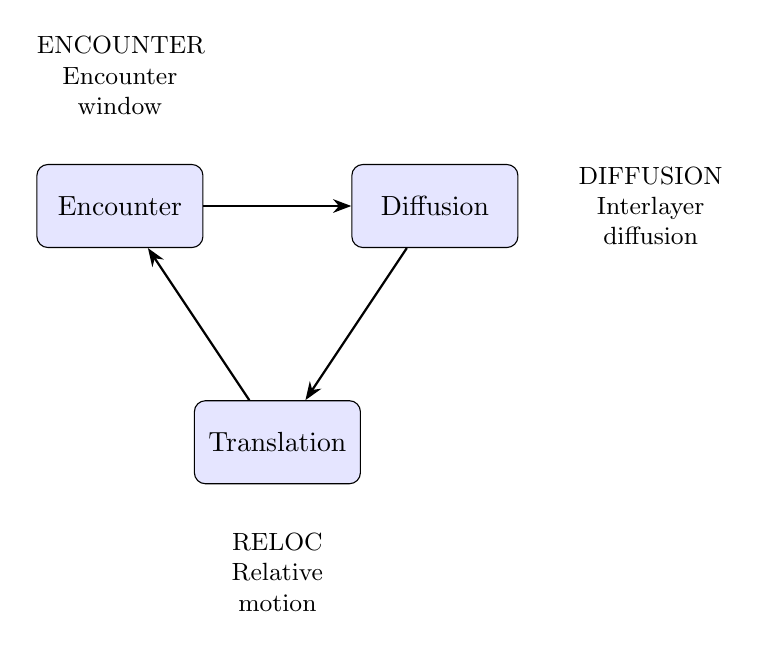
\begin{tikzpicture}[
process/.style={rectangle, rounded corners, minimum height=3em, minimum width=6em, text centered, draw=black, fill=blue!10},
arrow/.style={-Stealth, thick},
annotation/.style={text width=6em, font=\small, align=center}
]
% Define the nodes for each step (3 boxes only)
\node[process] (encounter) at (0,0) {Encounter};
\node[process] (diffusion) at (4,0) {Diffusion};
\node[process] (translation) at (2,-3) {Translation};
% Draw arrows to indicate the cyclic process (triangle shape)
\draw[arrow] (encounter) -- (diffusion);
\draw[arrow] (diffusion) -- (translation);
\draw[arrow] (translation) -- (encounter);
% Add annotations for constants
\node[annotation, above=0.5cm of encounter] (encounter-anno) {ENCOUNTER\\ Encounter window};
\node[annotation, right=0.5cm of diffusion] (diff-anno) {DIFFUSION\\ Interlayer diffusion};
\node[annotation, below=0.5cm of translation] (reloc-anno) {RELOC\\ Relative motion};
\end{tikzpicture}
\end{center}
\caption{The light frame---the period of the information clock, within which a wavefront advances exactly one lattice cell at the maximum information speed $v_{\max}$---has three stages: Encounter, Diffusion and Translation, delimited by the constants ENCOUNTER, DIFFUSION and RELOC.}
\label{fig:light_frame}
\end{figure}
\medskip\noindent\textbf{Definitions.}\label{subsec:Definitions} The frame constants of the light frame are the following:
\begin{itemize}
\item \textbf{DIAG}\\
$\lfloor\sqrt{3}\,L\rfloor$: diagonal length of the lattice; upper bound for interaction distances.
\item \textbf{RMAX}\\
$L/2$: maximum bubble radius before wrapping (the breathing-phase amplitude).
\item \textbf{ENCOUNTER}\\
$2W$: encounter window.
\item \textbf{DIFFUSION} \\
$ENCOUNTER + 2W + \lfloor\sqrt{3}(L-1)/2\rfloor + 9(L-1) + 2W$: diffusion range along $W$; also alerts all layers of an imminent collapse.
\item \textbf{RELOC}\\
$DIFFUSION + 3(L-1)$: translation phase.
\item \textbf{REISSUE}\\
$RELOC + 1$: re-emission of the wavefront from the new source center.
\item \textbf{FLOOD}\\
$REISSUE + 3(L-1)$: final synchronization of the three lattices.
\item \textbf{FRAME}\\
Same value as $FLOOD$; total duration of the light step.
\item \textbf{effective\_t}\\
Triangular breathing phase (the active-shell radius): $\mathrm{effective\_t}(t)=t\bmod L$ for $t\bmod L\le L/2$, and $L-(t\bmod L)$ otherwise.  The active-shell radius therefore advances one cell per step of the local tick $t$---i.e., per light frame---from $0$ up to the amplitude $L/2=\mathrm{RMAX}$ on the expansion branch and back to $0$ on the contraction branch; each branch lasts $L/2$ frames, so one era (one full expansion-and-contraction cycle) has period $L=2\,\mathrm{RMAX}$ in $t$ and spans $L$ light frames.  An era is distinct from a light frame and from the housekeeping tick $k$.
\end{itemize}
\subsection{Bubble, pair, singleton, and cluster} \label{subsec:pairs}
A \emph{bubble} is an expanding spherical wavefront of information organized across cells within a common layer. Spherical propagation is determined by comparing the dynamic radius $r$ to the wavefront tick $t$.
\subsubsection{Pair}
Two bubbles are overlapping if they share the same spatial coordinates and $t_1=t_2$. Overlapping bubbles can form a \emph{pair} if they have the same affinity, that is, $a_1=a_2$; the two partners share a center and phase, and their charges are complementary or matching depending on the pair's role. Pairs may remain bound to a particle as \emph{dressing} pairs or propagate freely as photons; a free pair expands outward and is gradually consumed, releasing two singletons at distinct locations.
\subsubsection{drive pair} \label{subsubsec:drive pair}
A pair can act as a \textit{drive pair}, repositioning other bubbles and providing inertia.
A drive pair is a reciprocal photon-type pair that has adopted the island's affinity $a$ and carries a non-zero transport vector $\boldsymbol{m}$, typically on the scale $L/2$. Neither a nonzero vector alone nor receiving a translation impulse makes a source a drive pair. A free pair must first acquire the particle's affinity.
\paragraph{Current experimental scope.} Revalidation with $D\times D$ promotion and $K\times K$ clash enabled confirms sustained transport of a prepared K with one drive pair in both directions. In the matched experiment, the mean displacement after the initial measurement window is one cell per light frame, with coincident pair halves and no pair departure over 96 frames. This is a journey-step result, not a universal speed measurement per housekeeping tick. Prepared multi-constituent bodies do not retain a single chief identity under the current role dynamics. The production reference retains directed motion of the prepared constituent set, while the matched K+2D case also loses spatial cohesion. These results therefore validate minimum drive-pair transport, not yet the inertia of a persistent multi-constituent island (revalidation commands and traces: \texttt{experiments/INERTIA\_REVALIDATION.md}).
Consider an island of $N=L/3$ equal charge elements, one chief $K$ and $N-1$ delegates $D$, all sharing $a$. Its $K\times D$ and $D\times D$ contacts maintain dynamic cohesion. Without drive pairs its center of mass remains at rest in the lattice frame, although its constituents may rearrange. Bound pairs supply persistent internal propulsion through $P\times K$ and $P\times D$ contacts. A rightward resultant of their transport vectors drives a rightward mean displacement of the cohesive island. Few aligned pairs give sparse kicks and low velocity; many nearly collinear pairs give more frequent coherent kicks and higher velocity, up to the lattice transport bound. This is the proposed mechanism of inertia, not an externally imposed velocity of the aggregate.
The reference simulation algorithm resolves each unordered source contact once per light frame, counting a reciprocal pair once rather than once per half or overlapping voxel. A pair can deliver at most one unit face-step to one contacted body element, in a direction selected from $\boldsymbol{m}$; receiving that step preserves the target's $K/D$ identity. $\boldsymbol{m}$ is not a displacement of $L/2$ cells and is retained while the pair remains a drive pair. These mechanical, same-affinity contacts are not gated by the electroweak sieve.
\subsubsection{Singleton}
An unpaired bubble is called a \textit{singleton}; it is not a generic synonym for bubble.
\subsubsection{cluster}
The \textit{cluster} is a group of superposed pairs having the same affinity, same true $bB$ bits and the same (active) pBits.
\subsubsection{Specialized pairs} \label{subsec:specialized-pairs}
Certain pair combinations are not allowed to form clusters:
\begin{itemize}
\item Neutrino and antineutrino pairs possess color values $N, N$ and $\bar{N}, \bar{N}$, respectively.
\item The up quark fragments $u$ exhibit equal, nontrivial colors and a positive charge in the case of Orbis.
\item The drive pair adds to the relativistic mass of the propelled fermion.\footnote{This mirrors a Kantian view: particles do not self-move but require an external cause---here, interaction with fragments---to change their state.}
\item Pairs with fully complementary charges are \emph{gravitons}. They operate in both Orbis and Umbra,\footnote{Orbis and Umbra coexist spatially.} have fixed oscillation frequency $2$, and mediate static cross-sector interactions; without them, Umbra matter would appear inert in Orbis. Graviton-induced gravity is detailed in Sect.~\ref{subsec:emergence-of-gravity}.
\end{itemize}
\subsection{Interaction principles}
The guiding principles are:
\medskip\noindent\textbf{Wavefronts clash.} The wavefronts of both bubbles must be active, i.e.\ $r_1 = \mathrm{effective\_t}(t_1)$ and $r_2 = \mathrm{effective\_t}(t_2)$, where $r_i$ is the propagated integer radius of bubble $i$ and $t_i$ is its local frame counter. This condition is assumed in all rules below.

\medskip\noindent\textbf{Aggregation and dissolution.}\label{subsec-role-of-affinity} Bubbles aggregate by sharing a common affinity; the smallest value prevails, $a_1=a_2=\min(a_1,a_2)$. On dissolution, they revert to their layer indices, $a_1=w_1$ and $a_2=w_2$. If a singleton meets a pair, the pair takes the singleton's affinity, $a_2^1=a_2^2=a_1$. The value $a=W$ marks an orphan. The idempotent $\min$ operator naturally supports an ontological model of entanglement.

\medskip\noindent\textbf{Charge conjugation.} Charge conjugation constrains interactions by requiring charge neutrality in the outcome. Electric neutrality requires a pair of opposite charges; a single bit cannot be neutral alone. Weak neutrality follows from the combination of the two weak bits in both \textit{Orbis} and \textit{Umbra}. Strong neutrality is $000$ (or $111$ for anti-neutrality); a pair with complementary color bits (e.g.\ $101$ and $010$) is also neutral. In general, interactions drive the resulting charge combination toward neutrality.

\medskip\noindent\textbf{Reciprocity.} Because only one draft can be updated at a time, the rules must later update the counterpart. This reciprocity is essential for the next subsection.
\subsection{Encounter} \label{subsec:encounter}
Encounter is the first step of the light frame (ending at $ENCOUNTER$) and contains the main interaction rules. Each site in the main lattice is compared with its partner along the $W$ dimension. This partner comparison is a rule-evaluation device that pairs lattice sites by internal address; it does not move bubbles along $W$---physical motion and merging always occur in the 3-torus (Sect.~\ref{subsec:w-islands}). During this step the wave phase $f$ (the triangular breathing phase of Sect.~\ref{sec:light-frame}) selects the wave-cloud point density at the current shell, while the notion of frequency is carried by the pair count (Sect.~\ref{bosons}). Particles form or reform here. We postulate that the weak force only causes collapse, not limited reissues. Comparisons split into two cases: superposing or distinct bubbles.
\subsubsection{Superposing bubbles}
Two overlapping bubbles with the same wavefront tick $t_1=t_2$ can form a pair if they satisfy the following conditions:
\begin{itemize}
% Rule 1
\item
$ (q_a \oplus q_b) \land (w1_a \oplus w1_b) \land (w0_a \oplus w0_b) \land (c2_a \oplus c2_b) \land (c1_a \oplus c1_b) \land (c0_a \oplus c0_b) $
\item
% Rule 2
$ (q_a \oplus q_b) \land (w1_a = w1_b) \land (w0_a \oplus w0_b) \land (c2_a \oplus c2_b) \land (c1_a \oplus c1_b) \land (c0_a \oplus c0_b) $
\item
% TODO: add the gluon and weak boson formation rules
% Rule 3
$ ch_a = ch_b = 000000\mathrm{B} $
\item
% Rule 4
$ ch_a = ch_b = 111111\mathrm{B} $
\item
% Rule 5
$ (q_a = q_b = 0) \land (w1_a = w1_b = 0) \land (w0_a = w0_b = 1) \land (color_a = color_b) \land (color_a \neq 000\mathrm{B} \land color_a \neq 111\mathrm{B}) $
\item
% Rule 6
$ (q_a = q_b = 1) \land (w1_a = w1_b = 1) \land (w0_a = w0_b = 0) \land (color_a = color_b) \land (color_a \neq 000\mathrm{B} \land color_a \neq 111\mathrm{B}) $
\end{itemize}
To make the six rules concrete, Table~\ref{tab:charge-examples} in Appendix~\ref{app:charge-examples} lists representative bit-strings and the pairs they form (the bit order $w_{1}\,w_{0}\,q\,c_{2}\,c_{1}\,c_{0}$ and the color code follow Table~\ref{tab:Cell-structure}).
These rules implement the formation of pairs, as defined in Sect. \ref{subsec:pairs}.
If pairs are detected, one frequency unit is registered on the pair stack (Sect.~\ref{bosons}); the wave phase $f$ itself remains the triangular breathing phase of the local tick.
$s2B$ is updated as $s2B' = s2B \ \textbf{and} \ \mathit{active}$.
Notice that the pairs are formed in two steps: first, cell $a$ compares with cell $b$, and later, cell $b$ compares with cell $a$ (reciprocity).
The formation of clusters is made during this step too, also following the reciprocity principle.
Pairs are allowed to superpose if they are equal and were formed by the two first rules above.
\subsubsection{Distinct bubbles} \label{subsec:distinct}
The $w_1$ bit separates distinct-bubble interactions into same-sector ($w_1^1=w_1^2$) and inter-sector cases; we first treat same-sector interactions.

If two same-sector singletons have opposite charges and both $kB$ bits false, we have annihilation, with both bubbles being reissued from the contact point and their affinity receiving their default values. The draft $kB$ bit turns true, triggering a collapse.
Else if two singletons have the same charge, we have fermion cohesion.
One bubble is reissued from the contact point, while the other, from its active $sB$ site.
Also, they become entangled ($a_1=a_2$).

On the other hand, if the two bubbles share the same affinity, but have different charges, the bubble whose wavefront at the contact point has $pB=1$ is reissued from the contact point.
For bound $P\times K/D$ transport, the pushing pair's $\boldsymbol{m}$ selects a unit step accumulated in $\boldsymbol{\mathit{reloc}}$, as specified in Sect.~\ref{subsec:translation}; copying the full magnitude of $\boldsymbol{m}$ as a displacement is not the inertial rule. The following contact-site reissue description concerns the other interaction channels.
That is, one bubble is reissued from $\boldsymbol{x1}$, while the other from $(\boldsymbol{x_1}-\boldsymbol{x_2})\,\boldsymbol{mod}\,L$.

For color-neutral combinations there are two cases: gluon$\times$gluon and quark$\times$gluon.
In both cases, the two bubbles are reissued from the contact point and the partners colors are exchanged.

In the electroweak sector, both $\mathit{active}$ bits must be true; together with $s2B$ they determine the harmonic behavior. This sieve mechanism applies only to electroweak interactions and helps explain why the strong force is stronger.
The weak interaction occurs when the weak charges are combined to neutrality and either ($pB_1=1$, $pB_2=0$) or ($sB_1=sB_2=1$); it always triggers collapse ($kB=1$).
The electric case uses one $pB$ bit, the magnetic case one $sB$ bit. If both $pB$ bits are true (or both $sB$ bits in the magnetic case), a collapse is triggered ($kB=1$).
If only one $pB$ bit meets the other's surface, the interaction is adiabatic: no collapse occurs, but the bubbles exchange affinity and time and relocate to each other's center. The $a$ and $t$ values then spread throughout the layer.

At the initial singularity, all bubbles overlap. If two bubbles belong to different sectors and $t=RMAX/2$, they are reissued from their active $pB$ and $sB$ sites, dispersing the singularity and separating Orbis from Umbra. We call this \textit{dispersion}.
\subsubsection{Inter-sector interactions}
For inter-sector interactions, fully complementary charges lead to \textit{singularization}; otherwise the electroweak rules above apply. Singularization is the counterpart to dispersion.
The bubbles are reissued from the contact point ($pB_{curr}=\text{true}$).
%%% DIFFUSION %%%
\subsection{Diffusion, translation and collapse in one reading}\label{subsec:translation}
Three coupled tasks close the frame---diffusion, translation, and collapse handling---and are described together because they share the same coordination state.

Diffusion propagates the information needed for translation, ending at the \texttt{DIFFUSION} tick (Figure~\ref{fig:diffusion}). If any collapse bit $kB$ is set, it spreads to all bubbles sharing the same affinity, identifying every contributor to the collapsing particle.

The wave phase $f$ is not diffused: it is the local triangular breathing phase $\mathrm{effective\_t}(t)$ of each cell (Sect.~\ref{sec:light-frame}). Phases incremented by multiples of the era period interact with the wave-cloud sieve to form concentric bubbles; the active wavefront point ($t=d$) is forwarded to the Euclidean bubble through $s2B$.

At the same time, the translation vector $\mathbf{c}$ diffuses through the layer: each cell copies the first non-trivial $\mathbf{c}$ found among its neighbors. Finally, $sB$ homing increments $\boldsymbol{c}$ along any axis where a neighbor has $homB=1$, but only when the local cell has $sB=0$. By the end of diffusion, $\boldsymbol{c}$ is ready for translation.
\begin{figure}
\begin{center}
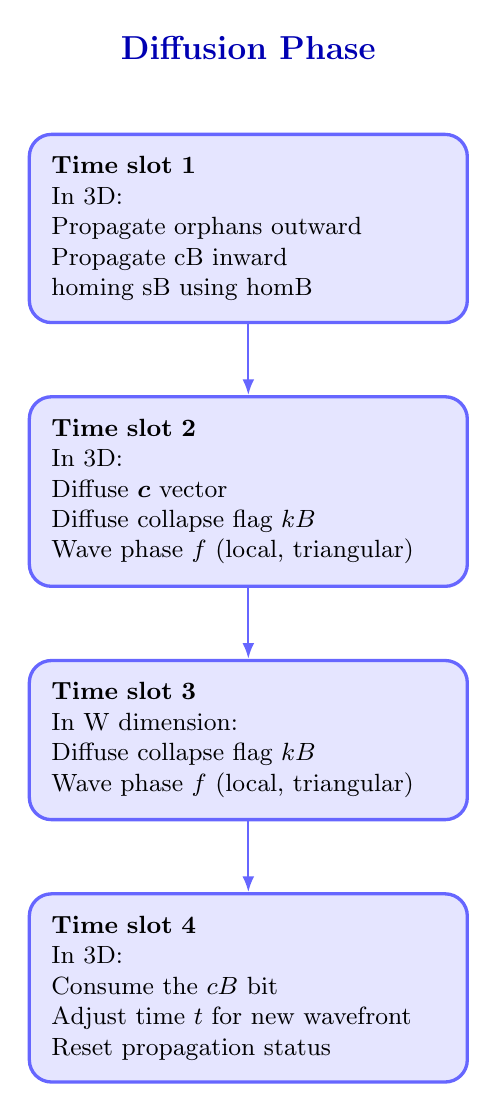
\begin{tikzpicture}[
every node/.style={font=\small, align=left},
phase/.style={rectangle, rounded corners=8pt, draw=blue!60, fill=blue!10, very thick, text width=5cm, inner sep=8pt},
arrow/.style={-{Latex[length=2mm]}, thick, blue!60}
]
% Nodes (closer spacing)
\node[phase] (t1) {
\textbf{Time slot 1}\\
In 3D:\\
Propagate orphans outward\\
Propagate cB inward\\
homing sB using homB
};
\node[phase, below=0.9cm of t1] (t2) {
\textbf{Time slot 2}\\
In 3D:\\
Diffuse $\boldsymbol{c}$ vector\\
Diffuse collapse flag $kB$\\
Wave phase $f$ (local, triangular)
};
\node[phase, below=0.9cm of t2] (t3) {
\textbf{Time slot 3}\\
In W dimension:\\
Diffuse collapse flag $kB$\\
Wave phase $f$ (local, triangular)
};
\node[phase, below=0.9cm of t3] (t4) {
\textbf{Time slot 4}\\
In 3D:\\
Consume the $cB$ bit\\
Adjust time $t$ for new wavefront\\
Reset propagation status
};
% Shorter arrows
\draw[arrow] (t1.south) -- ++(0,-0.25) -> (t2.north);
\draw[arrow] (t2.south) -- ++(0,-0.25) -> (t3.north);
\draw[arrow] (t3.south) -- ++(0,-0.25) -> (t4.north);
% Title
\node[above=0.8cm of t1, font=\bfseries\large, blue!70!black] {Diffusion Phase};
\end{tikzpicture}
\end{center}
\caption{The Diffusion phase is composed of several time slots. It spreads all information necessary for translation.}
\label{fig:diffusion}
\end{figure}
%%% Translation %%%
\medskip\noindent\textbf{Translation.} This part of the light step addresses bubble translation itself, building on the diffusion step.
It ends at the RELOC tick. Bubbles shift in specific directions (north, west, down) until they have completed their translation process, including the inertial transport mechanism.

The example rule is: if $\textbf{c}_x^{north}>0$, copy the content of the neighbor cell to the draft cell and decrement $\textbf{c}_x$ at the draft cell.
Since wavefront propagation is guided by the dynamic radius $r$ propagated from the source cell, when a bubble is re-emitted due to interaction with other bubbles, all pertinent cell information must be shifted, or relocated, to the new position determined by the variable $\textbf{c}$.
This ensures that the bubbles are relatively displaced from each other.
The final operation sets $t=0$ at the center cell of the relocated pattern.

Translation is the main consequence of an interaction.
Bubbles are re-emitted either immediately after an interaction or through wrapping.
When the bubble is reissued, the previous wavefront continues to propagate until it fades through wrapping.

In this state, the bubble is referred to as an \textit{orphan}, meaning it has affinity disabled but is still capable of non-collapsing interactions.
In this case, $a=W$ for the outer cells, set during the translation step.

To complete, the diffusion of the time variable $t$ occurs here at the last tick: When a cell has a neighboring cell with a lower $t$ value, it updates its own $t$ variable to match the lower value.
With this rule, the relocated bubble is capable of expanding again.
This timing is crucial to avoid the 'clean diamond' pattern with the new values overrunning the orphaned data.

When the translation is complete, bubble variables are prepared for the next cycle.
If the time frame completes, the $k$ counter resets to zero, preparing the system for the next iteration.
At the conclusion of the process, all $\boldsymbol{c}$ vectors will have a null value.

For internal inertial transport, source contacts are gathered during the encounter window and resolved at the end of the light frame. The numerical experiments use the following operational choices to evaluate the proposed transport mechanism. Reciprocal $K\times D$ and $D\times D$ face-steps reduce separations greater than one cell without changing the sum of body positions. Each body element can move at most once per frame. Each reciprocal drive pair pair can push at most one contacted body element; among eligible contacts it prefers the rear element along $\boldsymbol{m}$, with a rotating address tie-break. An integer DDA distributes successive face-steps in proportion to the absolute components of $\boldsymbol{m}$, retaining their signs. Zero-radius phases have no extended propelling surface. Both halves of the bound pair recycle by the same bounded face-step toward the contacted constituent. These are reference transport rules to test the proposed mechanism, not a derivation of Newtonian mechanics or rotational invariance.

The resulting unit step, rather than the full vector $\boldsymbol{m}$, enters $\boldsymbol{\mathit{reloc}}$. At the frame boundary, \texttt{applyMomentum} translates the bubble's layer state periodically, consumes the step and preserves its charge, affinity, source kind, pair identity, clock and transport vector. Translating the distance field together with its source avoids leaving a false source or stale distance minima. The source transaction commits after the voxel sweep so later cells cannot overwrite previously registered contacts or source changes. The partner rotation selects a $W$ identity; active flags are read at the current physical instant rather than from the preceding frame's shell.
The simulation algorithm uses globally coordinated source snapshots, contact arbitration, and layer translations. A strictly local cellular realization of that coordination remains to be established; the mechanical tests below validate the reference algorithm, not the purity constraints of Sect.~\ref{subsec:purity}. Dynamic initialization is never suspended, but election does not overwrite the direction of an already bound drive pair.
Let $N$ denote the number of equal $K/D$ body elements, excluding the drive pair dressing. For $n$ successful collinear unit kicks in a frame, with reciprocal cohesion contributing zero net displacement, the body's mean center of mass advances by
\begin{equation}
\Delta_{\mathrm{CoM}} \;=\; \frac{n}{N}
\end{equation}
cells per frame, with $n \leq N$. Oppositely directed steps enter with their signs; for general directions use $N^{-1}\sum_i\Delta\boldsymbol{x}_i$. This is a measured displacement identity, not a velocity assigned to the island or a mass law. drive pair-pair centers must be counted once each when separately measuring the dressed particle. Without propulsion, reciprocal cohesion preserves the body's center of mass. The displacements reported here are measured in cells per light frame. The housekeeping counter $k$ indexes the internal stages of that frame and is not the physical time used in these measurements.
Non-drive pair pairs behave differently: in $K \times K$ or $D \times D$ between different tribes the source centers move one light-step away from each other, exchanging momentum through $\boldsymbol{\mathit{reloc}}$.

An unbound pair may acquire an island's affinity through an admissible encounter. Subsequent same-affinity contacts provide propulsion; a pair of a different affinity cannot act as that island's internal drive pair. Receiving a displacement never promotes a $K/D$ source to $P$.
\medskip\noindent\textbf{Annihilation and collapse.} Annihilation and light-matter collapse both occur during the encounter stage. In annihilation, the affinity reverts to its default value $a=w$, and the resulting bubbles become raw material for new particles.
This ontological collapse introduces an arrow of time at the fundamental level, reinforcing the second law of thermodynamics and pushing Poincar\'{e} recurrence far into the future (Sect.~\ref{sec-undecidability}).
\paragraph{Reversibility.} Because Fredkin and Margolus are cited as bases (Sect.~\ref{sec:related-work}), the reversibility status should be stated explicitly.  The transition is \emph{not} injective: (i) the $s2B$ sieve discards information (the gate result is a single bit derived from a product modulo $S$); (ii) collapse sets $kB$ and reverts affinity to its default, and reissue resets the local clock $t$; (iii) relocation moves source centers and the flood stage synchronizes the three lattices by overwrite.  Each of these steps is many-to-one, so the map from one light frame to the next is not reversible, and no inverse step is defined.  This is a deliberate difference from Fredkin's reversible-computation program: the model is a dissipative deterministic automaton with an explicit arrow of time (see above), and it is not a candidate for Landauer-free computation.  The claim is that the irreversible steps are confined to the hidden coordination fields and to the aggregate bookkeeping, so that the \emph{physical} (readable) evolution keeps its local, causal character (Sect.~\ref{subsec:nosignaling-formal}); reversibility of the whole map is neither assumed nor required.
\subsection{Main lattice updating and partner refresh} \label{subsec:updating}
At the end of each $k$ tick, the draft lattice is transferred to main. If $k$ lies inside the $ENCOUNTER$ window, draft is first shifted along $W$ to enable encounter. This shift is a cyclic permutation of internal addresses for evaluation, not propagation of bubbles along an extra spatial axis---all physical motion remains confined to the 3-torus (Sect.~\ref{subsec:w-islands}). The partner lattice is then refreshed from main so the next encounter can compare main and partner along $W$; it copies the wave phase and active flag, $f_i^{partner}=f_i^{main}$ and $\mathit{active}_i^{partner}=\mathit{active}_i^{main}$.
\begin{figure}[ht]
\centering
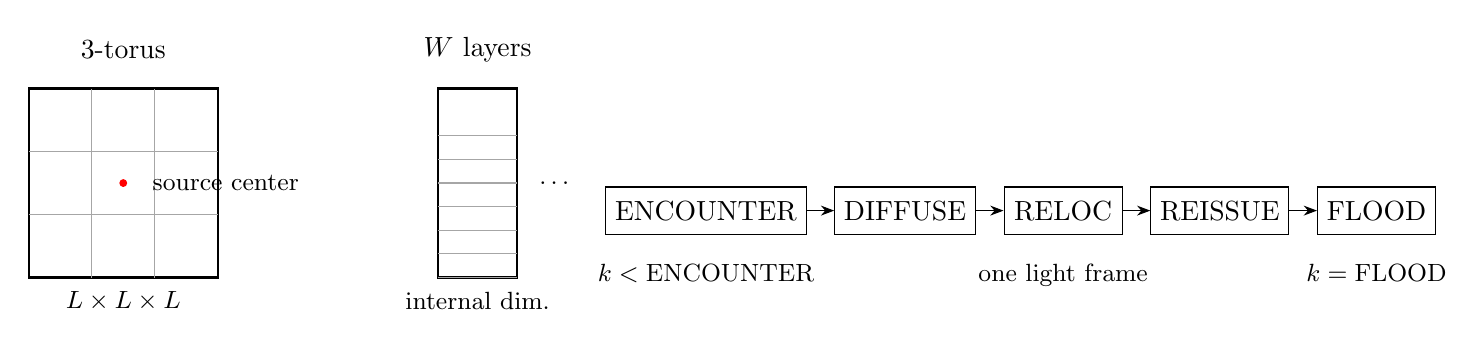
\begin{tikzpicture}[node distance=1.1cm, >=Stealth]
% --- 3-torus ---
\draw[thick] (0,0) rectangle (2.4,2.4);
\draw[gray!70] (0,0.8) -- (2.4,0.8);
\draw[gray!70] (0,1.6) -- (2.4,1.6);
\draw[gray!70] (0.8,0) -- (0.8,2.4);
\draw[gray!70] (1.6,0) -- (1.6,2.4);
\node at (1.2,2.9) {3-torus};
\node[font=\small] at (1.2,-0.3) {$L\times L\times L$};
\filldraw[red] (1.2,1.2) circle (1.2pt);
\node[font=\small, right] at (1.45,1.2) {source center};
% --- W stack ---
\begin{scope}[xshift=5.2cm]
\draw[thick] (0,0) rectangle (1.0,2.4);
\foreach \i in {0,1,2,3,4,5,6} {
\draw[gray!70] (0, 0.3*\i+0.0) -- (1.0, 0.3*\i+0.0);
}
\node at (0.5,2.9) {$W$ layers};
\node[font=\small] at (0.5,-0.3) {internal dim.};
\node[font=\small] at (1.5,1.2) {$\dots$};
\end{scope}
% --- light-frame pipeline ---
\begin{scope}[xshift=8.6cm, yshift=0.85cm]
\node[draw, rectangle, minimum width=1.5cm, minimum height=0.6cm] (c1) {ENCOUNTER};
\node[draw, rectangle, minimum width=1.5cm, minimum height=0.6cm, right=0.35cm of c1] (c2) {DIFFUSE};
\node[draw, rectangle, minimum width=1.5cm, minimum height=0.6cm, right=0.35cm of c2] (c3) {RELOC};
\node[draw, rectangle, minimum width=1.5cm, minimum height=0.6cm, right=0.35cm of c3] (c4) {REISSUE};
\node[draw, rectangle, minimum width=1.5cm, minimum height=0.6cm, right=0.35cm of c4] (c5) {FLOOD};
\draw[->] (c1) -- (c2);
\draw[->] (c2) -- (c3);
\draw[->] (c3) -- (c4);
\draw[->] (c4) -- (c5);
\node[font=\small, below=0.25cm of c1] {$k<\mathrm{ENCOUNTER}$};
\node[font=\small, below=0.25cm of c3] {one light frame};
\node[font=\small, below=0.25cm of c5] {$k=\mathrm{FLOOD}$};
\end{scope}
\end{tikzpicture}
\caption{Model architecture. \label{fig:architecture} Left: the $L\times L\times L$ 3-torus (spatial fabric), with one source center per layer emitting a spherical wavefront.  Middle: the internal dimension of $W$ layers; each layer carries one bubble and the layers are compared by the encounter stage.  Right: the light-frame pipeline of the finite-state machine---\textsc{Encounter} (interaction rules), diffusion of affinity and flags, relocation of sources, reissue, and flood---executed in $\mathrm{FRAME}$ housekeeping ticks $k$; the wavefront advances exactly one cell per tick, at the maximum information speed $v_{\max}$.}
\end{figure}
\subsection{Algorithmic summary of one light frame}\label{subsec:algorithm}
For reproducibility, Algorithms~\ref{alg:lightframe}--\ref{alg:cluster} give a self-contained account of one complete light frame: Algorithm~\ref{alg:lightframe} is the frame driver (incremental distance field, integer wave update, the six interaction stages, the charge-conjugation hook, momentum and lattice swap), and Algorithms~\ref{alg:pair}--\ref{alg:cluster} give the interaction rules invoked by the \textsc{Encounter} stage.  Together they define the full transition function; the repository (Ref.~\cite{af_neto}, \texttt{simulation.cpp}, \texttt{interaction.cpp}) is not needed to reproduce the dynamics.  The notation follows Table~\ref{tab:Cell-structure}: a charge word is written $w_{1}\,w_{0}\,q\,c_{2}\,c_{1}\,c_{0}$ (most significant first), $c_{2}c_{1}c_{0}$ is the color, $000\mathrm{B}=N$ and $111\mathrm{B}=\bar{N}$, and $\overline{ca}$ denotes the six-bit complement of the charge word $ca$.  Subscripts $a$ and $b$ label the two interacting bubbles, so $q_a$ is bit $q$ of bubble $a$, $w_{1,a}$ bit $w_{1}$ of bubble $a$, and so on.
\begin{algorithm}[ht]
\caption{One complete light frame (the full per-cell transition function, one synchronous $k$-tick).}
\label{alg:lightframe}
\begin{algorithmic}[1]
\Require $L$, $W=3L^{2}$, $\mathrm{RMAX}=L/2$, and the stage bounds
$\mathrm{ENCOUNTER}<\mathrm{GSLOT\_Z}<\mathrm{DIFFUSION}<\mathrm{RELOC}<\mathrm{REISSUE}<\mathrm{FLOOD}=\mathrm{FRAME}$ (Sect.~\ref{subsec:Definitions});
the housekeeping tick $k$, the wavefront tick $t$, and the wave phase $f=\mathrm{effective\_t}(t)$ are the cell fields of Table~\ref{tab:Cell-structure}
\Ensure the three lattices advanced by one light step
\Procedure{LightFrame}{}
\State \Call{UpdatePulsatingWavefront}{} \Comment{incremental distance field: radii $r^{2},r$ from the moving source center by $\Delta{=}2a{+}1$ increments, no square roots}
\State $pulse\_tick \gets pulse\_tick + 1$
\State \Call{PhaseStep}{} \Comment{integer wave update $v \gets v + (\nabla^{2}u \gg s)$, $u \gets u + v$, damping $v \gets v - (v \gg s_{d})$, shifts $s,s_{d}$ radius-dependent; hard zero outside the sphere; $active \Leftrightarrow r=\mathrm{effective\_t}(t)$}
\State swap $lattice\_curr \leftrightarrow lattice\_draft$
\State \Call{PolarizationTick}{} \Comment{elected-momentum broadcast over the $W$-ledger; stamps arrival ticks $b(x)$}
\For{$w = 0 \ldots W{-}1$} \Comment{loop over the internal dimension}
\For{each cell $(x,y,z)$ in the 3-torus}
\State $C \gets lattice\_curr(x,y,z,w)$; $D \gets C$; $M \gets lattice\_partner(x,y,z,w)$ \Comment{$M$: the partner cell}
\If{$k < \mathrm{ENCOUNTER}$}
\State \Call{Encounter}{$C,D,M$} \Comment{interaction rules R1--R6, Algorithms~\ref{alg:pair}--\ref{alg:cluster}; source-kind (K/S/D/P) contact re-emission and momentum impulse}
\ElsIf{$k < \mathrm{GSLOT\_Z}$}
\State glider slots \Comment{reserved for the antipodal transport schedule; not exercised by the reference simulation algorithm}
\ElsIf{$k < \mathrm{DIFFUSION}$}
\State \Call{Diffuse}{$C,D$} \Comment{orphan expansion ($a \gets W$ from a full neighbor); homing $homB \to$ translation vector $\boldsymbol{c}$; $\boldsymbol{c}$ and $kB$ transport; affinity settle}
\ElsIf{$k < \mathrm{RELOC}$}
\State \Call{Relocate}{$C,D$} \Comment{consume the translation vector $\boldsymbol{c}$ along the three axes (north, west, down)}
\ElsIf{$k < \mathrm{REISSUE}$}
\State \Call{Reissue}{$C,D$} \Comment{reset $kB,homB,bB$; propagate affinity outward from $active$ cells; consume the contraction flag $cB$ (reset $t$)}
\Else
\State \Call{Flood}{$C,D$} \Comment{synchronize the light clock: $D.t \gets \min$ of the six neighbor $t$}
\EndIf
\State $D.k \gets (C.k + 1) \bmod \mathrm{FRAME}$
\If{$D.k = 0$} \Comment{a new light frame begins}
\State $D.t \gets (C.t + 1) \bmod (2\,\mathrm{RMAX})$ \Comment{island cells ($a{=}W$, $t \le \mathrm{RMAX}$) count without the modulus}
\EndIf
\EndFor
\EndFor
\State \Call{ApplyChargeConjugation}{} \Comment{matter--antimatter turnaround hook; exact no-op when the bias $\varepsilon = 0$}
\State \Call{CommitSourceTick}{} \Comment{commit source changes; on the frame boundary resolve unique internal contacts}
\State \Call{ApplyMomentum}{} \Comment{consume free photon pairs at turnaround; translate layer states by pending steps, preserving bound-pair identity and $\boldsymbol{m}$}
\State \Call{SwapLattices}{} \Comment{$\mathrm{draft}\to\mathrm{curr}$; at $k=0$ refresh the partner ($M.f \gets \mathrm{effective\_t}(M.t)$); while $k<\mathrm{ENCOUNTER}$ rotate the partner $W$-slices (\textsc{RotatePartners})}
\EndProcedure
\end{algorithmic}
\end{algorithm}
\begin{algorithm}[ht]
\caption{Exact interaction rules for the six charge bits (superposing bubbles).}
\label{alg:pair}
\begin{algorithmic}[1]
\Function{CanFormPair}{$a,b$}
\State $ca \gets a.ch$; $cb \gets b.ch$
\If{$ca = 000000\mathrm{B}$ \textbf{and} $cb = 000000\mathrm{B}$} \Comment{R3: neutrino}
\State \Return \textbf{true}
\ElsIf{$ca = 111111\mathrm{B}$ \textbf{and} $cb = 111111\mathrm{B}$} \Comment{R4: antineutrino}
\State \Return \textbf{true}
\ElsIf{$\overline{ca} = cb$} \Comment{R1: graviton, all six bits complementary}
\State \Return \textbf{true}
\EndIf
\State $(q_a,w_{1,a},w_{0,a}) \gets$ decode bits of $ca$; $(q_b,w_{1,b},w_{0,b}) \gets$ decode bits of $cb$
\State $col_a \gets ca \& 111\mathrm{B}$; $col_b \gets cb \& 111\mathrm{B}$
\If{$q_a \neq q_b$ \textbf{and} $w_{1,a} = w_{1,b}$ \textbf{and} $w_{0,a} \neq w_{0,b}$ \textbf{and} $col_a \oplus col_b = 111\mathrm{B}$} \Comment{R2: gluon}
\State \Return \textbf{true}
\ElsIf{$q_a = q_b = 0$ \textbf{and} $w_{1,a} = w_{1,b} = 0$ \textbf{and} $w_{0,a} = w_{0,b} = 1$ \textbf{and} $col_a = col_b$ \textbf{and} $col_a \notin \{000,111\}\mathrm{B}$} \Comment{R5: up quark}
\State \Return \textbf{true}
\ElsIf{$q_a = q_b = 1$ \textbf{and} $w_{1,a} = w_{1,b} = 1$ \textbf{and} $w_{0,a} = w_{0,b} = 0$ \textbf{and} $col_a = col_b$ \textbf{and} $col_a \notin \{000,111\}\mathrm{B}$} \Comment{R6: up quark}
\State \Return \textbf{true}
\EndIf
\State \Return \textbf{false}
\EndFunction
\end{algorithmic}
\end{algorithm}
\begin{algorithm}[ht]
\caption{cluster formation, electric/magnetic channels, and collapse (superposing and distinct bubbles).}
\label{alg:cluster}
\begin{algorithmic}[1]
\Function{CanFormcluster}{$a,b$}
\State $ca \gets a.ch$; $cb \gets b.ch$
\If{$ca = cb = 000000\mathrm{B}$ \textbf{or} $ca = cb = 111111\mathrm{B}$} \Comment{R3/R4 never cluster}
\State \Return \textbf{false}
\ElsIf{$\overline{ca} = cb$} \Comment{R1 graviton never clusters}
\State \Return \textbf{false}
\EndIf
\State decode $(q,w_{1},w_{0})$ and $col$ of $ca,cb$ as in Algorithm~\ref{alg:pair}
\If{$q_a = q_b$ \textbf{and} $w_{1,a} = w_{1,b}$ \textbf{and} $w_{0,a} = w_{0,b}$ \textbf{and} $col_a = col_b$ \textbf{and} $col_a \notin \{000,111\}\mathrm{B}$} \Comment{R5/R6 up quark never clusters}
\State \Return \textbf{false}
\ElsIf{$a.\mathit{reloc} \neq 0$ \textbf{or} $b.\mathit{reloc} \neq 0$} \Comment{drive pair never clusters}
\State \Return \textbf{false}
\EndIf
\State \Return $w_{1,a} = w_{1,b}$ \textbf{and} $q_a \neq q_b$ \textbf{and} $w_{0,a} \neq w_{0,b}$ \textbf{and} $col_a \oplus col_b = 111\mathrm{B}$ \Comment{only the R2 geometry}
\EndFunction
\Procedure{Encounter}{$C,D,M$}
\State $samePos \gets C.x = M.x$; $sameT \gets C.t = M.t$
\If{$samePos$ \textbf{and} $sameT$ \textbf{and} \Call{CanFormPair}{$C,M$}}
\State $D.kind \gets M.kind \gets P$; $D.pair\_idx \gets M.w$; $M.pair\_idx \gets C.w$ \Comment{form a pair}
\State $D.a \gets M.a \gets$ shared affinity; \Call{ReemitAtContact}{$D,M$}; reset $t$
\If{$newCount > 1$ \textbf{and} \Call{CanFormcluster}{$C,M$} \textbf{and} $C.pB = M.pB$ \textbf{and} $C.sB = M.sB$ \textbf{and} $C.bB = M.bB$}
\State $D.bB \gets M.bB \gets \textbf{true}$ \Comment{cluster}
\EndIf
\ElsIf{$C.pB$ \textbf{or} $M.pB$ \textbf{or} $C.sB$ \textbf{or} $M.sB$} \Comment{electric/magnetic contact}
\If{$C.pB \wedge M.pB$ \textbf{or} $C.sB \wedge M.sB$} \Comment{collapse}
\State $D.kB \gets D.cB \gets \textbf{true}$ \Comment{triggers reissue}
\Else
\State \Call{AdiabaticExchange}{$C,D,M$} \Comment{exchange affinity and phase, relocate to partner center}
\EndIf
\EndIf
\EndProcedure
\end{algorithmic}
\end{algorithm}
As given in Sect.~\ref{subsec:updating}, \textsc{SwapLattices} transfers the draft to the main lattice at the end of every $k$ tick; at $k=0$ the partner is refreshed from main (so the next encounter compares main and partner along $W$), and while $k<\mathrm{ENCOUNTER}$ the partner $W$-slices are rotated by \textsc{RotatePartners} to schedule the cross-layer adjacency.
%%%%%%%% INTERACTIONS %%%%%%%%%%
\section{Interactions\label{sec:Interactions}}
Some interaction details are now clarified.
\subsection{Charge driven interactions}
\subsubsection{Static interactions}
A static interaction (Coulomb or magnetic) between two distant charges $q_1$ and $q_2$ begins when an orphan singleton from $q_1$ aligns with a vacuum graviton; both are reissued at the contact point. If the graviton then interacts with $q_2$, it is reissued there and acquires $q_2$'s affinity. Thus gravitons propagate along the flux of orphans from particle 1, increasing the chance of hitting $q_2$ and becoming one of its drive pairs. The same occurs in reverse.
\subsubsection{Coulomb interaction} \label{subsec:Coulomb-interaction}
The proposed Coulomb mechanism involves orphan wavefronts guiding free pairs toward another particle. A pair becomes that particle's drive pair only after acquiring its affinity; subsequent internal contacts can then transport its $K/D$ constituents in the pair's $\boldsymbol{m}$ direction. The receiving constituent does not become a drive pair. The current internal-transport tests do not establish the external capture rates, charge-sign dependence or a Coulomb distance law.
\subsubsection{Static magnetic interaction}
The magnetic case uses $sB$ instead of $pB$ and applies to charged leptons, quarks and W bosons. Because drive pairs emphasize $pB$ over $sB$, fast particles tend to acquire a component perpendicular to their direction of motion.
\subsubsection{Neutrino interactions}
Let $q_{0,1}$ be a complementary electric-bit pair. A neutrino fragment has charge content $q_{0,1}=00000B$; an antineutrino has $q_{0,1}=01111B$. (Anti)neutrino fragments interact only with (right-)left-handed particles.
\subsubsection{The up quark and down quark fragments}
The color combinations of fragment pairs are shown in Table~\ref{tab:color-combination}.
(Anti)\emph{quark} fragments have non-trivial color and are marked as $1q$ or $1\bar{q}$, (anti)neutrinos are $\nu$ and $\bar{\nu}$, gluons are $g$, and photons are $\gamma$.
Since half the gluon fragments are right-handed, they are shown as photons.
The shaded cells (same-color pairs) with both quarks carrying electric charge $q=+$ may form an \emph{up quark} fragment.
An \emph{up quark} $u$ can be any of the \emph{+R+R}, \emph{+G+G} or \emph{+B+B} pairs, while a \emph{down quark} $d$ can be any of the \emph{-R}, \emph{-G} or \emph{-B} single fragments. A proton fragment \emph{uud} has an uncompensated color, balanced dynamically by the matter and antimatter ends of gluons. Hence the \emph{electron} fragment must be $-N,-N,-N$.\footnote{This explains fractional quark charges.}
The number of up-quark fragments in each sector sets an upper limit on proton, and hence \textit{atom}, production.
\subsection{Self-interference\label{subsec:Interference}}
Space in this model retains a memory of particle trajectories, producing self-interference reminiscent of the double-slit experiment \cite{feynman-2}. The trace is encoded by the last affinity value $a$ and the most recent wave phase $f$ left in visited cells.
During encounter (Sect.~\ref{subsec:encounter}), incoming and residual bubbles are compared. If $d=t$, standard cohesion occurs; if $d=f$, only the new bubble is reissued, altering the fermion's dynamics and creating interference patterns. This temporally shifted interaction among the constituent ``bits'' of qubits (Sect.~\ref{subsection:qubits}) provides a substrate for complex quantum behavior in a discrete framework.
\begin{table}[p]
\centering
\setlength{\tabcolsep}{2.2pt}
\renewcommand{\arraystretch}{0.95}
\resizebox{0.72\linewidth}{!}{%
\begin{tabular}{|c|c|c|c|c|c|c|c|c|}
\hline
&
\hdr{N}{000} &
\hdr{R}{001} &
\hdr{G}{010} &
\hdr{$\bar{\mathrm{B}}$}{011} &
\hdr{B}{100} &
\hdr{$\bar{\mathrm{G}}$}{101} &
\hdr{$\bar{\mathrm{R}}$}{110} &
\hdr{$\bar{\mathrm{N}}$}{111} \\
\hline
% N 000
\hdr{N}{000} &
\C{\nu} &
\Csec{1q}{1\ell} &
\Csec{1q}{1\ell} &
\Csec{1\overline{q}}{1\ell} &
\Csec{1q}{1\ell} &
\Csec{1\overline{q}}{1\ell} &
\Csec{1\overline{q}}{1\ell} &
\C{\gamma} \\
\hline
% R 001
\hdr{R}{001} &
\Csec{1\ell}{1q} &
\Cb{2q} &
\C{2q} &
\C{\gamma} &
\C{2q} &
\C{\gamma} &
\C{\gamma} &
\Csec{1\overline{\ell}}{1q} \\
\hline
% G 010
\hdr{G}{010} &
\Csec{1\ell}{1q} &
\C{2q} &
\Cb{2q} &
\C{g} &
\C{2q} &
\C{\gamma} &
\C{\gamma} &
\Csec{1\overline{\ell}}{1q} \\
\hline
% B-bar 011
\hdr{$\bar{\mathrm{B}}$}{011} &
\Csec{1\ell}{1\overline{q}} &
\C{g} &
\C{g} &
\Cy{2\overline{q}} &
\C{g} &
\C{2\overline{q}} &
\C{2\overline{q}} &
\Csec{1\overline{\ell}}{1\overline{q}} \\
\hline
% B 100
\hdr{B}{100} &
\Csec{1\ell}{1q} &
\C{2q} &
\C{2q} &
\C{g} &
\Cb{2q} &
\C{\gamma} &
\C{\gamma} &
\Csec{1\overline{\ell}}{1q} \\
\hline
% G-bar 101
\hdr{$\bar{\mathrm{G}}$}{101} &
\Csec{1\ell}{1\overline{q}} &
\C{g} &
\C{g} &
\C{2\overline{q}} &
\C{\gamma} &
\Cy{2\overline{q}} &
\C{2\overline{q}} &
\Csec{1\overline{\ell}}{1\overline{q}} \\
\hline
% R-bar 110
\hdr{$\bar{\mathrm{R}}$}{110} &
\Csec{1\ell}{1\overline{q}} &
\C{g} &
\C{g} &
\C{2\overline{q}} &
\C{\gamma} &
\C{2\overline{q}} &
\Cy{2\overline{q}} &
\Csec{1\overline{\ell}}{1\overline{q}} \\
\hline
% N-bar 111
\hdr{$\bar{\mathrm{N}}$}{111} &
\C{\gamma} &
\Csec{1q}{1\overline{\ell}} &
\Csec{1q}{1\overline{\ell}} &
\Csec{1\overline{q}}{1\overline{\ell}} &
\Csec{1q}{1\overline{\ell}} &
\Csec{1\overline{q}}{1\overline{\ell}} &
\Csec{1\overline{q}}{1\overline{\ell}} &
\C{\bar{\nu}} \\
\hline
\end{tabular}%
}
\caption{Color combination (rows $\times$ columns = the two fragment colors). \label{tab:color-combination}
Legend: $1q$ = one quark, $1\ell$ = one lepton, $2q$ = a quark pair (up quark), $\nu$ = neutrino, $\gamma$ = photon and $g$ = gluon; a bar denotes the antiparticle ($1\bar{q}$ = antiquark, $1\bar{\ell}$ = antilepton, $\bar{\nu}$ = antineutrino). Since half the gluon fragments are right handed, they are shown as photons. The shaded cells mark the same-color pairs that, with electric charge $q=+$, may form an \emph{up quark} fragment in Orbis (cyan, matter colors) and its anti-up (yellow, antimatter colors).}
\end{table}
%%%%%%%% PARTICLES %%%%%%%%%%
\section{Dynamic charge quantization and the scaling of $W$}\label{sec:dynamic-charge-quantization}
This section expands Sect.~\ref{subsec:w-islands} and details the dynamic organization and quantization of $W$-islands.
\subsection{Objects and identity}
A \emph{3D island} is a spatially localized collective of equal-charge constituents identified by its chief $K$. Each delegate $D$ refers to that chief through its parent identity. Affinity does not identify an island: multiple islands and their dressing may share one affinity, and affinity is not an eligibility condition for chief election. A complete \emph{particle} is a 3D island of bare charge plus a surrounding \emph{pair dressing}:
\begin{equation}
\text{particle} = \text{3D island} + \text{pair dressing}.
\end{equation}
The internal non-spatial dimension is partitioned into
\begin{equation}
N_I = 9L
\end{equation}
identical \emph{$W$-islands}, each containing
\begin{equation}
\ell = \frac{L}{3}
\end{equation}
positions. A $W$-island is not an object in physical space; it is an internal charge family. All $\ell$ copies inside one island share the same six charge bits ($q$, $w_1$, $w_0$, $c_2$, $c_1$, $c_0$), but each copy carries a distinct $pB$/$sB$ pattern. This built-in multiplicity is why identical particles are so similar, while the distinct polarizations allow the radial Hofer pattern (Sect.~\ref{subsec:hofer}) to emerge.
Initially each internal address carries a singleton ($S$). Equal-charge singletons from different seed families may elect the same chief through encounter; neither their family index nor their affinity restricts this eligibility. Subsequent capture can therefore mix immutable $W$ addresses from different families within one spatial island. The proposed role of photon-mediated information transport is to enable further island formation and mixing over time; this process remains to be demonstrated numerically. A formed island has the form
\begin{equation}
1K + nD.
\end{equation}
In an admissible $D\times D$ encounter between equal-charge delegates, one delegate is promoted to a new chief $K$. Equality of charge is the only pair-specific eligibility condition: promotion does not require equal affinity, a common parent, a particular spin, or additional spatial separation beyond the general encounter conditions. The promoted source becomes its own chief, while the other source remains a delegate. This transition permits new island identities to arise after the initial singleton election; its presence must not be replaced by unconditional propagation of an existing chief identity.

Conversely, an admissible equal-charge $K\times K$ clash leaves one chief and demotes the other to a delegate of the surviving chief. In the reference experiment, the smaller W address survives; among several encountered chiefs, the smallest eligible address is retained. This is an explicit deterministic tie-break, not a demonstrated physical origin of symmetry breaking. Existing delegates of a demoted chief are not reassigned remotely by this transition. The propagation of their updated membership and the resulting balance between chief creation and removal remain subjects of the coagulation experiment.

Here $n$ counts delegates associated with the chief; the drive pair dressing is excluded. The population $1+n=L/3$, or $n=(L/3)-1$, and a tendency to maintain it are hypotheses for the aggregation dynamics to test. They do not follow from complete membership of a seed family. In particular, $9L$ spatial islands of $L/3$ constituents are a proposed outcome to investigate, not a partition imposed by initialization or election.

The chief gives the island its identity. Each bubble retains its intrinsic address $w$; its parent and auxiliary leader identity record its association with a chief. Sharing affinity alone neither joins two islands nor makes an $S$ a delegate. Counting chiefs and their delegates measures associations; spatial localization and persistence must be measured separately before those associations can be called stable islands. The seed bookkeeping identity is
\begin{equation}
W=3L^2=(9L)\left(\frac{L}{3}\right),
\end{equation}
which supplies no independent bound of $9L$ on the number of dynamically formed chiefs.
\subsection{Dynamic charge quantization}
\paragraph{Measurement convention.} Current chief-population diagnostics count one source bubble per W layer. A chief is identified by its own W address, and a delegate belongs to that chief only while its parent names a live K. Invalid parent references are reported separately. Affinity-cell occupancy is a distinct observable and must not be interpreted as the constituent population $N$. Captures and escapes are measured from consecutive membership snapshots; changes in charge class within unchanged membership are recorded separately for sector-balance closure. A negative slope in a descriptive $\Delta N$ versus $N$ regression alone does not establish a stable attractor. These conventions supersede the interpretation of the historical affinity-population fits below, without retroactively validating their numerical values.
A 3D island is an open dynamical object: it continuously captures free $S$ bubbles and loses surface bubbles. Let $\Gamma_{\mathrm{cap}}(N)$ and $\Gamma_{\mathrm{esc}}(N)$ be the effective capture and escape rates for an island of characteristic population $N$. Dynamic charge quantization is the statement that
\begin{align}
\Gamma_{\mathrm{cap}}(N) &> \Gamma_{\mathrm{esc}}(N) \quad \text{for small } N, \\
\Gamma_{\mathrm{cap}}(N) &< \Gamma_{\mathrm{esc}}(N) \quad \text{for large } N.
\end{align}
A stable attractor $N_*$ then appears near
\begin{equation}
\Gamma_{\mathrm{cap}}(N_*) \simeq \Gamma_{\mathrm{esc}}(N_*),
\end{equation}
without any global counter. The characteristic charge of a particle is the statistically preferred population of this attractor, dressed by the required photon pairs.
The coordinated translation of Sect.~\ref{subsec:translation} is what prevents premature deterioration of such localized particles across scales, from a resting aggregate up to parton-level probing.  Because a kick displaces a single bubble while the mean center of mass advances only by $\Delta_{\mathrm{CoM}}=n/N$, no constituent ever outruns the affinity that recaptures it.  Identity survives every collapse-and-reissue because the intrinsic address $w$ is immutable while only the auxiliary \texttt{leader\_w} converges. Robustness is thus distributed over homeostasis ($N_*$), continuous affinity re-propagation at reissue, and conservative encounter rules --- not stored in any fragile global state.
\subsection{Origin of $W$ and FSM addressing}
The non-spatial dimension has size
\begin{equation}
W = 3L^2.
\end{equation}
The factorization
\begin{equation}
W = (9L)\left(\frac{L}{3}\right)
\end{equation}
splits the ledger into $9L$ charge families, each with $L/3$ identical copies. In a finite-state machine implementation the $W$ coordinate is therefore not a single integer accessed by modulo; it is a pair of registers, an island index in $[0,9L)$ and a copy index in $[0,L/3)$. This preserves the model's FSM character: all addressing and state transitions remain local and involve only comparison, copying, and small counters.
%%%%%%%% RESULTS %%%%%%%%%%
At this point, the core construction of the cellular automaton is complete.

\section{The falsification campaign: six candidates for the fine-structure constant}\label{sec:campaign}
The model's own constants (the cell size $X$, the information speed $v_{\max}$, the internal dimension $W=3L^{2}$, the sieve modulus $S$) invite the question of whether some dimensionless combination reproduces the fine-structure constant, $\alpha^{-1}=137.035999177$.  Before the runs we fixed six candidate definitions, a single acceptance criterion (agreement with $\alpha^{-1}$ that is \emph{stable} across the accessible lattice sizes and swept parameters), and the recorded quantities.  All six fail, and the campaign is reported as a negative result.  The reproducible tables are in \texttt{experiments/RESULTS\_v2.md} (driver \texttt{experiments/run\_wp2\_sweep.ps1}); every value below comes from the frozen reference build (\texttt{MODEL\_VERSION} \texttt{model-ref-v1}, Sect.~\ref{subsec:claim-evidence}).

\begin{table}[htbp]
\centering
\small
\begin{tabular}{@{}p{1.4cm}p{5.4cm}p{6.4cm}@{}}
\toprule
Candidate & Definition & Outcome at the current kernel \\
\midrule
$\alpha_A$ & frame-averaged allowed-overlap throughput $\langle P(u,S)\rangle$ over active cells & $1/\alpha_A=266.2,\,267.4,\,107.1,\,101.4$ for $L=7,9,11,13$; strongly $L$-dependent --- FAILS \\
$\alpha_B$ & realized sieve throughput $s2B/\text{overlaps}$ & $0$ ($L=7,9$), $1/387$ ($L=11$), $1/132$ ($L=13$): not a force, it reduces to the gate --- FAILS \\
$\alpha_C$ & Wyler-on-lattice (analytic) & $137.03608$, six digits; no lattice derivation --- FAILS \\
$\alpha_D$ & $\langle sB\rangle/\langle pB\rangle$ & $0$ in the plain two-bubble probe (the reconstructed polarization is unobservable there) --- FAILS \\
$\alpha_E$ & $\langle \mathrm{pol}_v^2\rangle/\langle \mathrm{pol}_u^2\rangle$ & tends to $2$ exactly (analytic) --- FAILS \\
$\alpha_F$ & sieve fixed point $S^{\ast}=\langle u\rangle$ & $S^{\ast}\approx41$ at $L=7$ ($\alpha_F\approx50$), $L$-dependent --- FAILS \\
\bottomrule
\end{tabular}
\caption{The six pre-registered candidates for the fine-structure constant and their outcome.  None converges to $\alpha^{-1}=137.035999177$ under the pre-registered criterion.}
\label{tab:campaign}
\end{table}

The separate sieve-modulus scan of Sect.~\ref{subsec:s2b-sweep} tests whether the coupling becomes dial-free: the realized ratio is a non-monotone resonance comb that is not stationary in the run length, so no single $S$ is physical.  The reference dynamics are deterministic---repeating a run reproduces it bit-for-bit, only the printed wall-clock line differs---so the candidates carry no seed-to-seed variance: the meaningful dispersion is over the swept parameter $S$, and the $S$-scan is reported above.  The negative battery is therefore complete and falsifiable: at the accessible lattice sizes the model does not derive $\alpha$.

%%%%%%%%
\section{Results}\label{sec:Results}
\subsection{Prepared-island inertia: numerical evaluation}\label{subsec:inertia-validation}
The mechanical regression uses $N=3$ equal-charge elements ($0\mathrm{x}08$) in a $9\times5\times5$ periodic tube, one $K$ and two $D$, and reciprocal photon-type pairs ($0\mathrm{x}00$, $0\mathrm{x}1F$) with the same affinity. These are prepared initial conditions, not an electron assembled from the Platonic seed. For the $48$-frame baseline the first $12$ frames are excluded from means. Measured axial body velocities are $0$ without drive pairs, $+0.250000$ with one rightward pair, $+0.750000$ with three, and $-0.250000$ with one leftward pair, in cells per light frame. Two opposed pairs give zero mean velocity, and a pair of another affinity produces no internal propulsion. Each constituent takes at most one face-step per frame; charge, affinity, $K/D$ roles and reciprocal pair identities are checked after transport, including torus crossings.

An initially separated body conserves its center of mass under reciprocal cohesion; a separate singleton initialization checks contact-driven chief election.
In $160$-frame runs with $40$ frames excluded, a five-element island in a $15\times9\times9$ tube moves at $0.175000$ with one pair and $0.700000$ with four; its maximum pairwise body separation is one cell. Eight aligned pairs driving the three-element island saturate at $0.750000$, rather than producing longer jumps. The speed depends on actual contact opportunities, phase and the transport schedule; no universal mass law follows from these values. Commands and validation limits are in \texttt{experiments/INERTIA.md}.
\paragraph{Status of the measurements that follow.} The contact and sieve counts have been re-run at the current kernel (Table~\ref{tab:sieve}; Sect.~\ref{sec:campaign}).  The other numerical results in this section predate the seed and source-transport corrections and are retained for provenance; they do not validate the revised executable, and the attractor numbers remain indicative rather than converged.
We now give a few practical examples.
\subsection{The maximum information speed and the size of the universe}
We can now state the following constraint on the fundamental quantities:
\[
\frac{X}{N_t}=v_{\max},
\]
where $v_{\max}$ is the maximum speed of information transmission---the constant speed at which the spherical wavefronts expand, one cell per frame---and $N_t$ is the number of ticks per frame.
This velocity is a fundamental constant of the fabric and must not be read as the speed of light. The speed of light $c$ is emergent: it is the value an observer (Sect.~\ref{subsec:observers}) assigns to $v_{\max}$ when distances and times are measured by the round-trip convention of Sect.~\ref{subsec:special-relativity}. The photon of Sect.~\ref{subsec:pairs}, a pair of bubbles riding the wavefront, propagates at $v_{\max}$; an observer measuring it reads that motion as the speed of light. In the vacuum limit the emergent $c$ coincides numerically with $v_{\max}$ in the same units, but the two quantities differ in status: $v_{\max}$ is an input of the transition rule, $c$ is a reading of it.
Estimates for the values of $X$ and $L$ are taken from Appendix \ref{sec:Calculation-of-X}; to order of magnitude,
\[
X=l_{P}
\]
and
\[
L\sim10^{61},
\]
where $l_{P}$ is the Planck length.  Appendix~\ref{sec:Calculation-of-X} derives this from the single surviving relation, the geometric route $O=\sqrt{3}\,L\,X$ of Eq.~\eqref{eq:obs}: the \emph{Grand Cube} diagonal equals the observed diameter $O=8.8\times10^{26}\,m$ by construction, so with $X=l_{P}$ one finds $L\approx3.1\times10^{61}$ (the mnemonic $L\approx2^{202}\approx6\times10^{60}$ is within a factor $\sim5$ of this value).  A second, bookkeeping route that counts the baryon and photon content fails by $\sim31$ orders of magnitude and is reported in Appendix~\ref{sec:Calculation-of-X} as a negative result: content-based counting cannot fix the scale.  The main text therefore quotes only the order of magnitude and reads the number as a \emph{scale of consistency}, not a prediction.  Two caveats, both developed in Appendix~\ref{sec:Calculation-of-X}, should be stated here.  First, $X=l_{P}$ is an \emph{input hypothesis}, not a prediction of the model: the appendix fixes the cell scale by \emph{assuming} the Planck length and calibrates $L$ against the observed diameter.  Second, the numbers carry no error bars: each input is taken at face value, so the result is a \emph{scale of consistency} (a check that the assumed cell scale reproduces the observed cosmic scale) and not a prediction.  The sensitivity of $L$ to the input hypotheses is quantified in Appendix~\ref{sec:Calculation-of-X}.
\subsection{A charge-conjugation census (combinatorial study)}\label{subsec:charge-census}
The census of this subsection is \emph{not} an output of the automaton. It is an independent combinatorial/stochastic study (programs \texttt{combine.c} and \texttt{virada.c}, Appendix~B) that randomly recombines the six-bit charge words and tabulates the resulting species; it is kept here as a one-paragraph summary so that the reader can locate the claim, while Appendix~B carries the full tables and the explicit caveats. The single conclusion it supports is arithmetic: random completion of mutually complementary charge words closes the matter--antimatter balance, and the $83{:}3$ ratio between charged matter and antimatter fragments is a kinematic consequence of building pairs by complement, not a net charge--conjugation asymmetry of the model. Because these numbers derive from hand-chosen combination probabilities ($0.001$ up, $0.999$ gluon, $\varepsilon=0.30$), they carry no dynamical weight and should not be read as model output.
% (Table of charge-combination results moved to Appendix~B.)
\subsection{Proof of concept in a small lattice}\label{subsec:proof-of-concept}
The values $X=l_{P}$ and $L\sim10^{61}$ (to order of magnitude, Sect.~\ref{sec:Results}) are boundary conditions for the physical interpretation: per the purity constraints (Sect.~\ref{subsec:purity}) they are fixed once at initialization as topological data and are not quantities the executable instantiates.  The reference implementation (Ref.~\cite{af_neto}, source code and executable) is a small-lattice proof of concept that exhibits the mechanisms of the model at accessible scales.  This subsection documents its parameters, the phenomena it reproduces, and the metrics it reports.
\subsubsection{Parameters}\label{subsubsec:parameters}
The lattice is a periodic cube of side $L$ with an internal dimension of $W$ layers.  The topological constants (initSim.cpp, \texttt{calculateParameters}), evaluated once at initialization and kept read-only (Sect.~\ref{subsec:purity}), are
\begin{multline*}
\mathrm{RMAX}=L/2,\qquad \mathrm{CENTER}=(L-1)/2,\qquad
\mathrm{ISLAND\_COUNT}=9L,\\
\mathrm{ISLAND\_SIZE}=L/3,\qquad \mathrm{BLOCK}=L^{3}\cdot W,
\end{multline*}
with a light frame of $\mathrm{FRAME}$ ticks (the encounter window of length $W$, plus glider, diffusion, relocation, reissue and flood slots) and reference wave amplitude $U_{0}=2048$.  Typical configurations range from $L=11$, $W=4$ ($\mathrm{BLOCK}=5{,}324$ cells, $\approx 340$\,KB) to $L=31$, $W=364$ ($\approx 700$\,MB); the selector offers odd lattice sides up to $L=31$ and even layer counts up to $W=364$.  Table~\ref{tab:scenarios} lists the eight scenarios with the lattice side suggested for each (help.cpp) and the resulting $\mathrm{BLOCK}$ and memory at the default $W=10$ and at the maximum $W=364$ layers.
\begin{table}[htbp]
\centering
\caption{Proof-of-concept scenarios and their lattice parameters (memory $\approx\mathrm{BLOCK}\times64$\,B per cell).}
\label{tab:scenarios}
\begin{tabular}{|c|l|l|c|r|r|}
\hline
\# & Scenario & Light-frame stage exercised & $L$ & $\mathrm{BLOCK}(W{=}10)$ & $\mathrm{BLOCK}(W{=}364)$\\
\hline
0 & Wrapping & boundary continuity (sanity) & 9 & 7{,}290 & 265{,}356\\
1 & Relocation & re-emission at $t=\mathrm{RMAX}/2$ & 15 & 33{,}750 & 1{,}228{,}500\\
2 & Orphan expansion & orphan seeding, affinity $=W$ & 19 & 68{,}590 & 2{,}496{,}676\\
3 & Contraction & orphan $+$ contraction flag & 19 & 68{,}590 & 2{,}496{,}676\\
4 & homing & $homB$ hunt $\rightarrow$ vector $c$ & 19 & 68{,}590 & 2{,}496{,}676\\
5 & Reissue & $pB$ $+$ affinity mismatch reissue & 19 & 68{,}590 & 2{,}496{,}676\\
6 & Dispersion & inter-sector overlap reissue & 19$^{*}$ & 68{,}590 & 2{,}496{,}676\\
7 & Full simulation & all interaction channels & 21 & 92{,}610 & 3{,}371{,}004\\
\hline
\end{tabular}
{\small $^{*}$Scenario 6 does not prescribe a lattice size; the neighboring suggested value is used here.}
{\small \emph{Note on diagnostic lattice sizes.} The quantitative diagnostics of this section use $L=5$ and $L=7$---the smallest odd sides on which the mechanisms can be exercised within the computational budget of the numerical experiments---whereas the scenario table above lists the lattice size each scenario is \emph{suggested} for (help.cpp) when run interactively.  The two lists are not in conflict: the scenario sizes are convenience presets for the GUI selector, and the scaling study of Sect.~\ref{subsec:scaling} reports how the measured metrics evolve across $L=7,11,15,19,21$.}
\end{table}
\subsubsection{Observed phenomena}
Each of the eight run scenarios (wavefront propagation, relocation, orphan expansion, contraction, homing, reissue, dispersion, and full encounter) exercises one stage of the light frame.  The reproduced behaviors include:
\begin{itemize}
\item constant-speed spherical wavefronts advancing one cell per tick from the seed centers at the maximum information speed $v_{\max}$, realizing the relation $X/N_t=v_{\max}$ of Sect.~\ref{sec:Results};
\item an emergent transverse polarization pair $(u,v)$ reconstructed by integer arithmetic only (Sect.~\ref{subsec:polarization-pair});
\item W-island aggregation into $1K+nD$ islands, with the per-island population $N(t)$ tracked by the attractor instrumentation in Ref.~\cite{af_neto};
\item a live charge census whose closure identity $D_{\mathrm{tot}}=d_{\mathrm{pair}}+d_{\mathrm{free}}$ is verified every $256$ ticks, showing no net matter--antimatter excess emerging from the six charge bits.
\end{itemize}
\subsubsection{Quantitative metrics}
The charge-combination census of Sect.~\ref{subsec:charge-census} (full tables in Appendix~\ref{sec:charge-census-appendix}, Table~\ref{combina}) combines $6\times32{,}768=196{,}608$ charge-balanced fragments: gluons $36{,}760$ per sector, neutrinos $6{,}082$, $Z$ bosons $24{,}592{:}18{,}416$ and $W$ bosons $6{,}122{:}12{,}294$ across Orbis/Umbra.  Among the charged species the census shows $83$ matter against $3$ antimatter fragments ($\approx27.7{:}1$), yet no net excess remains once the pair complements cancel by construction.  The companion probe \texttt{virada.c} (Appendix~\ref{sec:charge-census-appendix}) confirms that a net asymmetry requires a state-dependent interaction-rate difference ($\varepsilon \neq 0$), not the turnaround geometry alone; both results are arithmetic of the charge algebra, not automaton dynamics.
\subsubsection{In-simulation diagnostics}
To complement the standalone studies above, we report diagnostics produced by the cellular automaton itself, using the headless runner \texttt{attractor\_main.cpp} of Ref.~\cite{af_neto}.  Runs used $L=5$, $W=75$ ($\mathrm{BLOCK}=9{,}375$ cells, $W$-islands of size $1$) over $24$ light frames for the charge and bound-state diagnostics, and $L=7$, $W=50$ ($\mathrm{RMAX}=3$) over $24$ frames for the wavefront diagnostics.
\paragraph{Charge conservation.} At every census tick (every $256$ light ticks) the in-simulation ledger verifies the closure identity $D_{\mathrm{tot}}=d_{\mathrm{pair}}+d_{\mathrm{free}}$.  It held \emph{exactly} in all $29$ checkpoints of the run, with $D_{\mathrm{tot}}=+375$ (final split $D_{\mathrm{isl}}=+279$, $D_{\mathrm{orph}}=+96$), sector imbalances $D_{\mathrm{Orb}}=+2500$ and $D_{\mathrm{Umb}}=-2125$, and free populations $\mathrm{freeM}=4875$, $\mathrm{freeA}=4500$ all \emph{constant} across the run.  Conservation is therefore verified exactly.
\paragraph{Spontaneous pair formation.} No pair formation was registered in any checkpoint ($\mathrm{pairM}=\mathrm{pairA}=0$, $\mathrm{form}=0$, $\mathrm{cluster}=0$): from this seed the six-bit charge composition does not rearrange.  The conservation law holds, but trivially so.  This is an honest limitation of the present small-lattice run, not evidence of pair dynamics; spontaneous pair formation from the seed remains unobserved.
\paragraph{Bound-state stability.} The island-population attractor samples the population $N(t)$ of each $W$-island every frame.  Over the pooled $1{,}725$ points the regression $dN\sim N$ has slope $-0.695\pm0.021$ with $r^{2}=0.383$, i.e.\ restoring dynamics with an equilibrium population $N^{*}\approx80$ cells per island.  The mean affiliated population is $5{,}781$ of $9{,}375$ cells ($61.7\%$), with gross turnover $187.5$ captures per frame and zero escapes.  Sector fluxes (Orbis $\mathrm{capM}{:}\mathrm{capA}=22.5{:}72.5$; Umbra $67.5{:}25.0$ per frame) show islands steadily netting matter in Orbis and antimatter in Umbra, consistent with the constant sector census.  Because the seed is layer-symmetric, all $75$ islands are statistically identical; this reflects a configuration choice, not a property of the dynamics.
\paragraph{Wavefront fidelity.} The pulsating front is compared, at each light frame and for every layer, against the integer shell of radius $r=\mathrm{effective\_t}(t)$ centered on that layer's source.  Shell completeness (observed active cells divided by the theoretical count of lattice points on the shell, $r^{2}\le dx^{2}+dy^{2}+dz^{2}<(r+1)^{2}$) is \emph{exactly} $1.0000$ at every radius $r=1,2,3$ of the $L=7$ run: the propagating front fills precisely the shell the information clock prescribes, with no missing or stray cells.  The radial amplitude profile $\langle|u|\rangle(r)$ decays from $95.0$ at $r=1$ to $20.6$ at $r=2$ and is forced to zero at the outermost radius $r=\mathrm{RMAX}$ by the radial dead-zone boundary condition, with a Pearson correlation of $0.9458$ against the $\sin(r)/r$ envelope; the mean distance from the amplitude peak to the target radius is $0.83$ cells.  The constant-speed claim of Sect.~\ref{sec:Results}---the wavefront advances at the maximum information speed $v_{\max}$---is therefore supported at the level of the active shell geometry, while the amplitude profile follows the expected envelope.  A direct speed measurement confirms this: the wavefront instrumentation of Ref.~\cite{af_neto} (\texttt{wavefront.cpp}) records, on the ascending branch of the information clock, the outermost active-shell radius at every frame, and the per-tick advance of that front.  Across all $50$ layers of the $L=7$ run the measured propagation speed is $1.0000$ cells per tick with zero variance ($\sigma=0.0000$), i.e. the front advances by exactly one cell per tick---the maximum information speed---at every step.  Figure~\ref{fig:snapshot} shows a snapshot of the emergent spherical wavefront.
\begin{figure}[ht]
\begin{center}
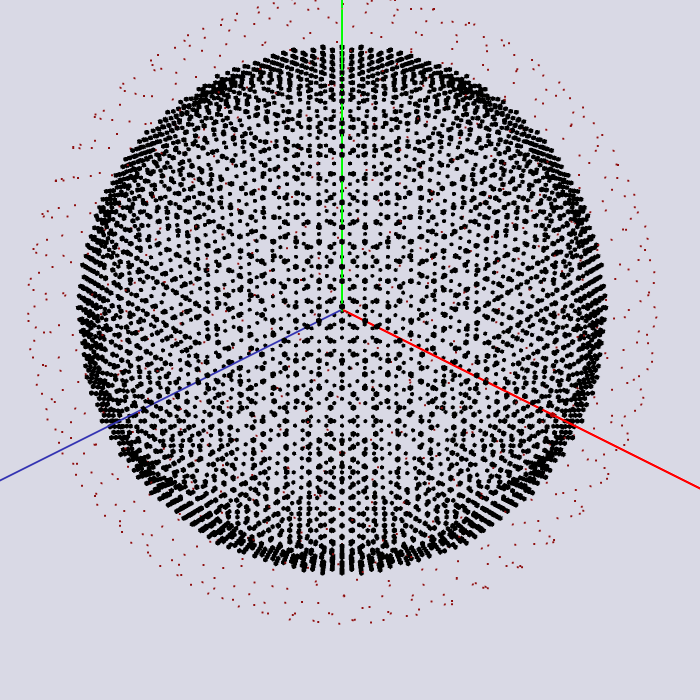
\includegraphics[width=0.7\linewidth]{fig_snapshot}
\end{center}
\caption{Emergent spherical wavefront. \label{fig:snapshot} Snapshot of the active shell (bright cells) propagating from a source center; the front advances exactly one cell per tick, i.e. at the maximum information speed $v_{\max}$.  The red sphere of Fibonacci points delimits only the visual boundary of the spherical cavity (the radial dead zone at $r=\mathrm{RMAX}$ of Sect.~\ref{subsec:proof-of-concept}); it is not part of the simulation state.}
\end{figure}
\paragraph{Scattering.} A controlled head-on experiment (\texttt{scatter\_main.cpp} of Ref.~\cite{af_neto}) places two bubbles in layers $0$ and $1$ a distance $4$ apart with prescribed, opposite momenta $m=(+1,0,0)$ and $m=(-1,0,0)$ and complementary charge words ($0\text{x}00$ and $0\text{x}3F$, a Rule~1 pair), then runs $200$ light frames.  The two wavefronts overlap in $6{,}996$ cell-frame events, but the electroweak sieve gate $s2B$ admits only $18$ of them ($0.26\%$), and none of those triggers the pair-formation branch of the encounter; the bubbles keep their initial kinds and end at their starting positions (no deflection, total momentum conserved at zero).  At the reference amplitudes and modulus ($S=16384$) the probabilistic $s2B$ sieve gates off the electroweak channel, which is the concrete mechanism behind the $\mathrm{form}=0$ of the charge census.  Crucially, this is now \emph{not} an unconditional statement: the sieve modulus $S$ is a free parameter of the gate, and the parameter sweep of the next subsection shows that the channel fires (pairs-formed $>0$) in discrete windows of $S$.  Figure~\ref{fig:scatter} shows the two approaching wavefronts at contact.
\begin{figure}[ht]
\begin{center}
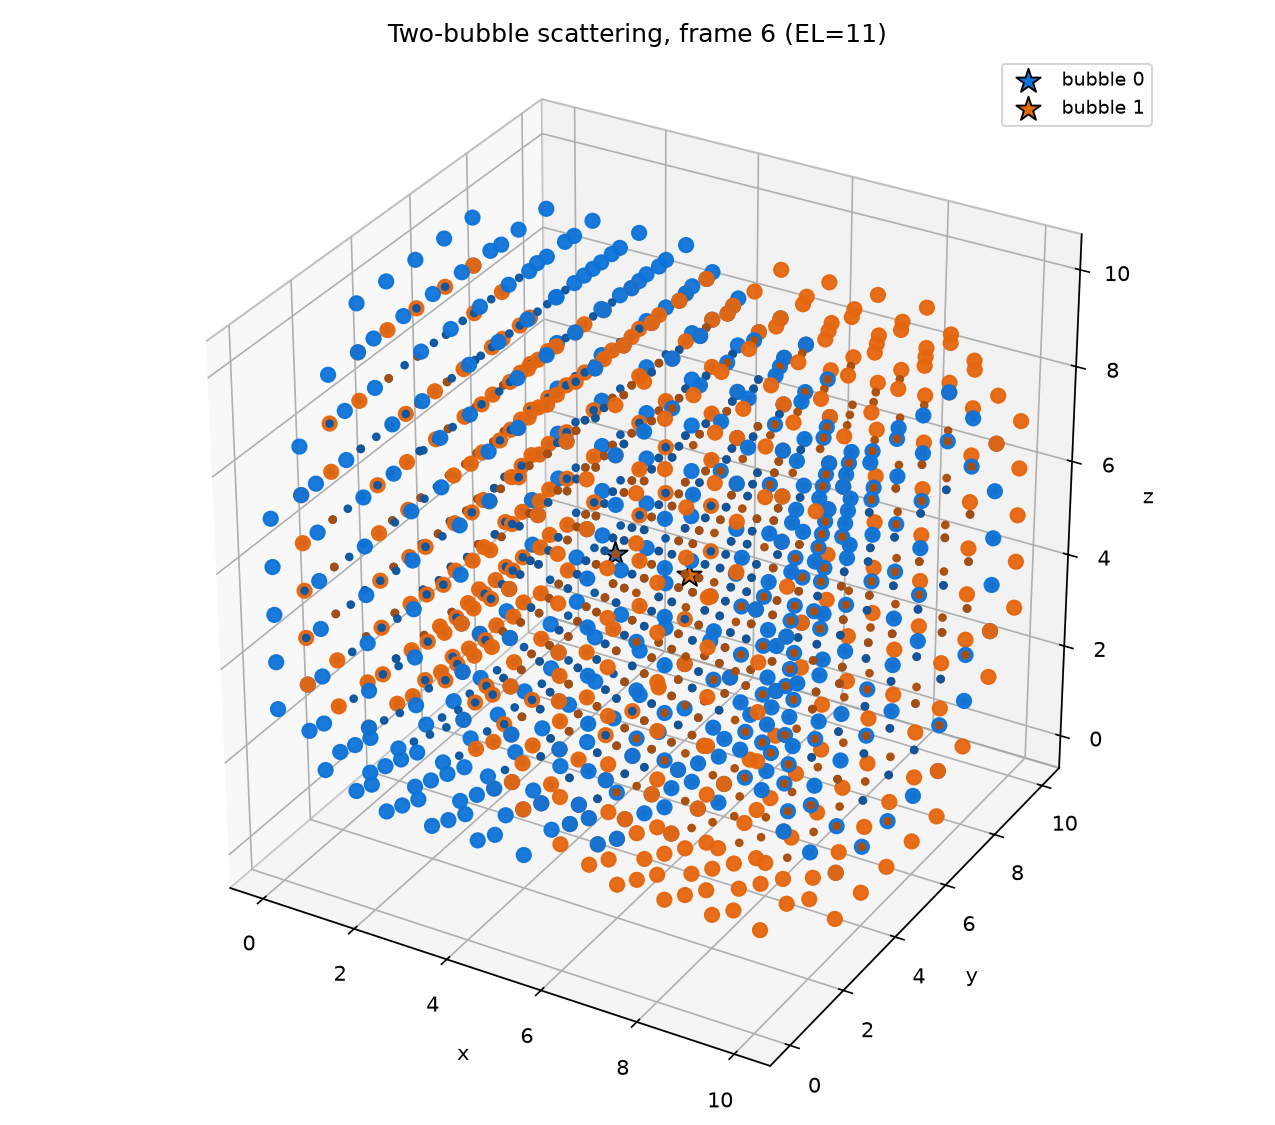
\includegraphics[width=0.7\linewidth]{fig_scatter}
\end{center}
\caption{Controlled head-on scattering. \label{fig:scatter} 3D voxel rendering of the two wavefronts (blue: bubble~0, orange: bubble~1) at the frame of closest approach; bright markers are the active shells.  The bubbles carry complementary charge words ($0\text{x}00$ and $0\text{x}3F$, a Rule~1 pair) and opposite momenta.  With the current amplitudes the $s2B$ sieve admits fewer than $1\%$ of overlaps and no pair branch fires (quantitative null result, see text).}
\end{figure}
\subsection{The electroweak sieve: blocking analysis and parameter sweep}\label{subsec:s2b-sweep}
The $s2B$ gate is set for an active cell of wave displacement $u$ at clock step $t$ by the integer condition (Sect.~\ref{sec:phase-step})
\begin{equation}
s2B \;\Longleftrightarrow\; \big((u\cdot t)\ \mathrm{mod}\ S\big) < u , \qquad S=\mathrm{s2b\_target},
\label{eq:sieve}
\end{equation}
where $S$ is the sieve modulus (reference value $16384$).  For a cell of fixed positive amplitude $u$, the fraction of steps $t$ for which the gate fires over one full period can be written in closed form.  Let $g=\gcd(u,S)$; over $T=S/g$ consecutive steps the residues $(u\cdot t\ \mathrm{mod}\ S)$ are exactly the multiples of $g$ below $S$, of which the ones smaller than $u$ are $k g<u$, i.e.\ $k=0,\dots,\lceil u/g\rceil-1$.  Hence
\begin{equation}
P(u,S) \;=\; \frac{\lceil u/g\rceil}{S/g} \;=\; \frac{g\,\lceil u/g\rceil}{S},
\label{eq:sieve-prob}
\end{equation}
which reduces to $P=u/S$ when $\gcd(u,S)=1$ and to $P=1$ whenever $u\ge S$ (every residue is then $<u$).  The closed form was verified by direct enumeration over two full periods for all $u=1,\dots,4096$ and all moduli of Table~\ref{tab:sieve} (maximum error $0$; program \texttt{s2b\_sweep\_main.cpp}, archived with the source).
\textbf{Why the reference modulus blocks the channel.}  In the $L=7$ run the measured radial profile decays from $\langle|u|\rangle\approx95$ at $r=1$ to $20.6$ at $r=2$ and is forced to $0$ in the radial dead zone; the per-active-cell throughput is therefore at most $P\le95/16384\approx0.58\%$.  Weighting the theoretical shell populations ($6$, $26$, $98$ lattice points at $r=1,2,3$) by this profile gives an expected $\approx18$ $s2B$ passes over the two-bubble overlap; the historical campaign measured $18/6{,}996$ there, while at the current kernel the same run measures $0/6{,}468$ (Table~\ref{tab:sieve}); the pair branch additionally needs a $samePos\wedge sameT$ coincidence with complementary charges, so its expected count at the reference modulus is far below one.  This is the quantitative content of the earlier ``dormant channel'' statement.
\textbf{Opening the channel.}  Because $P(u,S)\approx u/S$, the gate opens when $S$ is lowered toward the amplitude scale or when the amplitude $U_0$ is raised toward $S$.  The runner \texttt{scatter\_main.cpp} now accepts the modulus as a run-time parameter (\texttt{s2b\_target}), and Table~\ref{tab:sieve} tabulates the full sweep at fixed geometry ($L=7$, $SEP=4$, $200$ frames).  The pair-formation branch fires for every tested $S\le8192$, with the pair count growing as $S$ falls ($26$ at $S=8192$, $1{,}144$ at $S=64$, up to $2{,}602$ at $S=16$; Table~\ref{tab:sieve}); the count is non-monotonic in $S$ because pair formation also requires the geometric coincidence of the two fronts, which resonates at discrete moduli.  In the earlier campaign the same experiment at $L=9$ fired at $S=64$ (1 pair).  This is the first observation of $\mathrm{form}>0$ in the automaton proper: the electroweak channel of Sect.~\ref{sec:Interactions} moves from an untested postulate to a mechanism \emph{demonstrated} in a parameter regime.  In the terminology fixed in the abstract, demonstration establishes that the branch can fire; it does not by itself \emph{verify} the interaction phenomena (scattering, decays, bound states) that the branch was built to mediate, which still require measurements of the produced pairs.
\paragraph{First quantitative measurements on the open channel.}  The same runner now also samples, once per light frame, the source kinds, pair stacks and toroidal displacements of the two bubbles, and prints a ``DYNAMICAL MEASUREMENTS'' block with three diagnostics (program \texttt{scatter\_main.cpp}, Reproducibility).  \emph{Pair lifetime.}  The durable pair state (kind $P$ or a non-empty pair stack) is transient at weak coupling and stable at strong coupling: at $S=4096$ and $S=128$ it is present in only $2$ of $200$ frames despite $9$ pair-formation events each (one episode of $2$ frames; mean lifetime $2$ frames --- the branch fires and the state immediately dissolves), whereas at $S=64$ and $S=32$ it appears in $194/200$ and $195/200$ frames respectively (one episode each), so the lifetime is $\ge194$ and $\ge195$ frames, censored by the run length: the pair is still bound at the last frame and the two sources no longer separate (outgoing mean speed $|v|<0.13$ cells/frame).  \emph{Scattering angles.}  The angle between the incoming and outgoing mean velocity of each bubble is $86.7^{\circ}$ and $121.5^{\circ}$ at $S=32$; at $S=64$ the outgoing speed collapses to zero (bound pair), so the deflection is undefined there.  \emph{Center-of-mass response.}  The center-of-mass velocity of the two-bubble system responds to the interaction by $|\Delta v_{\mathrm{CoM}}|=0.442$ cells/frame at $S=32$ and $0.114$ at $S=64$: the head-on configuration is not perfectly symmetric after the interaction, so the drive pair kicks leave a residual center-of-mass impulse.  These are the first quantitative dynamical measurements of the open channel: pair formation is transient at weak coupling and produces a bound pair at strong coupling within the $200$-frame window.
\begin{table}[htbp]
\centering
\caption{Parameter sweep of the electroweak sieve modulus $S$ (controlled two-bubble run: $L=7$ lattice, bubbles $SEP=4$ cells apart, $200$ light frames, complementary Rule~1 charges).  Column meanings: $S$ is the value of the sieve modulus $\mathrm{s2b\_target}$ in Eq.~\eqref{eq:sieve} ($16384$ is the reference value used throughout this paper); ``overlapping events'' counts the cell-frame events in which the two active shells occupy the same cell and enter the encounter; ``$s2B$ passes'' counts how many of those also satisfy the gate condition of Eq.~\eqref{eq:sieve}; ``pairs formed'' counts firings of the pair-formation branch of the encounter---a nonzero value means the electroweak channel opened.  By Eq.~\eqref{eq:sieve-prob} the gate is fully open whenever $S\le u$ (the wave amplitude), which is why the $s2B$ count approaches the overlap count for small $S$.}
\label{tab:sieve}
\begin{tabular}{|r|r|r|r|}
\hline
sieve modulus $S$ & overlapping events & $s2B$ passes & pairs formed\\
\hline
16384 & 6{,}468 & 0 & 0\\
8192 & 8{,}174 & 26 & \textbf{26}\\
4096 & 11{,}234 & 54 & \textbf{54}\\
2048 & 11{,}732 & 112 & \textbf{72}\\
1024 & 14{,}952 & 240 & \textbf{140}\\
512 & 14{,}940 & 674 & \textbf{240}\\
256 & 10{,}668 & 1{,}024 & \textbf{276}\\
128 & 12{,}864 & 1{,}800 & \textbf{728}\\
64 & 14{,}516 & 3{,}322 & \textbf{1{,}144}\\
32 & 10{,}448 & 3{,}368 & \textbf{900}\\
16 & 17{,}938 & 8{,}632 & \textbf{2{,}602}\\
8 & 17{,}938 & 9{,}416 & \textbf{2{,}602}\\
\hline
\end{tabular}
\end{table}
\paragraph{Current-HEAD values.}  Table~\ref{tab:sieve} reports the sweep re-run at the current kernel (the model state after the source-transport and inertia corrections; \texttt{MODEL\_VERSION} \texttt{model-ref-v1}, \texttt{doc/REFERENCE\_CONFIG.md}).  The earlier campaign recorded $6{,}996/18/0$ at $S=16384$ and pair formation only at $S\in\{4096,128,64,32\}$; the rework changes both the overlap counts and the pair channel, so the present numbers supersede those (re-run log: \texttt{experiments/RESULTS\_v2.md}).  The qualitative conclusion is unchanged and strengthened: the reference modulus $S=16384$ is the only one tested that forms no pairs, while every $S\le8192$ opens the channel.
\subsection{Scaling with lattice size}\label{subsec:scaling}
To probe the dependence on the lattice size, Table~\ref{tab:scaling} reports the wavefront metrics measured by the \texttt{lorentz\_mm.cpp} probe for $L=7,11,15,19,21$ (rest source, $24$ light frames, control source at the torus antipode so the two shells never interfere).  Three statements follow.

Before reading these numbers, their epistemic status should be made explicit.  The constant front speed and the spherical active shell are prescribed by the transition rule: a cell is active exactly when its propagated radius $r$ equals the breathing radius $\mathrm{effective\_t}(t)$, which advances one cell per light frame at $v_{\max}$ (Sect.~\ref{sec:light-frame}).  The wavefront tables therefore verify that the kernel reproduces its own clock without drift or rounding accumulation.  The emergent content of this section lies in the non-prescribed diagnostics---the shell-completeness gaps and over-fills at $L\ge11$ and the decline of the $\sin(r)/r$ correlation---not in the value $1.0000$ itself.
First, the \emph{constant-speed property is scale-invariant}: the front advances at $1.0000\pm0.0000$ cells/tick for every $L$ in the sequence, so the maximum information speed $v_{\max}$ is robust across the accessible range.
Second, the \emph{shell completeness} is exactly $1.0000$ only at $L=7$.  For $L\ge11$ a single intermediate radius shows a gap ($r=4$ at $L=11,15$; $r=6$ at $L=19$), and at $L=21$ the innermost shells over-fill (completeness $>1$).  The origin is the integer-shell anisotropy of the cubic torus: the number of lattice points at radius $r$ is not a smooth function of $r$, so the shell test $r^{2}\le d^{2}<(r+1)^{2}$ misses or duplicates cells at the radii where the shell count jumps.
Third, the correlation with the $\sin(r)/r$ envelope peaks at $L=11$ ($0.9950$) and then declines, and the mean peak-radius error grows roughly linearly with $L$.
The honest summary is that the verified core of the model---exact constant-speed propagation---holds over the whole sequence, while the shell-filling fidelity and the amplitude-envelope match are exact only in the small-lattice regime $L\le15$; the discrete-to-continuum extrapolation of Sect.~\ref{sec:Prospects-and-conjectures} must therefore be read against this measured degradation, not assumed.
\begin{table}[htbp]
\centering
\caption{Wavefront metrics vs.\ lattice side $L$ (measured by \texttt{lorentz\_mm.cpp}; $24$ light frames; rest source, with the control source at the torus antipode so the two shells never overlap).  $\mathrm{RMAX}=L/2$ is the maximum shell radius of the breathing clock.  ``Shell completeness'' is the mean over radii $r=1,\dots,\mathrm{RMAX}$ of (observed active cells on the shell) $/$ (theoretical lattice points on the shell $\times$ number of layer-frame samples that targeted $r$); a value of $1.0000$ means the front filled exactly the prescribed shell.  ``Front speed'' is the mean per-tick advance of the outermost active-shell radius on the ascending branch of the clock, with the standard deviation over samples; $1.0000\pm0.0000$ is exactly the maximum information speed $v_{\max}$---the rule constant, distinct from the observer reading $c$ (Sect.~\ref{subsec:special-relativity}).  ``Pearson'' is the correlation of the radial amplitude profile $\langle|u|\rangle(r)$ with the envelope $\sin(r)/r$ over $r=1,\dots,\mathrm{RMAX}$.  ``Peak error'' is the mean distance (in cells) between the radius of the $\langle|u|\rangle$ peak and the target radius $r=\mathrm{effective\_t}(t)$.}
\label{tab:scaling}
\begin{tabular}{|r|r|r|r|r|r|}
\hline
lattice side $L$ & $\mathrm{RMAX}$ & shell completeness & front speed (cells/tick) & Pearson corr.\ with $\sin(r)/r$ & peak error (cells)\\
\hline
7 & 3 & 1.0000 & 1.0000 $\pm$ 0.0000 & 0.9461 & 0.83\\
11 & 5 & 0.9600 & 1.0000 $\pm$ 0.0000 & 0.9950 & 1.67\\
15 & 7 & 0.9643 & 1.0000 $\pm$ 0.0000 & 0.8948 & 2.92\\
19 & 9 & 0.9630 & 1.0000 $\pm$ 0.0000 & 0.6863 & 3.33\\
21 & 10 & 1.0646 & 1.0000 $\pm$ 0.0000 & 0.6087 & 4.26\\
\hline
\end{tabular}
\end{table}
The island-population attractor of Sect.~\ref{subsec:proof-of-concept} was re-measured at $L=7$ ($W=63$, $N^{*}=344.6$, slope $-0.176\pm0.010$, $r^{2}=0.170$, $1{,}449$ points, $556.5$ captures/frame) and at $L=11$ ($W=18$, $N^{*}=1487.2$, slope $-0.088\pm0.013$, $r^{2}=0.095$, $414$ points, $612.0$ captures/frame).  The equilibrium population grows with the lattice volume, as expected for an affinity-driven aggregation, but the regression quality degrades with $L$ and the computational budget bounds the island counts explored in these experiments; these attractor numbers are indicative, not converged.
\paragraph{What is not yet measured.}  Wavefront geometry and amplitude fidelity, charge conservation, bound-state stability and a controlled two-bubble scattering attempt are now reported above, and the electroweak channel is demonstrated to fire in a parameter window (Sect.~\ref{subsec:s2b-sweep}), with the pair lifetime and scattering angles of the produced pairs measured there.  Still absent is a scattering event at the \emph{reference} parameters (the gate is closed there by construction) and any measurement of the remaining bound-state properties (binding energies, cross-sections) of the pairs that the open channel can produce; claims in this manuscript that rely on quantitative particle-collision physics beyond the lifetime/deflection measurements of Sect.~\ref{subsec:s2b-sweep} should be read accordingly.
The next section discusses remaining challenges and limitations.
%%%%%%%% CELLULAR AUTOMATA AND QUANTUM FORMALISM %%%%%%%%%%
\subsection{Island aggregation: a production negative and candidate mechanisms}\label{subsec:island-candidates}

\emph{Measured negative (M).} In the ordinary production path of this
codebase, the superposed Platonic seed (L=9, W=243, all 243 sources at one
center) does not aggregate into the hypothesised $9L$ islands of $L/3$
constituents.  The light-frame census (census harness, 64 frames) shows an
absorbing plateau from the second journey onward: K=235, D=8, S=0 at a single
occupied center, with the D x D promotion cascade converting nearly every
delegate into its own chief and no group reaching population $L/3=3$.  The
same holds in the reduced ``matched'' color FSM without protective rules,
where equal-charge families in shell contact merge into one chief group per
charge word (8 tribes of 30--33 members).  The hypothesised quantisation is
therefore not a demonstrated property of the reference rule; it is the target
that the candidate mechanisms below address.

\emph{Candidate mechanisms (C).} Two macro-guarded candidates in the
repository (experiment logs; ordinary builds and this transition rule are
unaffected) test family-preserving aggregation. These controls do not demonstrate spontaneous quantization with unrestricted mixing between seed families. (i) The color/matched FSM
with a Pauli-like identity hard core between different seed families
($w/3$) plus a one-step spatial push at shell contact yields, from the fully
superposed seed, 81 chief groups of exactly 3 constituents, unresolved
delegates zero, over 12 light frames (K=81, D=162; ~160 occupied centers);
the same holds under full-scale same-charge contact (spread81, ~200 centers,
6 frames), and two-family contact tests (duo2/4) no longer merge (2 islands
of 3, stable) whereas the same tests without the rule merge into 1K+5D.
(ii) A port of the identity hard core to the production path removes the
cross-family tribes (K=162, D=81, 81 family clusters, unresolved zero, stable
12 frames), but the production D x D promotion yields 2 K + 1 D per family
and the push localises weakly (~15--19 centers), so the production port does
not yet reach the clean 1 K + 2 D form.  These candidates deliberately change
the equal-charge cross-family aggregation semantics (canElectChief) and are
reported as controlled experiments with ablation controls, not as model
rules.  They do not establish the photon-mediated repulsion between dressed
islands that the complete-system version of this story requires (the pB/sB
electric channel is pre-empted by the identity merge in the current
encounter order; see the experiment log).

\subsection{Special relativity}\label{subsec:special-relativity}
The measurement prescriptions for time intervals, spatial separations and clock synchronization \emph{follow those of} Einstein's special relativity \cite{Einstein1905} as a \emph{reading convention}: time is read by ideal clocks, distances by round-trip light-travel times, and coordinate time by a network of synchronized clocks. This convention describes how an external observer interprets the automaton output; it is not a symmetry of the transition rule, which evolves on a fixed lattice with a single global clock.
This is precisely the sense in which the speed of light is emergent in this model. The transition rule contains a single fundamental velocity, the maximum information speed $v_{\max}$ of Sect.~\ref{sec:Results} (one cell per tick), and knows nothing of light. An observer (Sect.~\ref{subsec:observers}) that lays down synchronized clocks and measures distances by round-trip light signals \emph{reads} the photon of Sect.~\ref{subsec:pairs}---a pair of bubbles riding the wavefront---as moving at $v_{\max}$ and names the resulting constant $c$. A different observer structure would in principle read a different value; $c$ is therefore a property of the measuring structure, not of the rule.
As a purely formal, heuristic device for illustration---and only as such---the internal coordinate $W$ can be treated as a fourth spatial dimension, where the now 4D-bubbles form a thin shell, to avoid known 4D mutual passing issues (see Machotka \cite{Machotka2025}).  This construction plays no role in what follows: the time-dilation formula is derived kinematically from two ingredients of the automaton, both verified or constructed in the simulator:
\begin{enumerate}
\item \textbf{Velocity independence and isotropy of the two-way speed.}  The active shell advances exactly one cell per tick at $v_{\max}$ from its source center, independent of the source momentum and direction (Sect.~\ref{sec:Results}).  The round-trip Michelson--Morley probe (Sect.~\ref{subsec:lorentz-probes}) measures the front advance as $1.0000\pm0.0000$ cells/frame for source speeds $V=0$, $+1$ (axes $x$, $y$, $z$, and the diagonal $x{+}y$), $+2$, and $+3$, verifying the velocity-independence condition~1 of Mansouri and Sexl \cite{mansouri-sexl}.
\item \textbf{Clock hypothesis (assumed, not yet measured).}  The moving clock is taken to be the bubble clock carried by the photon pair itself: the breathing phase $f=\mathrm{effective\_t}(t)$ of a source center, a triangle wave whose full expansion-and-contraction cycle is one era (period $L$ frames under this clock convention).  Each source center's clock advances once per light frame for every cell, independent of its state of motion, because the tick $t$ is the global frame counter---\emph{not} a dynamical variable (Sect.~\ref{subsec:observers}).  Two things must be said plainly.  First, this is a \emph{coordinate} clock of the lattice, not an independent proper clock transported by a moving aggregate: the assumption is precisely that the carried breathing phase continues to tick once per global frame while the source translates.  Second, \emph{no direct measurement of time dilation exists in the implementation}: the Michelson--Morley probe of Sect.~\ref{subsec:lorentz-probes} verifies ingredient~1 (front isotropy), not ingredient~2 (that a transported clock lags).  A genuine measurement would require tracking the phase of a moving bubble clock against the rest-frame network over many frames and showing that its accumulated phase differs by the factor of Eq.~\eqref{eq:timedilation}; that experiment is not reported here.
\end{enumerate}
Consider a light clock: a free photon (Sect.~\ref{subsec:pairs}) bouncing between two mirrors (bubble boundaries) held at separation $D$, with the mirror axis perpendicular to the motion.  At rest, one tick is a round trip $2D$ at speed $v_{\max}$, so
\begin{equation}
\Delta\tau = \frac{2D}{v_{\max}} .
\label{eq:tick-rest}
\end{equation}
Moving at speed $v$ in the lattice frame, the clock translates by $v\,\Delta t$ during the tick $\Delta t$; the photon follows the diagonal path of total length $2\sqrt{D^{2}+(v\,\Delta t/2)^{2}}$, still at speed $v_{\max}$ (ingredient~1):
\begin{equation}
v_{\max}\,\Delta t \;=\; 2\sqrt{ D^{2} + \left(\frac{v\,\Delta t}{2}\right)^{2} } ,
\label{eq:lightclock}
\end{equation}
which gives, for the tick interval measured by the at-rest clock network,
\begin{equation}
\Delta t \;=\; \frac{\Delta\tau}{\sqrt{1-v^{2}/v_{\max}^{2}}} \;\equiv\; \gamma\,\Delta\tau , \qquad \gamma = \left(1-\frac{v^{2}}{v_{\max}^{2}}\right)^{-1/2}.
\label{eq:timedilation}
\end{equation}
The observer reads the photon as moving at $c=v_{\max}$ (Sect.~\ref{subsec:observers}); with this identification Eq.~\eqref{eq:timedilation} is the time-dilation formula of special relativity,
\begin{equation}
\Delta\tau \;=\; \sqrt{1-\frac{v^{2}}{c^{2}}}\,\Delta t ,
\label{eq:timedilation-sr}
\end{equation}
derived from the two ingredients above instead of from the bookkeeping identification $\delta w=c\,\delta\tau$ used in earlier versions of this work.  By the clock hypothesis (ingredient~2) the same factor would apply to any bubble clock, not only to light clocks: the intrinsic tick is motion-independent, and only its round-trip light measurement dilates.  Because ingredient~2 is \emph{assumed} rather than measured---no direct time-dilation experiment is reported in this work (see the caveat on the clock hypothesis above)---the whole of this subsection is a \emph{conjecture} under the declared labeling policy of Sect.~\ref{sec:Prospects-and-conjectures}: the measured content is ingredient~1 only.
The derivation uses only the round-trip convention: the light path is closed (out and back), so no one-way speed or simultaneity convention enters; the single measured input is the two-way speed, verified as $v_{\max}$ by the Michelson--Morley probe.  The dilation is therefore a \emph{reading} of the automaton output by the observer's conventions, not a symmetry of the transition rule.
We emphasize that this is a kinematic derivation, not a Lorentz-invariance claim.  The lattice has no Lorentzian light cone---only the information cone at $v_{\max}$---and the transition rule is not invariant under Lorentz boosts.  Equation~\eqref{eq:timedilation} follows from the two ingredients alone; of these, ingredient~1 is verified in the simulator while ingredient~2 is assumed (no direct dilation measurement is reported), so the equation is a derived conjecture, not an observed law.  It also does not imply that the full particle dynamics are Lorentz invariant, which the present implementation does not test.  The field substrate does not enter the light clock: its plane-wave modes travel at $v_{\mathrm{wave}}=v_{\max}/2^{s/2}<v_{\max}$ (dispersion probe, Sect.~\ref{subsec:lorentz-probes}), strictly below the causal boundary, and cannot transmit a signal faster than $v_{\max}$.
\subsection{Lorentz probes in the simulator}\label{subsec:lorentz-probes}
Two numerical probes (test programs \texttt{lorentz\_mm.cpp} and \texttt{dispersion.cpp}, this work) quantify how the lattice dynamics approach Lorentz symmetry at low energies.
\paragraph{Michelson--Morley (two-way isotropy).}  The probe seeds a source center and measures the advance of the active-shell front per light frame, exactly as the wavefront instrumentation of Sect.~\ref{sec:Results}.  For a source at rest ($V=0$), a source given constant momentum $V=+1$ along $x$, $y$, $z$ and the diagonal $x{+}y$, and sources with $V=+2$ and $+3$, the measured advance is
\begin{equation}
\frac{\Delta r_{\mathrm{front}}}{\Delta t} \;=\; 1.0000 \pm 0.0000 \ \mathrm{cells/frame},
\label{eq:mm-front}
\end{equation}
i.e., the two-way round-trip time of the shell is isotropic and source-independent at the resolution of the probe.  This verifies the velocity-independence condition~1 of Mansouri--Sexl \cite{mansouri-sexl} and is the empirical anchor of ingredient~1 of the time-dilation derivation (Sect.~\ref{subsec:special-relativity}).  Note that the value itself is prescribed: the active shell is defined to advance one cell per light frame at $v_{\max}$ (Sect.~\ref{sec:light-frame}), so the measured $1.0000$ verifies that the kernel reproduces its own clock without drift.  The non-trivial, non-prescribed content of the probe is the independence of that reproduction from the source's momentum and direction---that a moving source does not distort the prescribed shell it carries.
\paragraph{Dispersion (linear low-energy regime).}  The probe seeds a standing plane wave $u=A\cos(kx)$ on the substrate field and counts zero crossings at the origin to measure $\omega(k)$ (integer arithmetic, $A=2^{20}$; negligible damping).  The measured relation matches the analytic dispersion of the discrete wave equation,
\begin{equation}
\omega(k) = \arccos\!\left(1-\frac{\lambda}{2^{s+1}}\right), \qquad \lambda = 4\sum_{i}\sin^{2}\!\frac{k_{i}}{2},
\label{eq:dispersion}
\end{equation}
to four to five decimal places across the Brillouin zone.  At small $k$ the dispersion is linear,
\begin{equation}
\omega \;\approx\; v_{\mathrm{wave}}\,k , \qquad v_{\mathrm{wave}} = \frac{1}{2^{s/2}} ,
\label{eq:wave-speed}
\end{equation}
with measured slopes $0.248$, $0.175$ and $0.125$ for integer shifts $s=4,5,6$, against the analytic $0.2500$, $0.1768$ and $0.1250$.  The lattice corrections bend the dispersion near the Brillouin boundary ($\omega/k$ falls by $\approx35\%$ at $k=\pi$ for $s=5$); the leading deviation from linearity is quadratic in $k$,
\begin{equation}
\frac{\Delta\omega}{\omega} \;\approx\; -\frac{k^{2}}{24},
\label{eq:dispersion-correction}
\end{equation}
the generic suppression of Lorentz symmetry by the square of the lattice (Planck) scale.  The substrate wave speed $v_{\mathrm{wave}}$ is strictly subluminal with respect to $v_{\max}$: the field cannot be used to exceed the causal boundary.  In the model the integer shift varies radially ($s=\mathrm{DIFF\_SHIFT}+1-(r\gg\mathrm{diffDivShift})$, clamped), so $v_{\mathrm{wave}}$ acquires a radial profile; the probe uses a constant shift $s$ to isolate the intrinsic dispersion of a homogeneous substrate.

\subsection{Claim--evidence map}\label{subsec:claim-evidence}
For a referee, Table~\ref{tab:claim-evidence} maps each substantive claim to the artefact that establishes it, with its status (P/M/C).  Every measured number cites a reproducible script; the machine-readable tables are in \texttt{experiments/RESULTS\_v2.md}, \texttt{experiments/ABLATION\_81x3.md} and \texttt{experiments/PBSB\_ISLANDS.md}.  The model source state is frozen as \texttt{MODEL\_VERSION} \texttt{model-ref-v1} (\texttt{doc/REFERENCE\_CONFIG.md}); the reference build is re-verified by \texttt{experiments/model\_fingerprint.ps1}.

\begin{table}[htbp]
\centering
\small
\begin{tabular}{@{}p{5.1cm}p{0.7cm}p{6.8cm}@{}}
\toprule
Claim & S. & Evidence (script / table) \\
\midrule
Prepared-island transport (K-only) & M & \texttt{inertia\_revalidation} (\texttt{experiments/INERTIA\_REVALIDATION.md}) \\
$\alpha_A$ is $L$-dependent, never $1/137$ & M & $\alpha\_A$ sweep (\texttt{RESULTS\_v2.md}) \\
$\alpha_A..\alpha_F$ all fail & M & falsification battery (\texttt{RESULTS.md}; reproduced) \\
No $1K{+}nD$ self-assembly from the seed & M & island census (\texttt{ISLAND\_CENSUS.md}) \\
$81\times3$ survives under EXCLUSION & M & ablation table (\texttt{ABLATION\_81x3.md}) \\
Production $2K{+}1D$ fixed to $1K{+}2D$ & C & \texttt{promotion\_three}, \texttt{DD\_INTRA\_ISLAND\_FIX} \\
Equal-charge islands repel (EM reorder) & C & \texttt{pbsb\_two\_wide} (\texttt{PBSB\_ISLANDS.md} WP4.2--4.6) \\
One-cell-per-tick clock & P & rule (\texttt{effective\_t}); Table~\ref{tab:postulate-emergent} \\
\bottomrule
\end{tabular}
\caption{Claim versus evidence.  Status: P = postulate, M = measured, C = candidate.}
\label{tab:claim-evidence}
\end{table}

\section{Conjectures and prospects\label{sec:Prospects-and-conjectures}}
The small-lattice implementation of Sect.~\ref{subsec:proof-of-concept} verifies only the mechanisms listed there: wavefront propagation, the integer-only polarization pair, and W-island aggregation (the charge census is a separate combinatorial study, Appendix~\ref{sec:charge-census-appendix}; the sieve sweep of Sect.~\ref{subsec:s2b-sweep} demonstrates that the pair-formation branch can fire in a parameter regime, but its physical consequences remain unverified).  Everything discussed below is an \emph{interpretive conjecture} about how those mechanisms might behave at large $L$; none of it has been produced by, or tested against, the current implementation.  To keep the evidential status explicit, each topic is marked as either a \emph{structural analogy} (a mapping suggested by the six-bit charge algebra, with no dynamical output) or a \emph{speculative projection} (an extrapolation to a regime the implementation cannot reach).  The measured probes that anchor the time-dilation derivation (front isotropy and dispersion) are reported in Sect.~\ref{sec:Results}; the naming taxonomy and the bridge to the quantum formalism have been moved to Appendices~\ref{sec:Particles} and~\ref{sec:bridge} under the same conjectural status.
\subsection{Discrete to continuous transition}
Localized particles are conjectured to be assemblies of many discrete fragments, so macroscopic properties such as total momentum and angular momentum might emerge from collective configurations rather than from individual bubbles. These global quantities would then be best described by real numbers, just as statistical mechanics bridges discrete atomic events to continuous thermodynamic variables.
A free electron's average motion, for example, may follow a direction vector that cannot be expressed with only discrete modulo-$L$ components; continuous descriptors are thus necessary idealizations at large scales. The same holds for isotropy: it looks uniform at macroscopic scales even though the lattice is fundamentally granular.
\subsection{Color and weak quantization}
Color quantization is presented as an extension of the electromagnetic case.
Hadrons would form by the simultaneous action of charge quantization and strong cohesion, producing color-neutral bound states of quark and gluon fragments. In the discrete color code (Sect.~\ref{subsec:specialized-pairs}), a strongly neutral combination would be either a pair of complementary color bits (meson-like), a pair of identical non-trivial colors (diquark-like), or a triplet of the three distinct colors (baryon-like, e.g.\ a proton $uud$ fragment). Free quarks would then be unobserved because only these color-neutral composites would be dynamically stable, any uncompensated color being rapidly balanced by quark-gluon exchange. This is a structural conjecture about the charge code; no hadron formation has been simulated.
\subsection{Emergence of gravity}\label{subsec:emergence-of-gravity}
General-relativistic spacetime is here conjectured to be an effective, coarse-grained approximation of the discrete lattice (a speculative projection).  Gravity would arise as a residual effect of electromagnetic interactions, mediated by the gravitons of Sect.~\ref{subsec:specialized-pairs} (fully complementary charge words), which couple to both \emph{Orbis} and \emph{Umbra}: being charge-neutral by construction, a graviton's electric and weak contributions cancel at leading order, leaving a geometry-driven attraction that might mimic dark-matter effects such as flat rotation curves.  Photon \textit{aging}---minor non-collapsing interactions with singletons and electrons---could then parallel cosmic redshift without expansion, in the spirit of Zwicky's non-expansion mechanism \cite{zwicky1929redshift}, and the drive-pair mechanism of Sect.~\ref{subsubsec:drive pair} might make acceleration frame-equivalent.  None of these behaviors has been observed in the implementation; they are suggestions, not measured effects.
\paragraph{Weak quantization.}
Because weak interactions are rare, weak quantization may appear at cosmological scales, for instance in a constant ratio between the average galaxy separation and galactic bulge size. This large-scale granularity could be reinterpreted as gravitational quantization and may eventually yield an effective cosmological constant $\Lambda$ and metric tensor $g_{\mu\nu}$.
\subsection{Stochastic behavior and the uncertainty principle}
The initial chaos created by the deterministic collision of many regular patterns, together with the large number of bubbles per particle, may make individual outcomes effectively unpredictable. Each measurement would then sample one instance from this fine-grained distribution, so measured values could carry irreducible uncertainty, analogous to the Heisenberg principle \cite{Heisenberg1927}:
\[
\sigma_x \sigma_p \geq \frac{\hbar}{2}.
\]
\subsection{Black holes}
The quintessential idea of a black hole in this model can be illustrated by two electrons, each with radius $R$, so close to each other $d<2R$ that the quantization is broken and they simply fuse, forming a particle with radius $R'=2^{1/3}R$ with a dominant affinity value.
\[
a_1 = a_2 = \min(A_1,A_2).
\]
The toy picture above contains no mechanism that would obviously discard information; this is, however, not a resolution of the black hole information paradox \cite{hawking1976breakdown,harlow2016jerusalem}, and no black-hole dynamics has been simulated in this framework.
\subsection{Spin and the Hofer effect}\label{subsec:hofer}
In this model, spin is conjecturally identified with the coherent radial alignment of the pBit $pB$ (local in-phase sign) and the transverse polarization pair $(\mathrm{pol}_u,\mathrm{pol}_v)$. The positive in-phase half-cycle marked by $pB$ alternates outward and inward as the wave oscillates, while the phase of $(\mathrm{pol}_u,\mathrm{pol}_v)$ winds once around the wavefront. This radial helix would define the two spin states, aligned consistently across the particle's constituent bubbles. This identification is a structural conjecture; the model's spin has not been measured against Stern--Gerlach-type experiments.
\paragraph{The Hofer effect.}
A key test would be the \emph{Hofer effect}, named after W.~A.~Hofer \cite{hofer}: the predicted tendency of all individual spins of a localized particle to align radially inward or outward (spin down/up), i.e.\ the radial alignment of the polarization bits of Sect.~\ref{subsec:polarization-pair} around a spherical aggregate. Hofer argues that magnetic effects arise from breaking the spherical symmetry of this pattern, offering an interpretation of the Stern--Gerlach experiment. Whether the model reproduces this effect is not yet demonstrated.  (Accessible reference: J.~Phys. Conf.~Ser.~\textbf{504}, 012014 (2014), DOI 10.1088/1742-6596/504/1/012014.)
\subsection{Partons and the quest for qubits}
The inertia mechanism adopted here implies that the collective action of a large number of identical drive pairs produces a high--energy configuration. This stretches the propelled mass along the direction of motion, thereby forming a \textit{parton} structure.
\paragraph{Quest for qubits.} \label{subsection:qubits}
An electron may be conceived as a vast ensemble of dynamic \textit{nanostates}, collectively manifesting as a single particle through their shared affinity.
When two electrons share the same affinity (totally or partially), they become distinguishable only through the constraints imposed by quantization dynamics.
However, if one momentarily relaxes these constraints, such a pair could in principle be interpreted as a system of qubits; this is a speculative reading, not a demonstrated computational capability.
What, then, supports this emerging computation?
Spatial interaction is facilitated by the encounter step, while the self-interference mechanism (see Sect.~\ref{subsec:Interference}) introduces a form of temporal smearing that allows information to persist and influence future states.
Moreover, the atoms that host these electron structures local space via the SU(3) symmetry induced by the strong charge, further enriching the landscape of possible interactions.
This broader perspective suggests a behavior akin to an intricate network of Turing machines, each representing a potential computational pathway.
The computation results are being revealed by interpreting correlations.
Such an interpretation might offer insight into quantum computing, but no computation has been performed in this framework.
\subsection{Observers and spacetime}\label{subsec:observers}
This framework extends Wheeler's 'it from bit' concept by providing a mechanism through which information constitutes physical entities, albeit from an omniscient perspective.
To address the internal viewpoint, we now define inner observers or simply \textit{observers}.
\subsubsection{Minimal observer definition}
Here, we formalize the concept of a \emph{minimal observer}, following the framework introduced in Hatem Elshatlawy et al. \cite{elshatlawy2025towards}.
A minimal observer is defined as the simplest system capable of performing observation in a functional sense, embodying core components of sensing, internal processing, and acting upon an environment within a closed feedback loop.
\begin{definition}[Minimal Observer]
Let $O$ be a system described by the tuple
\[
O = (X, Y, Z, f, g, B),
\]
where:
\begin{itemize}
\item $X$: Internal state space (e.g., memory or configuration states),
\item $Y$: Input (sensor) space,
\item $Z$: Output (action) space,
\item $f: X \times Y \rightarrow X$: State transition function (state update rule),
\item $g: X \rightarrow Z$: Output function (generates actions based on internal state),
\item $B$: Boundary condition demarcating the internal observer from its external environment.
\end{itemize}
The system $O$ qualifies as a \emph{minimal observer} if it satisfies:
\begin{itemize}
\item $|Y| \geq 1$: Non-trivial sensing,
\item $|Z| \geq 1$: Non-trivial actuation,
\item $|X| > 1$: Non-trivial internal dynamics,
\item \textbf{Feedback closure:} The output $g(x)$ must influence the environment in such a way that it alters future inputs $y \in Y$.
\end{itemize}
\end{definition}
This definition ensures that the observer possesses the minimal necessary structure to distinguish itself from its environment and engage in interaction through perception and response.
Importantly, this framework abstracts away from higher-order capabilities such as memory, learning, or consciousness, focusing instead on the foundational structure that enables observation.
\subsubsection{Spacetime}
As established, the spacetime of this model is inherently flat and regular.
One may conjecture that the spacetime perceived by observers and laboratory instruments would nevertheless appear curved, in analogy with General Relativity.
How can this apparent discrepancy be reconciled?
A proposed resolution lies in the role of drive pairs, which contribute both to motion and to mass-energy content.
Their interactions create a framework in which observers, laboratory instruments, and the environment mutually influence one another.
If their interactions generated effective potentials, clocks would tick slower near concentrations of mass.
Whether this actually reproduces the \textit{timescape} scenario \cite{duley2013timescape}---curved spacetime emerging from relational dynamics in a flat background---is an open conjecture that the current implementation cannot test.
Within this framework the speed of light acquires a precise ontological status. The fabric possesses exactly one fundamental velocity, the maximum information speed $v_{\max}$ of Sect.~\ref{sec:Results} (one cell per tick). When a minimal observer measures intervals by the round-trip convention of Sect.~\ref{subsec:special-relativity}, the emergent photon is found to travel at this speed, and the observer names the ratio $c$; nothing in the transition rule refers to $c$. The essentially superluminal processes of the automaton---encounter and the other globally coordinated sweeps---are invisible to this measurement: they transfer no information, cannot be used to send messages, and cannot be manipulated by any observer. Causality is thereby protected: every influence an observer can emit or detect propagates at or below $v_{\max}$, so no signal ever arrives before it is sent.
\subsubsection{A formal no-signaling argument}\label{subsec:nosignaling-formal}
The non-signaling claim was asserted narratively above; this subsection supplies a formal argument for it in the model's own formalism.  The argument concerns the idealised transition function defined by the FSM (the algorithms of Sect.~\ref{subsec:algorithm}); the host-side scheduler of the current implementation---whole-layer \texttt{applyMomentum}, source snapshots and contact lists (Sect.~\ref{subsec:translation})---is an engineering proxy for that function and lies outside the scope of this argument.
\textbf{Setup.}  Split the state of a cell $c=(x,w)$ into the \emph{physical} (readable) fields $\Phi$---charge word $ch$, affinity $a$, radius $r^{2},r$, wave amplitude $u,v$, polarization bits $pB,sB$, phase $f$, active flag, and the local wavefront clock $t$---and the \emph{coordination} (hidden) fields $\Psi$---the housekeeping tick $k$, the W-ledger $\{leader\_w,\,pair\_idx,\,pair\_count,\,spin\_target,\,reloc,\,c\}$, and the source-kind $kind$.  A minimal observer (Def.~above) is defined to read only $\Phi$; it has no sensory access to $\Psi$, and its actuation is restricted to the model's own local transition rules.  An \emph{admissible intervention} at $B$ is any bounded change of cell states in $B$ that an observer could produce with such local actuation.
\textbf{Lemma 1 (locality of the physical transition).}  For every housekeeping tick, $\Phi(c)$ at the next step is a function of $\Phi\cup\Psi$ on the six-neighborhood of $c$ alone.  This holds by inspection of the FSM (Sect.~\ref{subsec:algorithm}): the distance field propagates by single-cell sweeps with the $2a+1$ increment (Sect.~\ref{subsec:wavefront-metric}), the wave update reads the six-neighbor Laplacian (Sect.~\ref{subsec:Sine}), affinity diffuses by one-cell reissue (Sect.~\ref{subsec:translation}), and the polarization reconstruction uses the local arrival stamp.
\textbf{Lemma 2 (bounded spread of hidden state).}  The only non-local transition of $\Psi$ is the encounter's write to the layer's source-center cell (Sect.~\ref{subsec:encounter}); it changes $\Psi$ (kind, pair state, relocation impulse) at that single cell and, through $t$, the source-center clock.  The \emph{physical} effect of any such $\Psi$ change on a cell $x$ is mediated exclusively by the local physical transition of Lemma~1, so the number of ticks required for the effect to reach $x$ is at least the toroidal distance $d(c,x)$; each tick advances the information cone by exactly $v_{\max}=1$ cell.
\textbf{Proposition (no-signaling).}  Let $A,B$ be spatial regions with toroidal distance $d(A,B)>v_{\max}\,\Delta k$.  For every admissible intervention in $B$ at frame $k_{0}$, the marginal distribution over the readable fields $\Phi(A,k)$ at all frames $k\le k_{0}+d(A,B)/v_{\max}$ is identical to the marginal of the untouched evolution.
\textbf{Proof.}  By Lemma~1, $\Phi(A,k)$ is a function of the initial state on the past light cone of $A$ of radius $v_{\max}(k-k_{0})$, together with any $\Psi$ values entering that cone.  A $\Psi$ change originating in $B$ can enter the cone of $A$ only through the local transition of Lemma~1, which advances one cell per tick (Lemma~2); before frame $k_{0}+d(A,B)/v_{\max}$ no such change has reached $A$.  Since the marginal $M_{A}(k)$ is a function of $\Phi(A,k)$ alone, it is unchanged. \hfill$\blacksquare$
Three remarks.  (i) The argument does \emph{not} use the speed of the encounter sweep: it uses only the readability split and the locality of the physical transition, so the superluminal-coordinate character of the coordinated updates is exactly what the proposition neutralizes.  (ii) The split is a postulate of the model, not a theorem of the implementation: an observer that could read $\Psi$ directly (e.g., resolve the W-ledger) would falsify the conclusion.  Likewise, the host-side scheduler (whole-layer translation, source snapshots) is not the idealised local transition, so the proposition does not cover it; verifying a local realisation remains open work (Sect.~\ref{subsec:translation}).  That an intervention in $B$ outside the $v_{\max}$ cone leaves the readable marginal in $A$ invariant is exactly the content of the proposition.  (iii) The proposition does not assert that the non-local updates leave the readable fields untouched; it asserts that any effect they have becomes readable no earlier than the light-cone time from the cell whose hidden state they change, and that their placement and content are fixed by the rule's schedule acting on locally produced states.  An ``indirect effect on observable variables'' that is not steerable by an admissible intervention is therefore not a signal: it is deterministic hidden coordination, compatible with the proposition by construction.  If the coordinator were allowed to route hidden writes from states read at distant cells in the same tick, the idealization would fail---that case is the host-scheduler open problem of remark~(ii), not the situation the proposition covers.
Given the mutual dependence of all system components and the absence of free external variables, one might speculate that the model, if interpreted as a complete physical theory, would align with superdeterministic readings of reality as discussed by Hossenfelder and Palmer \cite{hossenfelder2020rethinking}.
%%%%%%%% PROSPECTS AND CONJECTURES %%%%%%%%%%

%%%%%%%% CONCLUSION %%%%%%%%%%
\section{Conclusion\label{sec:Discussion}}
\subsection{Undecidability and long-term dynamics}\label{sec-undecidability}
Long-term dynamics involve Poincar\'{e} cycles. Because the CA can be Turing-equivalent, questions about recurrence versus chaos are undecidable in general \cite{wolfram1983,gacs1979}. The finite state space guarantees eventual recurrence (Pigeonhole principle), but the configuration space grows exponentially with $L$, making detection infeasible \cite{bernstein2007,toffoli1980}. Affinity further stretches the probable recurrence time: by binding bubbles into persistent particles and aligning them into long-lived 3D islands, it reduces the effective number of independently evolving configurations and channels the dynamics through organized attractors rather than allowing rapid, unstructured mixing. Black-hole fusion may then absorb exceptional configurations (`Gardens of Eden') and drive the system toward a Poincar\'{e} cycle. Undecidability limits algorithmic predictability, so analytical tools are needed for general insights.
\subsection{Falsifiability of the physical model}
A direct observation that an electron physically traverses both paths in a double-slit experiment would contradict the model. Self-interference here arises from recorded lattice traces, not from simultaneous path occupation.
\subsection{Novelty of the work}
Compared with prior work surveyed in Sect.~\ref{sec:related-work}, this model introduces four main novelties:
\begin{enumerate}
\item A non-spatial dimension $W$ that acts as a dynamic computational layer, enabling cross-layer encounter---superluminal in coordinate terms, but non-signaling and non-manipulable in the idealised local rule (the host-scheduler caveat of Sect.~\ref{subsec:nosignaling-formal})---and richer interactions than Zuse's purely spatial ``digital particles.''
\item Six charge bits per cell, giving Lie-group-like symmetries and Noether-like conservation at a programmable level.
\item Affinity, which groups bubbles into particles and encodes self-interference histories.
\item Ontological collapse events that break strict reversibility within a Poincar\'{e} cycle, echoing the effective irreversibility of quantum measurement.
\end{enumerate}
The model retains a discrete lattice while reproducing some quantum-like and relativistic-like features in the constrained sense measured in Sect.~\ref{sec:Results}; it remains exploratory and has not been validated against empirical data.
\subsection{Limitations and open problems}
For clarity, we collect here what the current implementation cannot yet do.  These are structural limitations of the code as it stands (small lattice, reference-modulus electroweak gate), not of the model idea; each is stated with the corresponding evidence from Sect.~\ref{sec:Results}.
\begin{itemize}
\item \textbf{No measured bound-state properties yet.}  The in-simulation census registers no pair formation at the reference parameters ($\mathrm{pairM}=\mathrm{pairA}=0$, $\mathrm{form}=0$, $\mathrm{cluster}=0$; Sect.~\ref{subsec:proof-of-concept}), and the controlled two-bubble experiment yields a quantitative null result there: at the current kernel the $L=7$ reference run gives $6{,}468$ overlapping cell-frame events, of which none ($0\%$) passes the $s2B$ sieve and none triggers the pair branch; the earlier counts ($6{,}996$ events, $18$ passes, $0.26\%$) were recorded before the inertia corrections and are retained as historical measurements (status note in Sect.~\ref{sec:Results}; re-run log in \texttt{experiments/RESULTS.md}).  The parameter sweep of Sect.~\ref{subsec:s2b-sweep} demonstrates that the pair branch \emph{can} fire ($\mathrm{form}>0$ for every $S\le8192$ at $L=7$; Table~\ref{tab:sieve}), so the pair-formation channel is now a demonstrated mechanism in a parameter regime; the interaction phenomena it would mediate at the reference settings, and the properties of the produced pairs (binding energies, decay rates, cross-sections), remain unmeasured.  Bound states such as hadrons and atoms therefore remain conjectural; the aggregates that do persist (the $1K+nD$ islands of Sect.~\ref{sec:dynamic-charge-quantization}) are affinity-driven populations, not charge-bound composite particles.
\item \textbf{Continuum limit absent.}  The model is defined on a finite $3$-torus of side $L\le31$ with a single cell as the unit of length.  There is no procedure for taking $L\to\infty$ (or the cell size to zero), no coarse-graining scheme, and no derivation of a partial-differential or field-theory limit.  The $r\cdot\sin(r)$ wave cloud (Sect.~\ref{subsec:Sine}) is an emergent lattice pattern, not a solution of a continuum equation.
\item \textbf{No quantitative comparison with measured cross-sections.}  No scattering amplitude, cross-section, or decay rate has been computed from the automaton, and no quantitative particle-physics prediction follows from the model's rules; the only dimensionless comparison reported in this work (Appendix~\ref{sec:charge-census-appendix}) is a kinematic census ratio without predictive value.  Units are defined only up to the lattice scale $X$ (Appendix~\ref{sec:Calculation-of-X}); there is no mapping from cells-per-tick to physical velocities or energies.
\item \textbf{Small-lattice and boundary effects.}  The reported runs use $L=7$ (Sect.~\ref{subsec:proof-of-concept}); the spherical cavity and the radial dead-zone at $r=\mathrm{RMAX}$ suppress corner artifacts by construction, but also truncate long-range phenomena.  The layer-symmetric seed makes all $75$ islands statistically identical, a configuration choice rather than a property of the dynamics.
\item \textbf{Electroweak channel dormant at the reference modulus only.}  The $s2B$ sieve admits fewer than $1\%$ of overlaps at the reference amplitudes and modulus (Sect.~\ref{subsec:s2b-sweep}), so weak phenomena---neutrino interactions, $W/Z$ fragments, decay chains, and the inter-sector rules of Sect.~\ref{subsec:distinct}---are not observed at the default settings; the sweep shows the channel firing at coarser moduli, so the reference dormancy is a parameter choice, not a structural impossibility.
\item \textbf{Open problems.}  (i)~Measure the properties (binding energy, lifetime, scattering behavior) of the pairs produced by the open $s2B$ channel, and study how the pair-formation rate depends on $S$, $U_0$, $L$ and the impact parameter; (ii)~define a continuum limit and derive effective equations; (iii)~turn the charge-combination census into genuine cross-section predictions with a unit mapping; (iv)~scale the lattice to test multi-particle dynamics beyond two bubbles; (v)~derive the model constants ($U_{0}$, sieve thresholds, $\mathrm{phase\_full}$) rather than setting them by hand.
\end{itemize}
These limitations delimit the scope of the present work: the manuscript reports mechanisms and exploratory observations, not a predictive physical theory.  The conjectures of Sect.~\ref{sec:Prospects-and-conjectures} and the falsifiability discussion above should be read in this light.

\paragraph{Postulate versus emergent.}  To answer directly which elements are \emph{prescribed} rather than derived, Table~\ref{tab:postulate-emergent} grades every ingredient.  Only charge conservation and the observer's reading of $c$ are emergent in the strong sense; the maximal information speed (the one-cell-per-tick clock) and the polarization channel are \emph{postulates} of the rule set.  A machine-readable version with code anchors is \texttt{experiments/POSTULATE\_VS\_EMERGENT.md}.

\begin{table}[htbp]
\centering
\small
\begin{tabular}{@{}p{4.6cm}p{0.7cm}p{7.4cm}@{}}
\toprule
Ingredient & G. & Reason / anchor \\
\midrule
Cell size $X$ & P & free metric unit (App.~\ref{sec:Calculation-of-X}) \\
Clock: front advances one cell per tick & P & definition of the information clock; realised by the incremental distance field $r$ \\
Breathing phase $f=\mathrm{effective\_t}(t)$ & P & rule \\
$W=3L^2$, $9L$ islands of $L/3$ & P & topology used by the island census \\
Six charge bits & P & rule \\
Wave update (Laplacian, damping, forcing) & P & rule; the dispersion relation follows from the chosen shifts, it is not fitted \\
\midrule
Charge conservation & E & measured every tick by the census \\
Speed of light $c$ & E & observer reading of $v_{\max}$ (Sect.~\ref{subsec:special-relativity}) \\
\midrule
Polarization pair $(\mathrm{pol}_u,\mathrm{pol}_v)$ & C & broadcast is postulated; it does not bootstrap from the zero seed (Sect.~\ref{subsec:island-candidates}) \\
Island aggregation ($1K+nD$) & C & the plain seed does not self-assemble (Sect.~\ref{subsec:island-candidates}) \\
Island inertia and transport & C & prepared, controlled runs only \\
\bottomrule
\end{tabular}
\caption{Postulate (P) versus emergent (E) versus candidate (C) for each model ingredient.  The two ingredients an editor flagged as ``prescribed''---the one-cell-per-tick clock and the polarization broadcast---are postulates of the rule, not emergent predictions.}
\label{tab:postulate-emergent}
\end{table}

\subsection{Future inclusions}
\emph{Status (C).}  Ongoing work explores the geometric structures that emerge from these local, multi-layered updates.  Preliminary observations report a continuous $r \cdot \sin(r)$ density cloud, localized wave-packets, stable spiral patterns and macroscopic rotations emerging from discrete bit distributions; these motivate, but do not yet establish, the conjecture that the universal fabric can bridge discrete local rules and the smooth symmetries of physical spacetime.
\subsection{Final thoughts}
The model is offered as an economical ontological framework\footnote{Especially when contrasted with the Many-Worlds Interpretation of quantum theory \cite{everett1957}.} operating at a deep subatomic scale.  \emph{Should} it be read as a physical theory (a conjecture, not a result of this work), observable reality would be approximate and emergent, with continuous spacetime symmetries (Lie, Lorentz, diffeomorphism, CPT, etc.) arising from the dynamics; the proposed particle picture---many bubbles per particle---would make intrinsic non-locality a natural substrate for superposition-like behavior and qubit analogs.  The theory remains to be refined computationally and tested against experiment; whether it can become a predictive, falsifiable, \emph{bona fide} physical theory is an open question.
\subsection{Reproducibility}
The current mechanical tests and the historical experiments must be distinguished. The source-transaction and seed revisions change the kernel, so the older wavefront, attractor and scattering tables below require rerunning before they can describe the current executable. Their original commands are retained for provenance; some historical runners are not present in this working tree. The current prepared-island experiment is \texttt{experiments/inertia\_probe.cpp}, with regression checks in \texttt{experiments/inertia\_test.cpp} and commands in \texttt{experiments/INERTIA.md}.  The reference configuration is frozen as \texttt{MODEL\_VERSION} \texttt{model-ref-v1} (\texttt{doc/REFERENCE\_CONFIG.md}); \texttt{experiments/model\_fingerprint.ps1} verifies the model source state, and \texttt{run\_all.bat} reproduces the reference build and probe.  The re-run campaign tables are in \texttt{experiments/RESULTS\_v2.md}, driven by \texttt{experiments/run\_wp2\_sweep.ps1}.
\begin{itemize}
\item \textbf{Wavefront fidelity ($L=7$, 50 layers):} \texttt{attractor\_main.cpp}, run \texttt{attract\_f1.exe 7 50 24} (seed 1, $\varepsilon=0$, $p_{\mathrm{base}}=1$); completeness, speed and Pearson correlation printed by \texttt{wavefront.cpp}.
\item \textbf{Sieve sweep (Table~\ref{tab:sieve}):} \texttt{scatter\_main.cpp}, run \texttt{scatter.exe 7 4 200 120 $S$} for $S\in\{16384,8192,\dots,4\}$; the encounter counters \texttt{conv\_calls/conv\_s2b/conv\_pair} are printed at the end of each run, and each run additionally prints the ``DYNAMICAL MEASUREMENTS'' block (pair-lifetime episodes, per-bubble deflection angles, center-of-mass response) reported in Sect.~\ref{subsec:s2b-sweep}.  The reference row ($S=16384$) now gives $6{,}468$/$0$/$0$ at the current kernel (the earlier campaign recorded $6{,}996$/$18$/$0$; re-run in \texttt{experiments/RESULTS\_v2.md}).
\item \textbf{Scaling study (Table~\ref{tab:scaling}):} \texttt{lorentz\_mm.cpp}, run \texttt{lorentz\_mm.exe $L$ 0 0 24} for $L=7,11,15,19,21$; the wavefront report is printed by \texttt{wavefront.cpp}.  (The control source is placed at the torus antipode, as documented in the source.)
\item \textbf{Polarization fidelity (Table~\ref{tab:polar-fidelity}):} \texttt{polar\_fidelity.cpp} (no arguments); the reconstruction formulas (Eqs.~\eqref{eq:polu}--\eqref{eq:polv}) and \texttt{isqrt} are copied verbatim from the transition kernel.
\item \textbf{CUDA status:} the archived GPU kernels do not implement the revised source transactions and internal transport. Runtime CUDA activation is disabled; the current reference executes on CPU, including builds made with \texttt{USE\_CUDA=1}. GPU parity requires a separate implementation and comparison.
\item \textbf{Attractor ($N^{*}$, capture rate):} \texttt{attract\_f1.exe $L$ $W$ 24} with $W=63$ at $L=7$ and $W=18$ at $L=11$.
\item \textbf{Sieve statistics (Eq.~\eqref{eq:sieve-prob}):} \texttt{s2b\_sweep\_main.cpp} (no arguments).
\item \textbf{Charge census (Appendix~\ref{sec:charge-census-appendix}):} \texttt{combine.c [seed]} and \texttt{virada.c} (seed $2463534242$).
\end{itemize}
The current inertia probes call the same simulation and encounter routines as the main simulator. Diagnostic positions are unwrapped across torus seams and averages use floating-point arithmetic outside the transport rule. Host-side polarization preparation also uses floating-point operations; the implementation must not be described as a verified strictly local, integer-only transition. The inertia probe does not implement checkpoint/resume.

\section*{Nomenclature}
\begin{center}
\renewcommand{\arraystretch}{1.25}
\begin{tabular}{@{}p{2.8cm}p{9.2cm}p{2.8cm}@{}}
\hline
\textbf{Symbol} & \textbf{Meaning} & \textbf{Units}\\
\hline
$L$ & lattice side (odd integer, divisible by 3) & cells\\
$W$ & internal dimension size, $W=3L^{2}$ & layers\\
$X$ & cell size & m\\
$k$ & housekeeping (global) tick & dimensionless\\
$t$ & wavefront (local) tick & dimensionless\\
$f$ & wave phase, $f=\mathrm{effective\_t}(t)$ & dimensionless\\
$N_t$ & ticks per light frame & ticks\\
$v_{\max}$ & maximum information speed, $v_{\max}=X/N_t$ & cells per tick\\
$c$ & emergent speed of light (observer reading of $v_{\max}$) & m\,s$^{-1}$\\
$r$, $r^{2}$ & dynamic radius and squared radius from the source & cells, cells$^{2}$\\
$u$, $v$ & wave displacement and quadrature & dimensionless\\
$\mathrm{pol}_u$, $\mathrm{pol}_v$ & reconstructed transverse polarization pair & dimensionless\\
$pB$, $sB$ & polarization sign bits & boolean\\
$s2B$ & electroweak sieve test bit & boolean\\
$homB$, $cB$, $kB$, $bB$ & homing, contraction, collapse, cluster flags & boolean\\
$b(x)$ & broadcasted arrival stamp of the elected momentum & ticks\\
$ch$ & six-bit charge word ($w_1 w_0 q c_2 c_1 c_0$) & bits\\
$a$ & affinity (not spatial island identity) & dimensionless\\
$\boldsymbol{m}$ & momentum vector of a source ($\lvert\boldsymbol{m}\rvert=L/2$ typical; immutable under inertia) & cells\\
$\mathrm{reloc}$ & consumable translation impulse (filled by encounter, applied by \texttt{applyMomentum}) & cells\\
$C$ & source-center coordinate & cells\\
$\mathrm{kind}$ & source kind ($K$, $S$, $D$, $P$) & dimensionless\\
$S$ & electroweak sieve modulus ($\mathrm{s2b\_target}$) & dimensionless\\
$P(u,S)$ & sieve trigger probability & dimensionless\\
$D_{\mathrm{tot}}$, $d_{\mathrm{pair}}$, $d_{\mathrm{free}}$ & charge-census totals & dimensionless\\
$N^{*}$ & equilibrium W-island population & bubbles\\
$\Gamma_{\mathrm{cap}}$, $\Gamma_{\mathrm{esc}}$ & island capture and escape rates & bubbles per frame\\
$O$ & observable-universe diameter & m\\
$l_{P}$ & Planck length & m\\
$Ed$ & Eddington number (proton count) & dimensionless\\
$\mathrm{SEP}$ & initial bubble separation in the scattering runs & cells\\
\hline
\end{tabular}
\end{center}

%%%%%%%% FUNDING %%%%%%%%%%
\section*{Funding and competing interests}
\begin{verbatim}
The author declares that no funds, grants, or other support were received
during the preparation of this manuscript.
The author has no relevant financial or non-financial interests to disclose.
\end{verbatim}
\section*{Author contributions and AI disclosure}
\begin{verbatim}
During the preparation of this work, the authors used generative AI tools to
improve the readability and language, as well as to assist in debugging and
optimizing numerical algorithms. After using these tools, the authors reviewed
and edited the content as needed and take full responsibility for the content
of the publication.
\end{verbatim}
\printbibliography
\newpage{}
%%%%%%%% APPENDIX %%%%%%%%%%
\appendix
\begin{center}
{\LARGE{}Appendix}{\LARGE\par}
\par\end{center}
\section{Pair-rule charge examples}\label{app:charge-examples}
Table~\ref{tab:charge-examples} lists representative bit-strings that make
the six pair rules of Sect.~\ref{subsec:encounter} concrete (bit order
$w_{1}\,w_{0}\,q\,c_{2}\,c_{1}\,c_{0}$; colors follow
Table~\ref{tab:Cell-structure}: $N=000$, $R=001$, $G=010$, $\bar{B}=011$,
$B=100$, $\bar{G}=101$, $\bar{R}=110$, $\bar{N}=111$).
\begin{table}[htbp]
\centering
\caption{Representative charge bit-strings and the pairs they form under rules R1--R6.}
\label{tab:charge-examples}
\begin{tabular}{|c|c|c|l|}
\hline
Rule & bubble $a$ & bubble $b$ & pair formed\\
\hline
R1 & $011001$ & $100110$ & graviton (all six bits complementary)\\
R2 & $011001$ & $000110$ & gluon ($w_1$ equal, $q/w_0$/color complementary)\\
R3 & $000000$ & $000000$ & neutrino\\
R4 & $111111$ & $111111$ & antineutrino\\
R5 & $010001$ & $010001$ & up quark ($q{=}0$, $w_1{=}0$, $w_0{=}1$, color $R$)\\
R6 & $110001$ & $110001$ & up quark ($q{=}1$, $w_1{=}1$, $w_0{=}0$, color $R$)\\
\hline
\end{tabular}
\end{table}
\section{Calculation of X and L\label{sec:Calculation-of-X}}
Estimates for the value of $X$---the distance between neighboring cells, i.e. the granularity of the grid---and for the lattice side $L$ (see Sect.~\ref{sec:space-and-time}) will be developed in this appendix.
Note that the calculations below are derivation-only: per the purity constraints (Sect.~\ref{subsec:purity}), real numbers serve solely as intermediaries to compute integer parameters and are never invoked inside the runtime transition rule.  The values of $X$ and $L$ obtained here are rounded to integers and used once at initialization as fixed topological data.
The empirical inputs used below---in particular the measured speed of light $c$ and the observed diameter of Eq.~\eqref{eq:obs}---are observer-measured quantities in the sense of Sect.~\ref{subsec:observers}: $c$ is the emergent speed read from the fabric's fundamental constant $v_{\max}=X/N_t$ (Sect.~\ref{sec:Results}). The appendix therefore calibrates the cell scale $X$ and the lattice side $L$ against observed data without altering the transition rule.  The calibration is one-way: the observed or assumed quantities (H1, H2) enter, and the free lattice parameter $L$ is solved from them; nothing in this appendix is derived by the transition rule, and the agreement with the observed diameter is a consistency check, not evidence for the model.
The diameter of the observable universe \cite{halpbern} is compared
to the diagonal of the lattice.
\begin{equation}
O=8.8\times10^{26}m=\sqrt{3}\,L\cdot X.\label{eq:obs}
\end{equation}
\subsection{The geometric (diameter) route}
Taking the cell scale to be the Planck length ($X=l_{P}=1.616199\times10^{-35}\,m$, hypothesis H1 below) fixes $L$ uniquely from Eq.~\eqref{eq:obs}:
\[
L \;=\; \frac{O}{\sqrt{3}\,l_{P}} \;\approx\; 3.1\times10^{61}.
\]
This is the only route that survives scrutiny.  The mnemonic $L\approx2^{202}\approx6\times10^{60}$ used in earlier versions of this paper is within a factor $\sim5$ of this value and is retained only as an order-of-magnitude slogan.

\subsection{The bookkeeping (content) route: a failed consistency check}
A second way to fix $L$ counts the baryon and photon content of the universe and requires one bubble per cell.  The average CMB photon frequency~\cite{archeops} is
\[
[f]=160\,GHz=1.6\times10^{11}\,Hz,
\]
which, converted to energy, gives
\[
E_{\mathrm{CMB}}=h\,[f]=1.060171224\times10^{-22}\,J.
\]
The proton rest energy in Joules is
\[
m_{p}c^{2}=1.503277592969\times10^{-10}\,J,
\]
so the number of average CMB photons energetically equivalent to a proton is
\[
n_{p}=\frac{m_{p}c^{2}}{E_{\mathrm{CMB}}}=1.4179573\times10^{12}.
\]
With the Eddington number $Ed=10^{80}$ as the proton count, the total proton contribution in photon units is
\[
n_{pT}=4\,Ed\,n_{p}=5.67183\times10^{92},
\]
to which the $n_{\gamma}=4\times10^{84}$ photons of the universe add nothing at this precision:
\[
n_{\gamma T}=n_{\gamma}+n_{pT}=5.67183\times10^{92}.
\]
A photon of frequency $[f]$ spans $n_{b}=[f]/f_{0}$ bubbles, where $f_{0}=c/(L\,X)$ is the frequency of one bubble; with the factor $2$ for the pair of bubbles that constitutes a photon (Sect.~\ref{subsec:pairs}), the total bubble content is
\[
n_{bT}=n_{b}\,n_{\gamma T}
=2\,\frac{[f]\,n_{\gamma T}\,L\,X}{c}.
\]
Requiring one bubble per cell, $n_{bT}=L^{3}$, gives
\[
L^{2}=\frac{2\,[f]\,n_{\gamma T}\,X}{c}
=\frac{8\,Ed\,m_{p}\,c\,X}{h},
\]
where the CMB frequency $[f]$ cancels (hypothesis H3 is therefore irrelevant to this route).  With $X=l_{P}$:
\[
L \;\approx\; 3.1\times10^{30}.
\]

\subsection{The discrepancy and why the bookkeeping route fails}
At $X=l_{P}$ the two routes disagree by
\[
\frac{L_{\mathrm{geo}}}{L_{\mathrm{book}}}
=\frac{O/(\sqrt{3}\,l_{P})}{\sqrt{8\,Ed\,m_{p}\,c\,l_{P}/h}}
\approx 1.0\times10^{31},
\]
i.e.\ by $\sim31$ orders of magnitude in $L$ and $\sim93$ orders in the total cell count $L^{3}$.  The reason is physical, not numerical: the bookkeeping route imposes one bubble per cell---a matter density of order the Planck density---whereas the actual baryon and photon content would occupy a fraction $\sim10^{-62}$ of the $10^{184}$ cells that the geometric route implies.  A content-based count therefore cannot fix the scale: the model has one space-geometric scale relation (Eq.~\eqref{eq:obs}), and the identification $n_{bT}=L^{3}$ is inconsistent with it by construction.  This is a negative result, reported so that the bookkeeping route is not mistaken for a competing derivation.

\subsection{Hypotheses and sensitivity}\label{subsec:appendixA-sensitivity}
The calculation above rests on five explicit hypotheses, none of which the model itself fixes:
\begin{itemize}
\item[H1] $X=l_{P}$: the cell scale is \emph{taken} to be the Planck length (an input hypothesis, not an output of the rule).
\item[H2] $O=8.8\times10^{26}$\,m: the diameter of the observable universe~\cite{halpbern}.
\item[H3] $[f]=160$\,GHz: the average CMB photon frequency~\cite{archeops}; enters only the failed bookkeeping route.
\item[H4] $m_{p}$: the proton rest mass (CODATA); enters only the failed bookkeeping route.
\item[H5] $Ed=10^{80}$: the Eddington number of protons in the universe; enters only the failed bookkeeping route.
\end{itemize}
Sensitivity of the surviving route: from $\ln L=\ln O-\ln\sqrt{3}-\ln X$ one has $\delta\ln L=\delta\ln O-\delta\ln X$; a relative change in either input propagates one-to-one into $L$.  A factor-2 uncertainty in $O$ or in the assumed cell scale $X$ changes $L$ by a factor 2, so the exponent is meaningful only to its order of magnitude: $L\sim10^{61}$.  The proton--electron ratio quoted in Appendix~\ref{sec:charge-census-appendix} carries the same status: a coincidence of scale, not a derived prediction.
%%%%%%%%%%%%%%%%%%%%%%%%%%%%%%%%%%%%%%%%%%%%%
\section{The charge-conjugation census: definitions, tables, and caveats\label{sec:charge-census-appendix}}
This appendix documents the combinatorial charge census summarized in Sect.~\ref{subsec:charge-census}.  It is \emph{not} a simulation of the automaton: no lattice is evolved here, and the numbers below are the output of hand-scripted random recombination of the six-bit charge words.  They are reported in full so that the reader can verify both the arithmetic and its limits.
\paragraph{Method.} The program \texttt{combine.c} (this work, archived with the source) combined $6\times32768=196{,}608$ charge-balanced fragments in several million random attempts, tabulating the averages and assuming only ``hydrogen atoms'' form.  Since the strong force dominates, the search used probability $0.001$ for up quarks and $0.999$ for gluons, based on the smallest possible charge set.  The search proceeded in four stages: gluons and up quarks (plus electrons, whose number depends on up quarks), then photons and neutrinos, then $W$ and $Z$ fragments, and finally anti-atoms.  A companion program \texttt{virada.c} probes the ``turnaround'' charge-inversion mechanism of the model with a $C$-breaking interaction asymmetry $\varepsilon=0.30$; it shows that a net sector imbalance can appear only when matter and antimatter interact at different rates, and that the sign of the imbalance follows the sign of $\varepsilon$.  Both programs are studies of the charge algebra, not outputs of the cellular automaton; they are kept out of the main text for exactly this reason.
\paragraph{Results.} Leftover bubbles that cannot form a pair or singleton indicate an ionized environment; inter-sector attenuation increases the photon count.  The data roughly resemble a few simple atoms plus multiple-pair photons.  Unmatched quark fragments may become mesons, virtual quarks, or contribute to dark matter ($50\%+25\%$).  Notably, the census shows no charge--conjugation preference in favor of antimatter: antimatter is scarce and balanced (antiup $2/2$; a single antielectron in Orbis, $1$ vs.\ $0$ in Umbra), while the only substantial sector imbalance, the complementary $W/Z$ pair, cancels out ($Z$: $24{,}592$ vs.\ $18{,}416$; $W$: $6{,}122$ vs.\ $12{,}294$; aggregate $30{,}714$ vs.\ $30{,}710$).  A static charge census therefore yields no net matter--antimatter excess; despite its naivety, the outcome is sensible as a toy universe in that any asymmetry would have to emerge from the dynamical contact rules rather than from charge counts alone.
Classifying the Orbis column into explicit matter and antimatter fragments (leptons and quarks with a definite electric charge), the census gives $83$ matter fragments ($42$ up $+10$ down $+31$ electrons) against $3$ antimatter fragments ($2$ antiup $+1$ antielectron; antiquarks vanish).  The matter-to-antimatter ratio for the charged species is therefore $83{:}3\approx27.7{:}1$.  This apparent dominance is, however, purely kinematic and not a net excess: the overwhelmingly dominant gluon species ($36{,}760$) and every ``pair'' entry (photons, gravitons, $W$, $Z$, neutrinos) are built from a fragment plus its complement, so their matter and antimatter content cancels by construction.  Only the small charged remainder is left unbalanced, and the only genuinely sector-imbalanced entries ($W/Z$) annul each other in aggregate.
\paragraph{The proton--electron mass ratio: a scale-of-consistency coincidence.} The proton--electron mass ratio comes out as $1187$ in both sectors, against the empirical value $\approx1836$ (CODATA~\cite{codata}): a relative deviation of $35\%$.  We deliberately do \emph{not} call this a prediction: the ratio depends on the hand-chosen combination probabilities and on the coarse counting of ``fragments'' in this appendix, so it is reported only as a scale-of-consistency coincidence, with no error bar and no claim of precision.  A prediction would require the ratio to emerge from the dynamical rules with quantified sensitivity to the input assumptions.
\begin{table}[htbp]
\centering
\caption{Charge combination (combinatorial study; averages over several million random attempts of 196,608 fragments).}
\label{combina}
\begin{centering}
{\small{}}%
\begin{tabular}{|l|c|r|r|l|}
\hline
\textbf{\small{}Fragment} & \textbf{\small{}Type} & \textbf{\small{}Orbis} & \textbf{Umbra} & \textbf{\small{}Obs.}\tabularnewline
\hline
\hline
{\small{}Gluon} & {\small{}Pair} & {\small{}36,760.0} & {\small{}36,760.0} & \tabularnewline
\hline
{\small{}Up quark} & {\small{}Pair} & {\small{}42.0} & {\small{}42.0} & \tabularnewline
\hline
{\small{}Down quark} & {\small{}Single} & {\small{}10.0} & {\small{}10.0} & \tabularnewline
\hline
{\small{}Electron} & {\small{}Single} & {\small{}31.0} & {\small{}31.0} & \tabularnewline
\hline
{\small{}Photon} & {\small{}Pair} & {\small{}20.0} & {\small{}20.0} & \tabularnewline
\hline
{\small{}Graviton} & {\small{}Pair} & {\small{}12.0} & {\small{}12.0} & \tabularnewline
\hline
{\small{}Z boson} & {\small{}Pair} & {\small{}24,592.0} & {\small{}18,416.0} & \tabularnewline
\hline
{\small{}W boson} & {\small{}Pair} & {\small{}6,122.0} & {\small{}12,294.0} & \tabularnewline
\hline
{\small{}Neutrino} & {\small{}Pair} & {\small{}6,082.0} & {\small{}6,082.0} & \tabularnewline
\hline
{\small{}Antiup} & {\small{}Pair} & {\small{}2.0} & {\small{}2.0} & \tabularnewline
\hline
{\small{}Antielectron} & {\small{}Single} & {\small{}1.0} & {\small{}0.0} & \tabularnewline
\hline
{\small{}Antiquark} & {\small{}Single} & {\small{}0.0} & {\small{}0.0} & \tabularnewline
\hline
{\small{}Leftover} & {\small{}Single} & {\small{}24,624.0} & {\small{}24,620.0} & {\small{}Adds to dark matter}\tabularnewline
\hline
\textbf{\small{}Total} &  & \multicolumn{2}{r|}{\textbf{\small{}196,587.0 }} & \tabularnewline
\hline
\end{tabular}{\small\par}
\par\end{centering}
\medskip{}
\end{table}
\section{Controlled two-bubble scattering and the rectangular tube\label{app:gravity-probes}}

This appendix preserves a historical controlled-scattering campaign, preceding the inertia revision. Its numbers require revalidation with the current kernel. The campaign measures the
two-bubble interaction in isolation and then removes the torus-wrap
confounder by running the same geometry on a rectangular tube.  Every number
below is produced by the headless runners \texttt{gravity\_probe} (cube and
tube) of Ref.~\cite{af_neto}, with the exact commands, the tick-stamped
CSVs, and the full design log archived in \texttt{experiments/}
(\texttt{gravity\_probe\_DESIGN.md}, \texttt{RESULTS.md}).  Two complementary
single-source bubbles ($W=2$) are planted at rest, $d_0$ cells apart on one
axis, and the separation $d(t)$ between the two source centers is recorded at
every completed light frame together with the encounter counters.

\paragraph{Overlap gate.} In every geometry tested (cube and tube), the
interaction train exists only while the two pulsating shells overlap, i.e.\
for $d_0 < 2\,\mathrm{RMAX}$.  At $d_0 = 2\,\mathrm{RMAX}$ (shells just
touching) no encounter fires at any sieve setting ($\mathrm{calls}=0$): the
two bubbles remain exactly at rest forever.  For $d_0 < 2\,\mathrm{RMAX}$
with the sieve open, contact fires in fixed windows and the bubbles recoil,
collapse, or re-approach.

\paragraph{Cube mini-sweep: no distance law for two bare bubbles.} On cubes
$L=11,15$ with $S=64$, attract (charge words $0x00$ vs $0x3F$) and repel
($0x00$ vs $0x00$) are \emph{indistinguishable} in every measured quantity.
For $d_0<2\,\mathrm{RMAX}$ the evolution is a single contact event --
collapse ($d\to0$) or recoil -- around light frames $3$--$7$, and for
$d_0\ge2\,\mathrm{RMAX}$ nothing happens at all.  No inverse-square or any
other distance law appears; two bare single-source bubbles do not constitute
a gravitational ``mass''.  This is the expected negative that motivates
structured aggregates and the tube.

\paragraph{Rectangular tube (unequal edges).} To study the long-axis
evolution without the periodic-wrap confounder the kernel was converted to
per-axis indexing: edges $\mathrm{ELX},\mathrm{ELY},\mathrm{ELZ}$, per-axis
wrapping, distance field, motion and wavefront passes, polarization walker
and charge census, with a dedicated tube allocator ($\mathrm{RMAX}$ = short
side, schedule scale = long edge).  With $\mathrm{ELX}=\mathrm{ELY}
=\mathrm{ELZ}$ the modified kernel reproduced the reference run
bit-for-bit ($6996/18/0$) at the kernel state of that campaign.  At the
current kernel the cube reference re-runs to $6468/0/0$ (the two
inertia-correction commits changed the two-bubble dynamics; historical
status note in Sect.~\ref{sec:Results}, drift log in
\texttt{experiments/RESULTS.md}), so the unequal-edge results below rest
on a cube-verified code path but must be re-run at the current kernel
before quantitative use.  Reach runs (short side $7\times7$,
$\mathrm{RMAX}=3$) are stable at long edges $25$, $51$ and $101$, and the
measured separation stays far below $\mathrm{ELX}/2$ inside every reported
window (no wrap contamination).

\paragraph{The collapse telegraph.} On the tube the force resolves into a
\emph{quantized, sieve-filtered burst train}.  Contact attempts fire on
fixed windows roughly every six light frames, independent of the sieve
modulus $S$ ($120$ attempts in $16$ frames for every $S\in\{32,64,128,256\}$
at $d_0=4$).  The separation $d$ changes \emph{only} on a light frame whose
window passes the sieve gate ($s2B>0$) and then holds exactly constant on a
plateau until the next passed window.  Within a $16$-frame window the pass
count is identical for $S=32$ and $S=64$ and drops to zero for $S\ge128$
(fewer than one expected pass per $120$ attempts): the separation then stays
frozen at its initial value.  The measured ``force'' is therefore the
discrete telegraph of sieve-gated collapse; jump size and cadence, not a
smooth acceleration, are its observables.

\paragraph{Amplitude and symmetry of the bursts.} With a larger cross-section
($9\times9$, $\mathrm{RMAX}=4$) and $d_0=4$, $S=64$, the first passed window
arrives later and jumps further than at $\mathrm{RMAX}=3$ ($\Delta d=+8$ at
tick $10990$ vs $+3$ at tick $3890$).  A $45$-frame run ($35{,}000$ ticks,
$\mathrm{calls}=1072$, $s2B=290$) captured eight passed windows with burst
sizes $+8,-3,-8,+7,-3,-3,+21,-16$, driving the separation inward to $d=1$
and outward to $d=22.3$.  The outward ($+36$) and inward ($-33$) burst
totals nearly balance: after an early outward transient the telegraph is
symmetric, consistent with the collapse-dominated, charge-blind interaction
reported in Sect.~\ref{sec:Results}.

\paragraph{Status.} None of these measurements changes the negative battery
of Sect.~\ref{sec:Results}: the only interaction channel of the model is
sieve-gated collapse, no gravitational $1/r^2$ force exists between two bare
bubbles, and the six pre-registered coupling candidates all remain rejected.
The campaign sharpens the mechanism (quantized symmetric telegraph with an
overlap gate at $d=2\,\mathrm{RMAX}$), retires the cube-wrap confounder for
long-axis evolution, and leaves structured aggregates as the next necessary
step before any gravitational claim can be tested.




%%%%%%%% MOVED FROM THE CONJECTURES SECTION (WP5) %%%%%%%%
\section{Particles}\label{sec:Particles}
\emph{Scope (C).} This section assigns Standard-Model names to charge/pattern combinations of the model.  The assignment is a naming taxonomy; none of these objects has been produced or measured by the current implementation (see the negatives of Sect.~\ref{sec:Results} and the candidate mechanisms discussed there and in the experiment log).
Particles are composite structures of bubbles. A particle is primarily identified by most of its bubbles sharing the same affinity $a$. Its stability comes from dynamic charge quantization: the 3D island population emerges from a balance between bubble capture and escape, while surrounding pairs act as drive pairs for transport.
In a complementary pair, weak and strong interactions are inhibited (but electric charge remains active). Both bubbles are reissued in a pair interaction, and such combinations generally form boson fragments.
\subsubsection{Fermions}
A fermion contains more than paired kinematic components. It typically has a 3D island sustained by dynamic charge quantization (Sect.~\ref{sec:dynamic-charge-quantization})---the up quark is the specialized pair of Sect.~\ref{subsec:specialized-pairs}---plus drive pair pairs responsible for inertial motion. Fermions form a small, ``punctiform'' bubble cloud surrounded by concentric orphans from frequent reissues, which constitute their \textit{field}.
Quark confinement follows from the priority of color cohesion and quark-gluon interaction, well different from the electromagnetic case. In atoms, electrons distribute around the nucleus according to spherical harmonics.
Specialized pairs do not form clusters and therefore have fermionic character; the neutrino pair is an example. Inter-sector neutrino pairs do not interact via the weak force, making them effectively sterile. Neutrino mass is the sum of the pair components plus drive pair contributions.
\subsubsection{Bosons}\label{bosons}
A boson is made of one or more clusters. Photon fragments and other gauge-boson fragments are examples; their pairs differ in some or all charge bits except $w_1$, making them sectorial particles.
A photon is a single cluster with all pairs superposed. In this model the frequency of a photon is not a continuous parameter but a count: a single overlapping pair at the same lattice site and wavefront radius has the fundamental even frequency $2$; a stack of $n$ such pairs therefore has frequency $2n$. A multifrequency photon is a superposition of several such stacks, or a cluster containing populations at different even frequencies $2,4,6,\dots$. There are no harmonics in the continuous sense; the spectrum is discrete and composed only of these even-integer modes.\footnote{Laboratory and environmental photons are groups of such clusters, combined in time and space.}
The automaton reads this frequency as a population, not as a waveform. During encounter (Sect.~\ref{subsec:encounter}) each detected pair registers one frequency unit on the stack; a stack of $n$ superposed pairs therefore accumulates $n$ times the frequency of a single pair, and the same factor multiplies the firing rate of the sieve bit $s2B$ (Sect.~\ref{subsec:Sine}), which is gated by the active flag and grows with the local amplitude $u$. A multifrequency photon thus presents, at its active surface, the summed population of all its stacks: each even mode contributes its own pair count, and the interaction machinery responds to the total, not to a continuous spectrum. Because pair formation requires the same wavefront tick $t_1=t_2$, the different modes are sampled at their respective ticks of the local clock. This superposition is read by encounter, which is superluminal in coordinate terms but strictly non-signaling and non-manipulable (Sect.~\ref{subsec:observers}): the coexistence of modes is a fact of the fabric, not a channel any observer can steer, so causality is unaffected. The frequency an observer reports in laboratory units is an emergent conversion of the integer population through $v_{\max}$ and the emergent $c$ (Sect.~\ref{sec:Results}); the underlying quantity is always the count $2n$.
$W^{\pm}$ and $Z$ bosons, by contrast, form a ``punctiform'' cloud of several clusters sharing the same affinity, somewhat like fermions. The Higgs boson is conjectured to be two $Z^0$ bosons with opposite spins, with no apparent relation to giving mass to other particles.
Orphans ($a=W$) do not interact with photons but do interact with gravitons. Neutral orphan pairs do not interact electromagnetically.
%%%%%%%% DYNAMIC CHARGE QUANTIZATION %%%%%%%%%%

\section{Cellular automata and quantum formalism}\label{sec:bridge}
\emph{Status (C).} The mapping proposed in this section is speculative: it is not reconciled with the automaton's irreversible, dissipative dynamics (Sect.~\ref{sec-undecidability} and the reversibility paragraph of Sect.~\ref{subsec:translation}), and it is not claimed as a derivation.
For local events, we follow 't Hooft's cellular-automaton world-model approach \cite{thooft}. Ontological CA states ($\mathcal{OS}$) do not superpose: each evolves into another ontological state. An orthonormal set of ontological states can nevertheless serve as a Hilbert-space basis.
The general operator-mechanics recipe is:
\begin{itemize}
\item Find a permutation operator as a matrix containing a single 1 in any row or column.
\item Diagonalize it, obtaining the eigenvalues and eigenvector matrices.
\item Identify a Hamiltonian matrix as the exponent in $\hat{U}=e^{-i\hat{H}T}$.
\item Use the eigenvalue matrix to bring this Hamiltonian back to the ontological basis.
\item Form linear combinations of the ontological states $\ket{A}$.
\[
\ket{\psi} = \sum_A \lambda_A \ket{A}, \quad \sum_A |\lambda_A|^2 \equiv 1,
\]
where $\ket{\psi}$ is a quantum state or ``template,'' and $\lambda_A$ is a complex coefficient.
\end{itemize}
With this operator machinery, the Schr\"{o}dinger equation governs the deterministic evolution of the wave function:
\[
\frac{d}{dt}\ket{\psi} = -i\hat{H}\ket{\psi}.
\]
The Born rule follows once superposition states are accepted; it predicts the final eigenstate after measurement. This is a simplified picture; details are in \cite{thooft,Elze2019,rizzo2020perturbing}.

The recipe above applies to the reversible fragment of the readable dynamics---the local wave propagation between dissipative events.  The sieve, collapse-and-reissue, and overwrite steps are many-to-one and are therefore excluded from the unitary step; in the 't Hooft reading they would enter as information loss that coarse-grains ontological states into equivalence classes---the direction in which a reconciliation with the automaton's arrow of time would have to proceed.  Until that reconciliation is carried out, the formulation remains the Status~(C) analogy stated above, not a derivation.

%%%%%%%% MOVED FROM THE CONJECTURES SECTION (WP5) %%%%%%%%
\section{Speculative particle spectrum and decay channels}
As a heuristic exercise, this model offers a framework to speculate on the composition of known particles; the identifications below are structural analogies based on the six-bit charge code, none produced by the small-lattice implementation.
In the discussion that follows, the fragments will be characterized by their charge content: \(q, w1, w0, c2, c1, c0\).
For example, we designate the fragment \(100000\) as \(-L\) and \(001111\) as \(-\bar{L}\), and so forth.
Whether these compositions actually occur under the evolution rules is not demonstrated by the current implementation; it remains to be established by future simulations.
\paragraph{The electron neutrino.}
The electron neutrino $\nu_e$ is conjectured to be formed by a single [$+L:-L$] pair and additional drive pairs.
Yet the anti-electron neutrino $\bar{\nu}$ would use the pair [$+\bar{L}:-\bar{L}$].
\paragraph{The electron.}
The electron $e^-$ is conjectured to be formed by a quantized number of $-L$ fragments, a great number of electron neutrinos $\nu_e$, and a variable number of drive pairs (see Figure \ref{fig:electron}). The positron, or anti-electron, would use $+\bar{L}$ fragments instead. These are for Orbis, in the case of Umbra, all bits are inverted.
\begin{figure}
\begin{center}
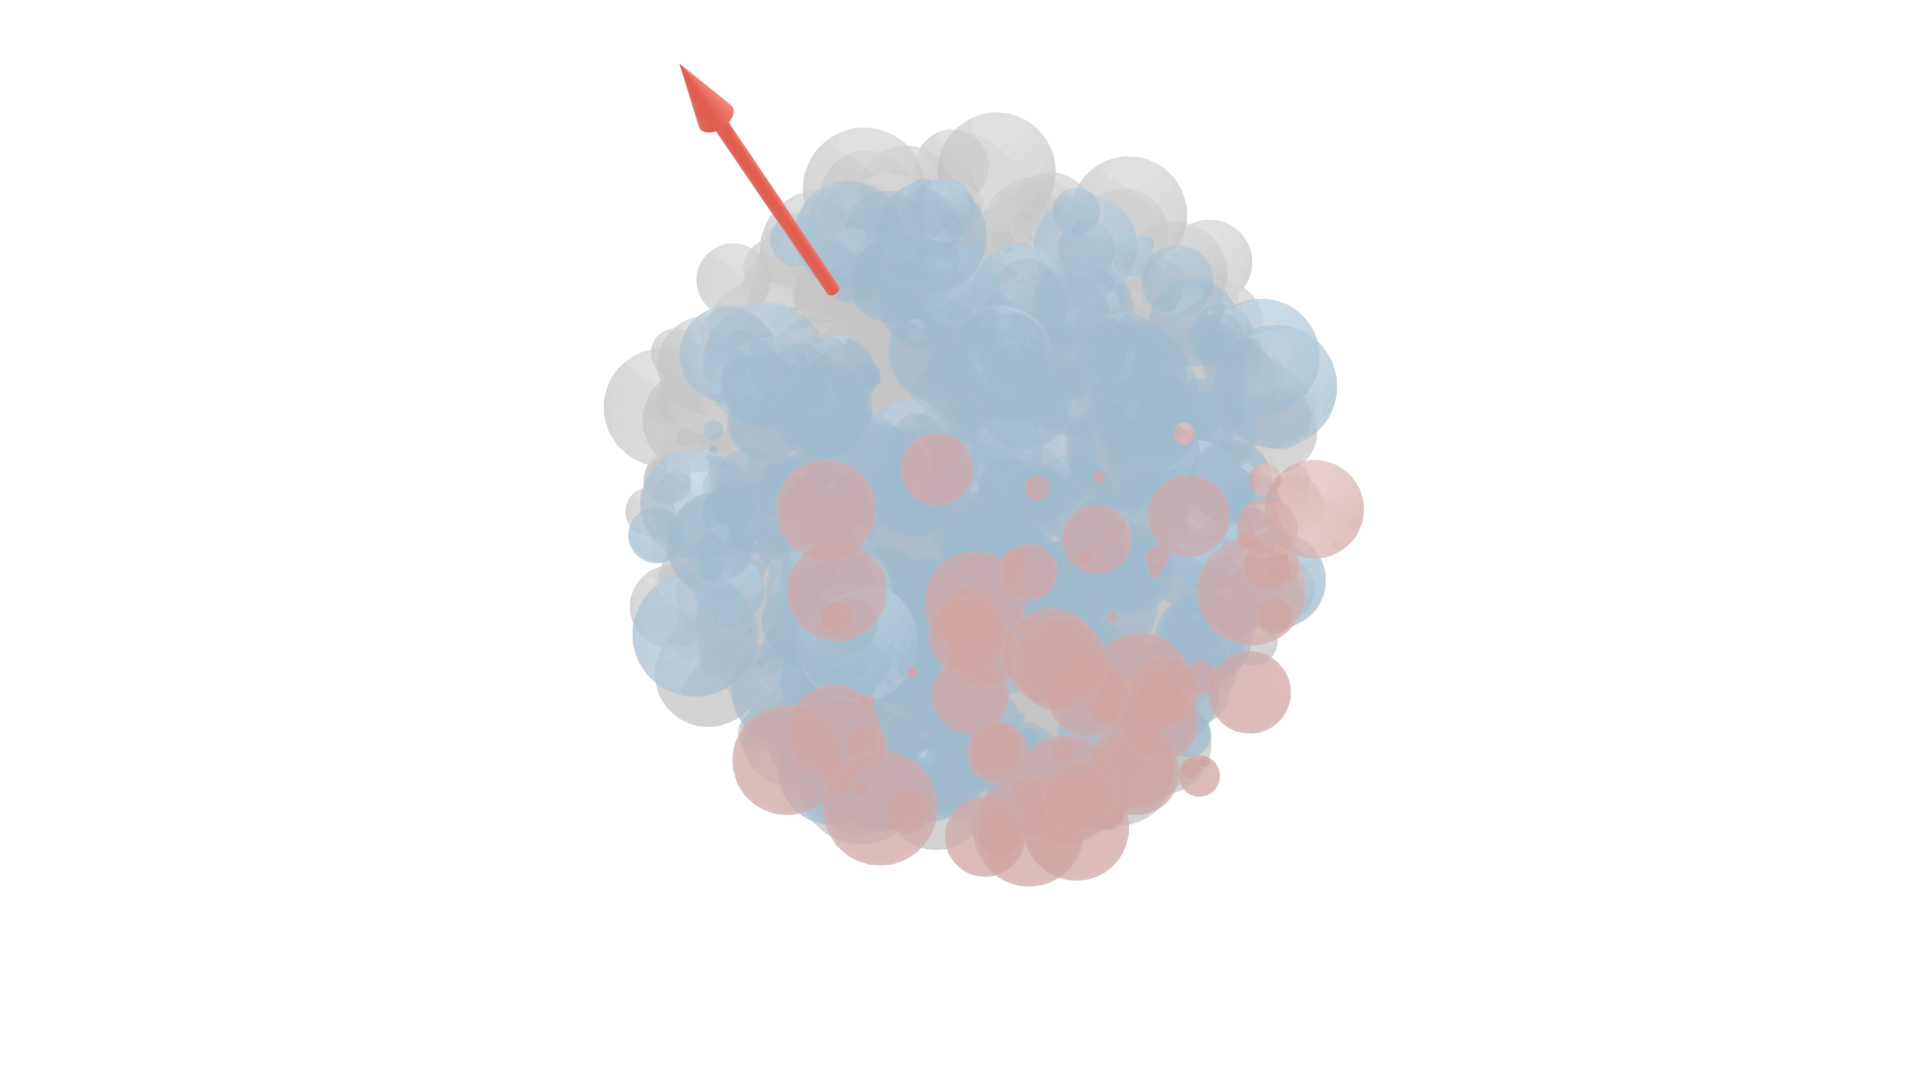
\includegraphics[width=\linewidth]{fig3}
\end{center}
\caption{The free electron (artistic impression, not a rendered simulation). \label{fig:electron} Conjectured composition of a free electron as an aggregate of charge fragments.  The red bubbles are drive pairs; the red arrow marks the resultant direction of their momentum vectors (the electron's net propagation direction, not a magnetic field line).  The blue bubbles are negative-charge singletons, and the gray bubbles are electron--neutrino pairs.  Length scale is arbitrary; the figure is a schematic of the six-bit charge algebra, not an output of the automaton.}
\end{figure}
\paragraph{The muon neutrino.}
The muon neutrino $\nu_{\mu}$ is conjectured to be formed as $\nu_{\mu}=2\nu_e+\bar{\nu}_e$ plus additional drive pairs.
It would be like an electron neutrino, but with a compensated antimatter part.
\paragraph{The muon.}
The muon $\mu^-$ is conjectured to consist of a quantized number of $-L$ fragments, a large number of muon neutrinos $\nu_{\mu}$, and a variable number of drive pairs.
The classical study conducted by It\^{o} in \cite{ito} suggests that this configuration stabilizes at the second harmonic of the electron's radial vibrational state.
\paragraph{The tau neutrino.}
The tau neutrino $\nu_{\tau}$ is conjectured to be formed as $\nu_{\tau}=3\nu_e+2\bar{\nu}_e$ plus additional drive pairs.
It would also be like an electron neutrino, but with a compensated antimatter-enriched part.
\paragraph{The tau.}
The tau $\tau^-$ is conjectured to be formed by a quantized number of $-L$ fragments, a great number of tau neutrinos $\nu_{\mu}$, and a variable number of drive pairs.
\paragraph{Gauge bosons.}
These bosons were described in Sect. \ref{bosons}.
\paragraph{Leptons decay.}
In the Standard Model (SM), the decay products typically include one neutrino or antineutrino.
In our model, one might conjecture that the large number of neutrinos in a particle is entangled by a common affinity, so that when one neutrino interacts via the weak force, all other entangled neutrinos collapse to the same point.
Under that conjecture, the observable outcome would be indistinguishable from a single, energetic neutrino, in agreement with the SM prediction.
If the neutrino belongs to the other sector (Orbis/Umbra), spontaneous decay might follow.  None of this behavior has been observed in the implementation.
\paragraph{Electronic decay.}
After the absorption of (part of) a photon, the electron would, under the model, enter an excited state, dynamically stabilizing in a suitable spherical harmonic configuration.
When the common components of the photon and electron are reissued, the odds of a configuration corresponding to the original photon are less than one.
As time passes, after many cohesion interactions, the proper configuration of charges and pBits may occur, forming a single photonic cluster and allowing the emitted photon to escape the frequent reissue mechanism, fleeing away from the electron cloud, which eventually settles into its ground state.
\paragraph{Compound particles half-lives.}
Protons, electrons, and electron neutrinos are, under the model, composed exclusively of bubbles, without their corresponding anti-bubbles.
This unique composition is offered as a key factor in their exceptionally long half-lives, potentially making them stable.
In contrast, particles containing both bubbles and anti-bubbles are conjectured to be significantly less stable.
Their shorter half-lives would result from the likelihood of annihilation events between bubbles and anti-bubbles within their structure, leading to their transient nature.
The neutron would, under the model, embed lots of electron antineutrinos, which bind the negative charge to its inner proton.
This is offered as a possible explanation of the free neutron decay.
\[
n^0\rightarrow\,p^{+}+e^{-}+\nu_e
\]
\paragraph{Nuclear decay.}
In this model, nuclear decay processes emerge from the internal structure and composition of compound particles representing atomic nuclei.
These instabilities trigger reorganizations via the electroweak collapse mechanism, where the sieve test result ($s2B$) determines the feasibility of transformations.
The decay process is similar to the free neutron decay seen above.
The perturbing particles are typically neutrinos and Z bosons that permeate the vacuum. Once again, if these perturbing particles belong to the other sector (Orbis/Umbra), then we have spontaneous decay.
This internal annihilation mechanism is offered as a possible account of decay processes; whether it reproduces the empirical tables of nuclides is not established, since no nuclear-scale configuration has been simulated.
\paragraph{Heavier quarks.}
The framework speculatively suggests that the other quarks could follow the composition of leptons, with additional neutrinos and antineutrinos, besides a variable number of drive pairs.
\paragraph{Atoms.}
Bound states of protons, neutrons, and electrons might naturally be expected in this scenario; their formation is not demonstrated by the current implementation.
\paragraph{The abundance of neutrinos.}
Despite the relatively small number of neutrinos observed in Table \ref{tab:color-combination}, their large cosmic abundance reflects their low mass, approximately five million times smaller than the mass of an electron.
This characteristic allows neutrinos to exist in enormous quantities across the universe, even if their presence appears limited.
\end{document}
